% Digital Floats Controller - User Manual
% Based on ATA iSpec 2200
% Created for Skymatik Aero

% Document class
\documentclass[12pt,a4paper,twoside,openright]{book}

% Required packages
\usepackage{geometry}
\usepackage{fontspec}
\usepackage{titlesec}
\usepackage{titletoc}
\usepackage{fancyhdr}
\usepackage{graphicx}
\usepackage{xcolor}
\usepackage{tocloft}
\usepackage{hyperref}
\usepackage{setspace}
\usepackage{lipsum}  % For placeholder text
\usepackage{tikz}    % For logo generation
\usepackage{tabularx}
\usepackage{booktabs}
\usepackage{array}

% Document geometry
\geometry{a4paper, margin=1in, bottom=1.25in}

% Font settings
\setmainfont{Arial}

% Line spacing
\setstretch{1.4}

% Color definitions
\definecolor{skyblue}{RGB}{41, 128, 185}
\definecolor{navyblue}{RGB}{24, 59, 86}
\definecolor{titlewhite}{RGB}{255, 255, 255}
\definecolor{missingred}{RGB}{220, 50, 50}

% Chapter numbering
\renewcommand{\thechapter}{\arabic{chapter}}

% Chapter formatting - left-aligned titles
\titleformat{\chapter}[display]
  {\normalfont\huge\bfseries\color{skyblue}\raggedright}
  {\huge\bfseries Chapter \thechapter}
  {20pt}
  {\raggedright\Huge\bfseries}
  [\vspace{1ex}{\color{skyblue}\titlerule[2pt]}]

\titlespacing*{\chapter}{0pt}{80pt}{40pt}

% Make chapters start on right-hand pages (odd pages)
\makeatletter
\renewcommand\chapter{\if@openright\cleardoublepage\else\clearpage\fi
                    \thispagestyle{plain}%
                    \global\@topnum\z@
                    \@afterindentfalse
                    \secdef\@chapter\@schapter}
\makeatother

% Blank page style for empty pages
\makeatletter
\def\cleardoublepage{\clearpage\if@twoside \ifodd\c@page\else
    \vspace*{\fill}
    \begin{center}
    \textit{This page intentionally left blank}
    \end{center}
    \vspace{\fill}
    \thispagestyle{empty}
    \newpage
    \if@twocolumn\hbox{}\newpage\fi\fi\fi}
\makeatother

% Section formatting
\titleformat{\section}
{\normalfont\Large\bfseries\color{navyblue}}
{}{0em}{\thesection\ }
\titlespacing*{\section}{0pt}{3.5ex plus 1ex minus .2ex}{2.3ex plus .2ex}

% Subsection formatting
\titleformat{\subsection}
{\normalfont\large\bfseries\color{navyblue}}
{}{0em}{\thesubsection\ }
\titlespacing*{\subsection}{0pt}{3.25ex plus 1ex minus .2ex}{1.5ex plus .2ex}

% Header and footer - increase spacing to prevent overlap
\pagestyle{fancy}
\fancyhf{}

% Modified chapter marking commands
\renewcommand{\chaptermark}[1]{\markboth{#1}{#1}}
\renewcommand{\sectionmark}[1]{\markright{#1}}

% Left and right headers with exactly two lines and proper alignment
\fancyhead[RO]{\begin{tabular}[t]{r}\textit{Digital Floats Controller}\\\textit{User Manual}\end{tabular}}
\fancyhead[LE]{\begin{tabular}[t]{l}\textit{Digital Floats Controller}\\\textit{User Manual}\end{tabular}}
\fancyhead[LO]{\begin{tabular}[t]{l}\textit{Chapter \thechapter}\\\textit{\nouppercase{\leftmark}}\end{tabular}}
\fancyhead[RE]{\begin{tabular}[t]{r}\textit{Chapter \thechapter}\\\textit{\nouppercase{\leftmark}}\end{tabular}}

% Page numbers in footer with correct alignment
\fancyfoot[RO]{\thepage}
\fancyfoot[LE]{\thepage}

% Header/footer rules
\renewcommand{\headrulewidth}{0.4pt}
\renewcommand{\footrulewidth}{0.4pt}

% Increase header height to accommodate two lines
\setlength{\headheight}{30pt}

% Hyperlink settings
\hypersetup{
    colorlinks=true,
    linkcolor=skyblue,
    filecolor=skyblue,
    urlcolor=skyblue,
    citecolor=skyblue,
    pdftitle={Digital Floats Controller -- User Manual},
    pdfauthor={Skymatik Aero},
}

% For front matter (roman numerals)
\frontmatter

% Set the graphicspath to include the images directory
\graphicspath{{images/}}

% Table of contents formatting
\renewcommand{\cftaftertoctitle}{\vspace{2em}}
\renewcommand{\cftbeforetoctitleskip}{0pt}
\renewcommand{\cftaftertoctitleskip}{1em}
\setlength{\cftbeforechapskip}{0.5em}
\setlength{\cftbeforesecskip}{0.25em}

% Style the TOC title to match the document style
\renewcommand{\cfttoctitlefont}{\Huge\bfseries\color{skyblue}}
\renewcommand{\contentsname}{Table of Contents}

% Add dotted leaders for chapters
\renewcommand{\cftchapdotsep}{\cftdotsep}

% Indent section numbers properly
\setlength{\cftsecindent}{2em}
\setlength{\cftsubsecindent}{4em}

% Footer settings - ensure footer has enough space
\setlength{\footskip}{40pt}  % Increase space for footer

% Define plain page style for chapter pages
\fancypagestyle{plain}{%
  \fancyhf{} % Clear all headers and footers
  \renewcommand{\headrulewidth}{0pt} % No header rule
  \renewcommand{\footrulewidth}{0pt} % No footer rule
  \fancyfoot[RO,LE]{\thepage} % Page number in the footer
}

% Table spacing and style commands
\newcommand{\tabletextfont}{\normalfont\rmfamily}
\newcommand{\tableheadfont}{\normalfont\bfseries}
\renewcommand{\arraystretch}{1.3} % Increase vertical spacing in tables

\begin{document}

% Title page using PNG image as full cover
\begin{titlepage}
    \thispagestyle{empty}
    % Save the current page dimensions
    \newlength{\currentparindent}
    \setlength{\currentparindent}{\parindent}
    % Remove all page margins
    \newgeometry{left=0mm, right=0mm, top=0mm, bottom=0mm}
    % Remove paragraph indentation
    \setlength{\parindent}{0mm}
    % Place the image
    \noindent\makebox[\linewidth]{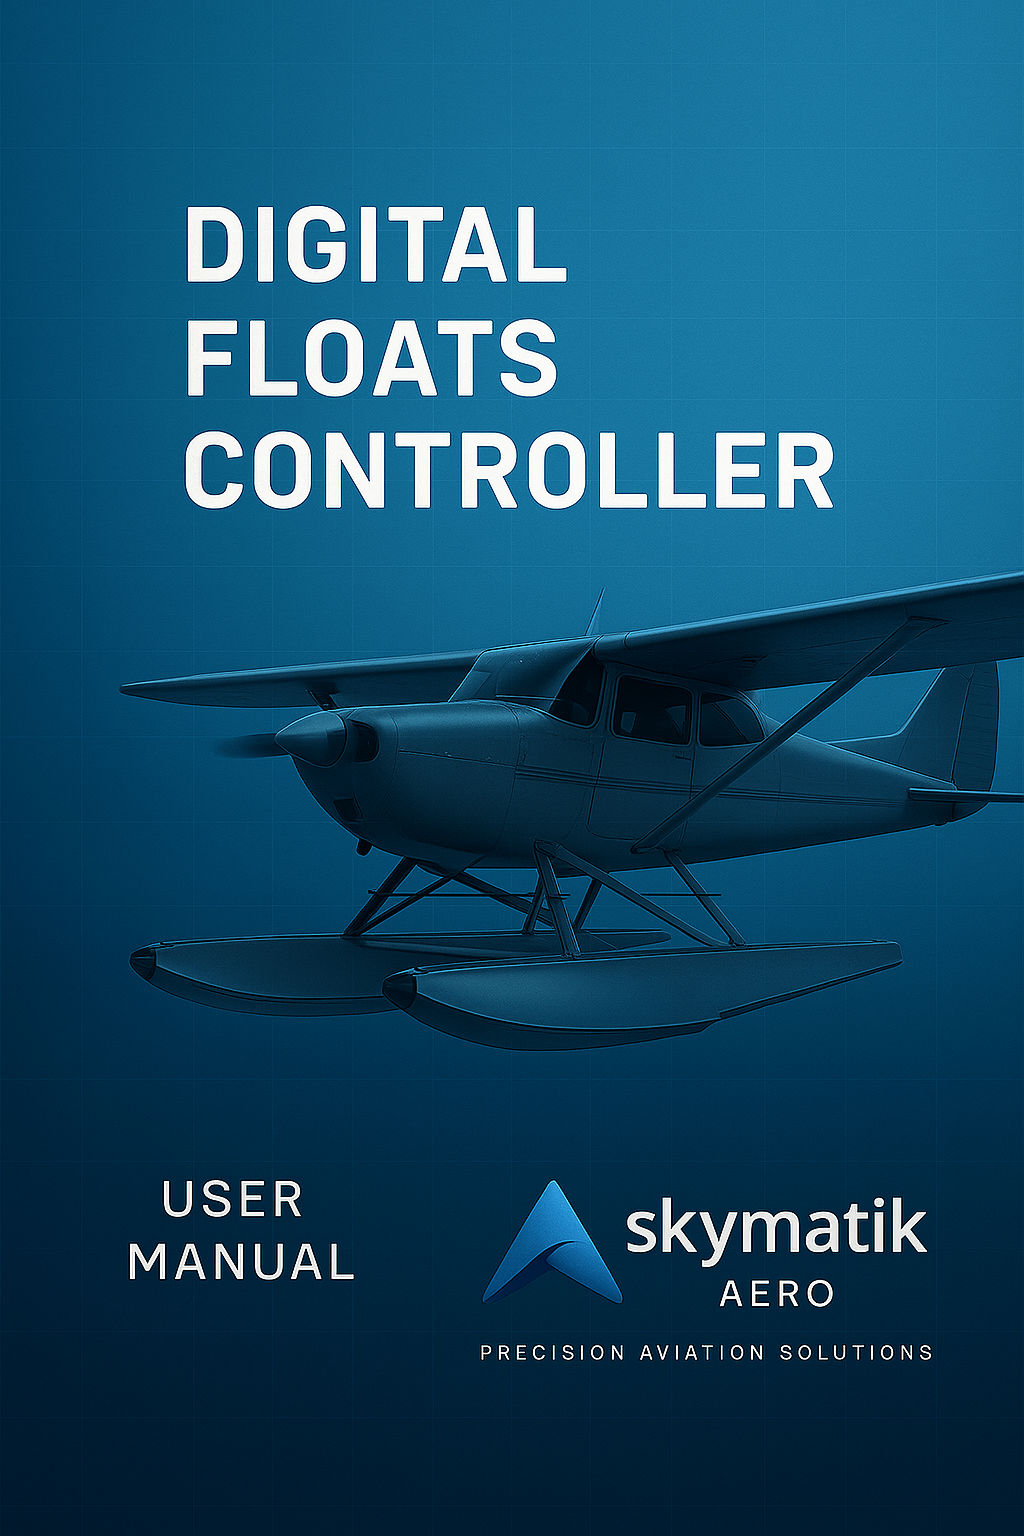
\includegraphics[width=\paperwidth,height=\paperheight]{front_page_manual.png}}
    % Restore the geometry for subsequent pages
    \clearpage
    \restoregeometry
    \setlength{\parindent}{\currentparindent}
\end{titlepage}

% Thank You Letter
\cleardoublepage
\thispagestyle{fancy}
\vspace*{2cm}
\begin{center}
{\Large\bfseries\color{skyblue}THANK YOU}
\end{center}

\vspace{1cm}

\begin{quote}
Dear Valued Customer,

On behalf of everyone at Skymatik Aero, we would like to express our sincere gratitude for choosing the Digital Floats Control System for your aircraft. Your trust in our products is the foundation of our success and drives our commitment to excellence.

The system you have purchased represents years of research, development, and rigorous testing to ensure it meets the highest standards of quality, reliability, and safety in the aviation industry. We are confident that it will enhance your aircraft's capabilities and provide you with many years of trouble-free operation.

This comprehensive manual has been carefully prepared to help you install, operate, and maintain your Digital Floats Control System. We encourage you to read it thoroughly before installation and operation, and to keep it as a reference for future maintenance needs.

Thank you once again for your business and for being part of the Skymatik Aero family.

\vspace{0.5cm}

Sincerely,

\vspace{1cm}

\begin{flushright}
\begin{tabular}{c}
\rule{5cm}{0.4pt} \\
The Skymatik Aero Team
\end{tabular}
\end{flushright}
\end{quote}

\clearpage

% Table of contents
\cleardoublepage
\phantomsection
\addcontentsline{toc}{chapter}{\contentsname}
\tableofcontents
\thispagestyle{fancy}  % Apply the fancy style to ensure header and footer appear
\clearpage

% Main matter (arabic numerals)
\mainmatter

% Adding custom chapter for Preface that starts at 0
\setcounter{chapter}{-1}
\chapter{Preface}
\setcounter{page}{1}

\section{Document Control}

\begin{table}[h]
\centering
\setlength{\tabcolsep}{5pt} % Reduce column spacing
\begin{tabular}{|p{0.4\textwidth}|p{0.5\textwidth}|}
\hline
\tableheadfont\textbf{Parameter} & \tableheadfont\textbf{Value} \\
\hline
\tabletextfont Document Identifier & DFC-UM-001 \\
\hline
\tabletextfont Issue/Revision Number & 1.0 \\
\hline
\tabletextfont Publication Date & {\color{missingred}[Required: Publication date in DD-MMM-YYYY format]} \\
\hline
\end{tabular}
\caption{Document Identification}
\end{table}

\subsection{Revision History}

\begin{table}[h]
\centering
\setlength{\tabcolsep}{4pt} % Reduce column spacing
\begin{tabular}{|p{0.15\textwidth}|p{0.1\textwidth}|p{0.4\textwidth}|p{0.25\textwidth}|}
\hline
\tableheadfont\textbf{Date} & \tableheadfont\textbf{Version} & \tableheadfont\textbf{Changes} & \tableheadfont\textbf{Approved By} \\
\hline
\tabletextfont {\color{missingred}[Date]} & 0.1 & Initial draft & {\color{missingred}[Name]} \\
\hline
\tabletextfont {\color{missingred}[Date]} & 0.5 & Technical content review & {\color{missingred}[Name]} \\
\hline
\tabletextfont {\color{missingred}[Date]} & 0.9 & Pre-release candidate & {\color{missingred}[Name]} \\
\hline
\tabletextfont {\color{missingred}[Date]} & 1.0 & First production release & {\color{missingred}[Name]} \\
\hline
\end{tabular}
\caption{Revision History}
\end{table}

\subsection{Distribution List}

\begin{table}[h]
\centering
\setlength{\tabcolsep}{5pt} % Reduce column spacing
\begin{tabular}{|p{0.3\textwidth}|p{0.2\textwidth}|p{0.4\textwidth}|}
\hline
\tableheadfont\textbf{Organization} & \tableheadfont\textbf{Copy Type} & \tableheadfont\textbf{Number of Copies} \\
\hline
\tabletextfont Skymatik Aero Engineering & Controlled & Master copy \\
\hline
\tabletextfont Skymatik Aero QA Department & Controlled & 1 \\
\hline
\tabletextfont Production Department & Controlled & 1 \\
\hline
\tabletextfont Customer Support & Controlled & 1 \\
\hline
\tabletextfont Installation/Maintenance Facilities & Controlled & As required \\
\hline
\tabletextfont Aircraft Operators & Controlled & Provided with each system \\
\hline
\end{tabular}
\caption{Distribution List}
\end{table}

\section{Authorship and Approval}

\begin{table}[h]
\centering
\setlength{\tabcolsep}{5pt} % Reduce column spacing
\begin{tabular}{|p{0.3\textwidth}|p{0.6\textwidth}|}
\hline
\tableheadfont\textbf{Role} & \tableheadfont\textbf{Name and Position} \\
\hline
\tabletextfont Principal Author & {\color{missingred}[Name, Position]} \\
\hline
\tabletextfont Contributing Authors & {\color{missingred}[Names, Positions]} \\
\hline
\tabletextfont Technical Reviewers & {\color{missingred}[Names, Positions]} \\
\hline
\tabletextfont Quality Assurance & {\color{missingred}[Name, Position]} \\
\hline
\tabletextfont Final Approval Authority & {\color{missingred}[Name, Position]} \\
\hline
\end{tabular}
\caption{Document Authorship}
\end{table}

\vspace{1cm}
\subsection{Signatures of Approval}

\begin{table}[h]
\centering
\setlength{\tabcolsep}{5pt} % Reduce column spacing
\begin{tabular}{|p{0.3\textwidth}|p{0.3\textwidth}|p{0.25\textwidth}|}
\hline
\tableheadfont\textbf{Role} & \tableheadfont\textbf{Signature} & \tableheadfont\textbf{Date} \\
\hline
\tabletextfont Engineering Manager & & \\
\hline
\tabletextfont Quality Assurance Manager & & \\
\hline
\tabletextfont Technical Publications Manager & & \\
\hline
\tabletextfont Chief Engineer & & \\
\hline
\end{tabular}
\caption{Approval Signatures}
\end{table}

\section{Copyright and Proprietary Information}

\subsection{Copyright Statement}

\begin{quote}
© {\color{missingred}[Year]} Skymatik Aero. All rights reserved. No part of this publication may be reproduced, stored in a retrieval system, or transmitted in any form or by any means, electronic, mechanical, photocopying, recording, or otherwise, without the prior written permission of Skymatik Aero.
\end{quote}

\subsection{Proprietary Notices}

\begin{quote}
This document contains proprietary and confidential information of Skymatik Aero. The information contained herein may not be disclosed or distributed to any third party without the express written consent of Skymatik Aero.
\end{quote}

\subsection{Export Control Classification}

\begin{quote}
This document contains technical data whose export may be restricted by the Export Administration Regulations (EAR) or the International Traffic in Arms Regulations (ITAR). Violations of these export laws are subject to severe criminal penalties.

Export Control Classification Number (ECCN): {\color{missingred}[Classification number]}

ITAR Category: {\color{missingred}[ITAR category, if applicable]}
\end{quote}

\subsection{Confidentiality Level}

\begin{quote}
Confidentiality classification: For official use only. Authorized distribution to certified aircraft operators, maintenance personnel, and regulatory authorities only.
\end{quote}

\section{How to Use This Document}

\subsection{Document Organization}

This user manual is organized into chapters that follow the logical sequence of understanding, installing, operating, and maintaining the Digital Floats Control System:

\begin{itemize}
    \item \textbf{Chapter 1: General Information} - Provides an overview of the system, its purpose, and basic technical specifications.
    \item \textbf{Chapter 2: Construction and Technical Characteristics} - Details the technical design, components, and specifications of the system.
    \item \textbf{Chapter 3: Equipment Installation} - Contains procedures and requirements for installing the system in an aircraft.
    \item \textbf{Chapter 4: Operation} - Explains how to operate the system during normal and emergency conditions.
    \item \textbf{Chapter 5: Integration with Other Systems} - Describes how the system interfaces with other aircraft systems.
    \item \textbf{Chapter 6: Technical Maintenance and Servicing} - Outlines maintenance schedules and procedures.
    \item \textbf{Chapter 7: Troubleshooting and Diagnostics} - Provides guidance for identifying and resolving common issues.
    \item \textbf{Chapter 8: Certification and Compliance} - Documents regulatory compliance information.
    \item \textbf{Chapter 9: Spare Parts and Logistics} - Lists spare parts and ordering information.
    \item \textbf{Chapter 10: Modifications and Updates} - Explains the process for system updates and modifications.
    \item \textbf{Chapter 11: Training} - Outlines training requirements for operators and maintenance personnel.
    \item \textbf{Chapter 12: Appendices} - Contains supplementary information and reference materials.
\end{itemize}

\subsection{Navigation Aids}

This manual includes several navigation aids to help you quickly find specific information:

\begin{itemize}
    \item \textbf{Table of Contents} - Lists all chapters, sections, and subsections with page numbers.
    \item \textbf{Headers and Footers} - Each page header shows the chapter title and manual title for easy orientation.
    \item \textbf{Cross-References} - References to related information are provided as hyperlinks in the electronic version.
    \item \textbf{Tables and Figures} - All tables and figures are numbered sequentially within each chapter.
    \item \textbf{Index} - A comprehensive index is provided at the end of the manual.
\end{itemize}

\subsection{Conventions Used}

The following conventions are used throughout this manual:

\begin{itemize}
    \item \textbf{Bold Text} - Used for emphasis, UI elements, and physical controls.
    \item \textit{Italic Text} - Used for document titles, references, and parameter values.
    \item \texttt{Monospace Text} - Used for configuration parameters and values.
    \item \colorbox{yellow}{\textbf{WARNING}} - Indicates a potentially hazardous situation which, if not avoided, could result in death or serious injury.
    \item \colorbox{orange}{\textbf{CAUTION}} - Indicates a potentially hazardous situation which, if not avoided, may result in minor or moderate injury, or damage to equipment.
    \item \colorbox{lightgray}{\textbf{NOTE}} - Provides additional information, tips, or reminders.
    \item {\color{missingred}[Required Information]} - Indicates information that must be filled in based on the specific installation.
\end{itemize}

\subsection{Related Documentation}

The following documents provide additional information related to the Digital Floats Control System:

\begin{itemize}
    \item DFC-ICA-001: Instructions for Continued Airworthiness
    \item DFC-IM-001: Installation Manual
    \item DFC-CD-001: Component Design Document
    \item DFC-QTP-001: Qualification Test Procedures
    \item DFC-SW-001: Software Description Document
    \item {\color{missingred}[Additional related documents specific to aircraft type or installation]}
\end{itemize}

\section{Revision Policy}

\subsection{Process for Requesting Changes}

To request changes to this document:

\begin{enumerate}
    \item Submit change requests in writing to the address provided in the Contact Information section.
    \item Include the document identifier, revision number, specific section/page requiring change, proposed change text, and justification.
    \item For operators and maintenance facilities, submit changes through your technical representative or the online support portal.
    \item Internal staff should use the document control system to submit change requests.
\end{enumerate}

All proposed changes will be reviewed by the technical team and implemented according to the established configuration management procedures.

\subsection{Update Frequency}

This document is updated according to the following schedule:

\begin{itemize}
    \item Major revisions: Annually or with significant system changes
    \item Minor revisions: Quarterly or as needed
    \item Immediate updates: For safety-critical information
\end{itemize}

\subsection{Distribution of Updates}

Updates to this document are distributed through the following channels:

\begin{itemize}
    \item Electronic notifications to all registered users
    \item Publication on the secure Skymatik Aero technical portal
    \item Physical distribution of updated pages or complete manuals for controlled copies
    \item Service Bulletins for critical updates
\end{itemize}

\subsection{Configuration Management}

This document is controlled according to the Skymatik Aero Configuration Management Plan (CMP-001). Key procedures include:

\begin{itemize}
    \item All changes are tracked in the document control system
    \item Each revision undergoes technical and editorial review
    \item Final approval required before release
    \item Obsolete versions are archived according to regulatory requirements
    \item Change history is maintained for the life of the product
\end{itemize}

\section{Contact Information}

\subsection{Technical Support}

For technical support related to the Digital Floats Control System:

\begin{itemize}
    \item Phone: {\color{missingred}[Support phone number]}
    \item Email: {\color{missingred}[Support email address]}
    \item Online: {\color{missingred}[Support website URL]}
    \item Hours of Operation: {\color{missingred}[Hours and time zone]}
\end{itemize}

\subsection{Feedback Submission}

To submit feedback on this document or the Digital Floats Control System:

\begin{itemize}
    \item Email: {\color{missingred}[Feedback email address]}
    \item Online Form: {\color{missingred}[Feedback form URL]}
    \item Postal Mail:
    
    {\color{missingred}[Company name]}
    
    {\color{missingred}[Street address]}
    
    {\color{missingred}[City, State/Province, Postal Code]}
    
    {\color{missingred}[Country]}
\end{itemize}

\subsection{Emergency Contacts}

For urgent issues requiring immediate assistance:

\begin{itemize}
    \item 24/7 Emergency Support: {\color{missingred}[Emergency phone number]}
    \item AOG (Aircraft on Ground) Support: {\color{missingred}[AOG support contact]}
\end{itemize}

\section{List of Effective Pages}

\begin{table}[h]
\centering
\setlength{\tabcolsep}{4pt} % Reduce column spacing
\begin{tabular}{|p{0.15\textwidth}|p{0.15\textwidth}|p{0.15\textwidth}|p{0.15\textwidth}|p{0.15\textwidth}|}
\hline
\tableheadfont\textbf{Section} & \tableheadfont\textbf{Page} & \tableheadfont\textbf{Revision} & \tableheadfont\textbf{Date} & \tableheadfont\textbf{Status} \\
\hline
\tabletextfont Front Matter & i-viii & 1.0 & {\color{missingred}[Date]} & Current \\
\hline
\tabletextfont Chapter 0 & 0-1 to 0-10 & 1.0 & {\color{missingred}[Date]} & Current \\
\hline
\tabletextfont Chapter 1 & 1-1 to 1-10 & 1.0 & {\color{missingred}[Date]} & Current \\
\hline
\tabletextfont Chapter 2 & 2-1 to 2-12 & 1.0 & {\color{missingred}[Date]} & Current \\
\hline
\tabletextfont Chapter 3 & 3-1 to 3-15 & 1.0 & {\color{missingred}[Date]} & Current \\
\hline
\tabletextfont Chapter 4 & 4-1 to 4-18 & 1.0 & {\color{missingred}[Date]} & Current \\
\hline
\tabletextfont Chapter 5 & 5-1 to 5-8 & 1.0 & {\color{missingred}[Date]} & Current \\
\hline
\tabletextfont Chapter 6 & 6-1 to 6-10 & 1.0 & {\color{missingred}[Date]} & Current \\
\hline
\tabletextfont Chapter 7 & 7-1 to 7-12 & 1.0 & {\color{missingred}[Date]} & Current \\
\hline
\tabletextfont Chapter 8 & 8-1 to 8-6 & 1.0 & {\color{missingred}[Date]} & Current \\
\hline
\tabletextfont Chapter 9 & 9-1 to 9-8 & 1.0 & {\color{missingred}[Date]} & Current \\
\hline
\tabletextfont Chapter 10 & 10-1 to 10-6 & 1.0 & {\color{missingred}[Date]} & Current \\
\hline
\tabletextfont Chapter 11 & 11-1 to 11-4 & 1.0 & {\color{missingred}[Date]} & Current \\
\hline
\tabletextfont Chapter 12 & 12-1 to 12-10 & 1.0 & {\color{missingred}[Date]} & Current \\
\hline
\end{tabular}
\caption{List of Effective Pages}
\end{table}

\section{Document Scope}

\subsection{Coverage}

This manual covers:

\begin{itemize}
    \item Complete technical description of the Digital Floats Control System
    \item Detailed installation procedures
    \item Operational instructions for normal and emergency situations
    \item Maintenance procedures and schedules
    \item Troubleshooting guidelines
    \item Configuration, calibration, and adjustment procedures
    \item Regulatory compliance information
    \item Parts information and ordering procedures
\end{itemize}

\subsection{Exclusions}

This manual does not cover:

\begin{itemize}
    \item Advanced repair procedures requiring factory support
    \item Details of aircraft-specific modifications beyond standard installations
    \item Development and verification test procedures
    \item Internal software architecture and code-level details
    \item Manufacturing processes and quality control procedures
    \item Detailed circuit diagrams and component-level repair
\end{itemize}

\subsection{Target Audience}

This document is intended for:

\begin{itemize}
    \item Aircraft installation technicians and mechanics
    \item Aircraft operators and pilots
    \item Maintenance personnel
    \item Aviation regulatory authorities
    \item Aircraft modification centers
    \item Technical support personnel
\end{itemize}

The manual assumes the reader has:

\begin{itemize}
    \item Basic understanding of aircraft systems
    \item Familiarity with avionics equipment
    \item Proper certification or authorization for installation and maintenance
    \item Access to standard aviation tools and test equipment
    \item Knowledge of aviation regulations and standards
\end{itemize}

% Reset chapter counter to properly start at Chapter 1
\setcounter{chapter}{0}
\chapter{General Information}
\newpage % Start content on a new page

\section{Purpose of the Equipment}
The Digital Floats Control System is designed to manage and control the gear mechanisms in aircraft equipped with floats, enabling safe transitions between land and water operations. The system provides pilots with reliable control over landing gear and rudder positions, crucial for amphibious aircraft that need to operate on both land and water surfaces.

This control system manages up to four landing gear actuators and one rudder actuator, continuously monitoring their positions through limit switches and providing real-time status via LED indicators. The system implements comprehensive error detection and safety features to prevent improper gear configuration during critical flight phases.

\section{General Description and Operating Principles}

\subsection{System Overview}
The Digital Floats Control System features a user interface with two physical switches and five RGB LED indicators. The left switch controls the landing gear, while the right switch controls the rudder. Four LEDs display the status of the four landing gear positions, and the fifth LED shows the status of the rudder.

\subsection{Operating Modes}
The system operates in three distinct modes, each with specific gear and rudder configurations:

\begin{table}[h]
\centering
\setlength{\tabcolsep}{4pt} % Reduce column spacing
\begin{tabular}{|p{0.18\textwidth}|p{0.22\textwidth}|p{0.22\textwidth}|p{0.26\textwidth}|}
\hline
\tableheadfont\textbf{Mode} & \tableheadfont\textbf{Gear Position} & \tableheadfont\textbf{Rudder Position} & \tableheadfont\textbf{Switch Positions} \\
\hline
\tabletextfont Land Mode & Extended & Retracted & Gear switch down, rudder switch up/down \\
\hline
\tabletextfont Water Mode & Retracted & Retracted & Gear switch up, rudder switch up \\
\hline
\tabletextfont Maneuver Mode & Retracted & Extended & Gear switch up, rudder switch down \\
\hline
\end{tabular}
\caption{Operating Modes of the Digital Floats Control System}
\end{table}

\subsection{Basic Operation}
When pilots toggle the gear or rudder switches, the system activates the appropriate actuators to move the gear or rudder to the requested position. The system monitors the movement through limit switches and automatically stops the actuators when the end positions are reached. RGB LED indicators provide continuous visual feedback about current positions and any detected issues.

\subsection{Self-Test Procedure}
Upon powering up, the system automatically performs a comprehensive self-test sequence to verify:
\begin{itemize}
    \item I2C device connectivity (sensors and I/O expanders)
    \item RTC (Real-Time Clock) functionality
    \item External memory integrity
    \item Actuator circuit continuity
    \item Limit switch functionality
\end{itemize}

Results of the self-test are displayed via the RGB LEDs, providing immediate feedback about system health.

\section{Basic Technical Data and Parameters}

\begin{table}[h]
\centering
\setlength{\tabcolsep}{5pt} % Reduce column spacing
\begin{tabular}{|p{0.35\textwidth}|p{0.55\textwidth}|}
\hline
\tableheadfont\textbf{Parameter} & \tableheadfont\textbf{Specification} \\
\hline
\tabletextfont Microcontroller & STM32F103 (ARM Cortex-M3) \\
\hline
\tabletextfont Operating Voltage & 8V to 28V DC \\
\hline
\tabletextfont Maximum Current per Channel & 5A \\
\hline
\tabletextfont Number of Control Channels & 5 (4 landing gear + 1 rudder) \\
\hline
\tabletextfont Communication Interface & UART \\
\hline
\tabletextfont Status Indicators & 5 RGB LEDs (WS2812) \\
\hline
\tabletextfont User Controls & 2 Toggle Switches \\
\hline
\tabletextfont Limit Switch Support & Normally Open (NO) or Normally Closed (NC) \\
\hline
\tabletextfont Current Sensing Range & 0.1A to 5.0A \\
\hline
\tabletextfont Voltage Sensing Range & 8.0V to 28.0V \\
\hline
\tabletextfont Temperature Range & {\color{missingred}[Required: Operating temperature range in °C, including storage and operational limits per DO-160 standards]} \\
\hline
\tabletextfont Dimensions & {\color{missingred}[Required: Physical dimensions of control unit in mm (L × W × H)]} \\
\hline
\tabletextfont Weight & {\color{missingred}[Required: Weight of control unit in grams]} \\
\hline
\end{tabular}
\caption{Technical Specifications of the Digital Floats Control System}
\end{table}

\section{Operational Limitations}

The Digital Floats Control System has the following operational limitations:

\begin{itemize}
    \item \textbf{Voltage Limitations:} The system requires a power supply between 8.0V and 28.0V DC. Operation outside this range may cause erratic behavior or damage to the system.
    
    \item \textbf{Current Limitations:} Each actuator channel is limited to a maximum of 5.0A. Actuators drawing more current will trigger an overcurrent protection.
    
    \item \textbf{Temperature Range:} {\color{missingred}[Required: Operational temperature range specification per DO-160G Section 4 compliance, including both normal and short-term extremes]}
    
    \item \textbf{Actuator Compatibility:} The system is designed to work with electric actuators equipped with limit switches. Hydraulic or pneumatic systems require additional interface hardware.
    
    \item \textbf{Simultaneous Channel Operation:} The system can operate multiple channels simultaneously, but users should be aware of potential current draw limitations when all channels are active.
\end{itemize}

\section{Compliance with Regulations and Standards}

The Digital Floats Control System is designed to comply with the following aviation regulations and standards:

\begin{itemize}
    \item \textbf{DO-160:} Environmental Conditions and Test Procedures for Airborne Equipment
    \item \textbf{DO-254:} Design Assurance Guidance for Airborne Electronic Hardware
    \item \textbf{DO-178C:} Software Considerations in Airborne Systems and Equipment Certification
    \item \textbf{FAR Part 23:} Airworthiness Standards for Normal Category Aircraft
    \item \textbf{ASTM F3153:} Standard Specification for Verification of Avionics Systems
\end{itemize}

{\color{missingred}[Required: Specific certification details including TSO reference numbers, design assurance level (DAL) classification, applicable compliance verification document identifiers, and current certification status]}

\section{Definitions, Abbreviations and Symbols}

\begin{table}[h]
\centering
\setlength{\tabcolsep}{5pt} % Reduce column spacing
\begin{tabular}{|p{0.25\textwidth}|p{0.65\textwidth}|}
\hline
\tableheadfont\textbf{Term} & \tableheadfont\textbf{Definition} \\
\hline
\tabletextfont BSP & Board Support Package \\
\hline
\tabletextfont DFC & Digital Floats Controller \\
\hline
\tabletextfont I2C & Inter-Integrated Circuit (communication protocol) \\
\hline
\tabletextfont INA219 & Current/Voltage monitoring sensor \\
\hline
\tabletextfont PCF8574 & I/O Expander integrated circuit \\
\hline
\tabletextfont LED & Light Emitting Diode \\
\hline
\tabletextfont NO & Normally Open (limit switch configuration) \\
\hline
\tabletextfont NC & Normally Closed (limit switch configuration) \\
\hline
\tabletextfont RTC & Real-Time Clock \\
\hline
\tabletextfont UART & Universal Asynchronous Receiver-Transmitter \\
\hline
\tabletextfont RGB & Red-Green-Blue (color model for LEDs) \\
\hline
\tabletextfont WS2812 & Addressable RGB LED type \\
\hline
\tabletextfont W25X & Flash memory chip \\
\hline
\end{tabular}
\caption{Abbreviations and Definitions}
\end{table}

\chapter{Construction and Technical Characteristics}
\newpage % Start content on a new page

\section{Equipment Design}

The Digital Floats Control System features a modular design based on the STM32F103 microcontroller platform. The system is housed in a compact, ruggedized enclosure suitable for aircraft installation.

\subsection{Physical Construction}
The control unit is constructed with the following key components:
\begin{itemize}
    \item Main control board with STM32F103 microcontroller
    \item Power distribution circuits with protection features
    \item I/O expansion circuitry for switch connections
    \item Current/voltage monitoring for each actuator channel
    \item User interface panel with switches and LED indicators
    \item UART communication port for configuration and diagnostics
\end{itemize}

{\color{missingred}[Required: Technical illustration showing the overall system physical layout with labeled components, control unit enclosure, and connection points for actuators and switches. Should include wiring harness visualization and cockpit control panel positioning.]}

\section{Components and Functional Modules}

\subsection{Main Controller Module}
The system is built around the STM32F103 microcontroller (ARM Cortex-M3 architecture), which provides:
\begin{itemize}
    \item 72 MHz processing capability
    \item 128KB flash memory for program storage
    \item 20KB SRAM for runtime operations
    \item I2C, SPI, and UART communication interfaces
    \item Multiple GPIO pins for system control
\end{itemize}

\subsection{Power Monitoring Module}
Each control channel incorporates an INA219 precision current/voltage monitoring sensor that:
\begin{itemize}
    \item Measures actuator current consumption with 1mA resolution
    \item Monitors supply voltage with 10mV resolution
    \item Provides real-time power consumption data
    \item Enables detection of actuator faults through current analysis
\end{itemize}

\subsection{I/O Expansion Module}
PCF8574 I2C I/O expanders provide additional digital inputs and outputs for:
\begin{itemize}
    \item Limit switch monitoring
    \item Relay control for actuator activation
    \item Direction control for actuator movement
\end{itemize}

\subsection{Status Indication Module}
Five WS2812 addressable RGB LEDs provide status indication with:
\begin{itemize}
    \item Full-color capability for state differentiation
    \item Programmable brightness levels
    \item Blinking patterns for warning and error states
    \item Clear visual feedback of system operation
\end{itemize}

\subsection{Non-volatile Storage Module}
W25X flash memory provides persistent storage for:
\begin{itemize}
    \item System configuration settings
    \item Calibration parameters for each actuator
    \item Operational logs for diagnostic purposes
\end{itemize}

\section{Electrical and Electronic Schematics}

{\color{missingred}[Required: System block diagram showing internal electronic architecture with microcontroller, I2C bus, power supply, sensors, LED controllers, communication interfaces, and their interconnections. Should include signal flow indicators and pin assignments.]}

\subsection{Control Channel Circuitry}
Each control channel consists of:
\begin{itemize}
    \item H-bridge relay circuit for bidirectional actuator control
    \item INA219 current/voltage sensor connected via I2C bus
    \item PCF8574 I/O expander for limit switch monitoring and relay control
    \item Protection circuits for overvoltage and overcurrent conditions
\end{itemize}

{\color{missingred}[Required: Circuit schematic showing H-bridge relay design, current/voltage monitoring integration, and limit switch inputs for a single control channel. Should include component values, voltage ratings, and protection circuits.]}

\section{Interfaces and Connectors}

\subsection{Power Input}
The system requires a DC power input with the following specifications:
\begin{itemize}
    \item Voltage range: 8V to 28V DC
    \item Current capacity: Minimum 10A (depending on actuator requirements)
    \item Connector type: {\color{missingred}[Required: Specific power connector type, part number, pin assignment, and environmental rating]}
\end{itemize}

\subsection{Actuator Connections}
Each actuator connection provides:
\begin{itemize}
    \item Two-wire power connection for actuator motor
    \item Two-wire connection for limit switch (up position)
    \item Two-wire connection for limit switch (down position)
    \item Connector type: {\color{missingred}[Required: Actuator connector specifications including manufacturer part numbers, pin configurations, environmental rating, and maximum current capacity]}
\end{itemize}

\subsection{Communication Interface}
The system includes a UART communication port for:
\begin{itemize}
    \item Configuration via PC application
    \item Firmware updates
    \item Diagnostic operations
    \item Log retrieval
    \item Connection specifications: 115200 baud, 8 data bits, no parity, 1 stop bit
\end{itemize}

\section{System Software}

The Digital Floats Control System implements a layered software architecture:

\subsection{Bootloader}
A dedicated bootloader supports:
\begin{itemize}
    \item Firmware update via UART
    \item Integrity verification of application code
    \item Fallback mechanism for recovery from failed updates
\end{itemize}

\subsection{Hardware Abstraction Layer}
The HAL provides hardware-independent interfaces for:
\begin{itemize}
    \item GPIO control
    \item I2C communication
    \item UART communication
    \item Timer management
    \item Interrupt handling
\end{itemize}

\subsection{Device Drivers}
Specialized drivers implement communication with external components:
\begin{itemize}
    \item INA219 current/voltage sensor driver
    \item PCF8574 I/O expander driver
    \item W25X flash memory driver
    \item WS2812 LED controller driver
\end{itemize}

\subsection{Application Logic}
The application layer implements:
\begin{itemize}
    \item Switch input processing
    \item Actuator control algorithms
    \item Status monitoring and error detection
    \item LED status indication
    \item Communication protocol handling
    \item Configuration management
\end{itemize}

\begin{table}[h]
\centering
\setlength{\tabcolsep}{5pt} % Reduce column spacing
\begin{tabular}{|p{0.25\textwidth}|p{0.35\textwidth}|p{0.3\textwidth}|}
\hline
\tableheadfont\textbf{Software Module} & \tableheadfont\textbf{Function} & \tableheadfont\textbf{Location} \\
\hline
\tabletextfont Application & Main control logic & application/app/ \\
\hline
\tabletextfont BSP & Hardware abstraction & application/bsp/ \\
\hline
\tabletextfont Drivers & Component interfaces & common/drivers/ \\
\hline
\tabletextfont Protocol & Communication handling & common/sup/ \\
\hline
\tabletextfont Settings & Configuration management & common/sup/ \\
\hline
\tabletextfont Logger & Diagnostic logging & common/sup/ \\
\hline
\end{tabular}
\caption{Software Module Organization}
\end{table}

\section{Dimensions and Weight}

\subsection{Control Unit Dimensions}
{\color{missingred}[Required: Precise control unit dimensions in millimeters, including mounting flange dimensions and clearance requirements. Should specify the outer case dimensions and any protrusions.]}

\subsection{Weight}
{\color{missingred}[Required: Precise weight of the control unit in grams, including the weight of standard wiring harness and mounting hardware.]}

\subsection{Mounting Requirements}
{\color{missingred}[Required: Detailed mounting specifications including hole pattern dimensions, recommended fastener types, torque specifications, and minimum clearance requirements for ventilation and cable access.]}

{\color{missingred}[Required: Technical drawing showing control unit with dimensional annotations, mounting hole positions, minimum clearance zones, and cable routing access points. Should include front, side, and mounting surface views with precise measurements.]}

\chapter{Equipment Installation}
\newpage % Start content on a new page

\section{Pre-installation Requirements}

Before installing the Digital Floats Control System, ensure the following prerequisites are met:

\subsection{Environmental Requirements}
\begin{itemize}
    \item Installation location must be protected from direct water exposure
    \item Ambient temperature during installation should be between 5°C and 35°C
    \item Ensure adequate ventilation around the control unit for cooling
    \item Keep the unit away from sources of electromagnetic interference
\end{itemize}

\subsection{Required Tools and Equipment}
\begin{itemize}
    \item Standard aviation toolset (screwdrivers, wrenches, wire crimpers)
    \item Digital multimeter with continuity and voltage testing capabilities
    \item Wire strippers and crimping tools for aviation-grade connectors
    \item PC with USB port for configuration (Windows operating system)
    \item Digital Floats Controller PC Application software
\end{itemize}

\subsection{Aircraft Preparation}
\begin{itemize}
    \item Ensure aircraft power is disconnected
    \item Identify suitable mounting location with access to all actuators
    \item Verify power supply capacity (aircraft must provide 8-28V DC with sufficient current capacity)
    \item Prepare cable routing paths for all connections
    \item {\color{missingred}[Required: Aircraft-specific preparation steps including circuit breaker panel modifications, power bus connections, structural reinforcement requirements, and specific documentation reference numbers for different airframe types]}
\end{itemize}

\section{Mechanical Installation Procedure}

\subsection{Mounting Location Selection}

The Digital Floats Control System should be installed in a location that meets the following criteria:
\begin{itemize}
    \item Accessible for maintenance
    \item Within reach of all landing gear and rudder actuator cables
    \item Protected from excessive vibration, heat, and moisture
    \item Allows clear view of LED indicators for the pilot and ground crew
    \item Permits easy access to the control switches
    \item {\color{missingred}[Required: Maximum cable run specifications between control unit and actuators, including signal degradation limits, voltage drop calculations, and EMI considerations]}
\end{itemize}

\subsection{Control Unit Mounting}

\begin{enumerate}
    \item Using the mounting template {\color{missingred}[Required: Technical drawing of mounting template with precise hole pattern dimensions, reference marks, and orientation indicators]}, mark the mounting hole positions
    \item Drill mounting holes according to the template specifications
    \item Install appropriate vibration-damping hardware if required
    \item Mount the control unit using {\color{missingred}[Required: Specific fastener type, size, material, and aviation standard reference]} size hardware
    \item Torque all mounting hardware to {\color{missingred}[Required: Exact torque specifications in Nm or in-lb, with aviation standard reference]} specifications
    \item Verify that the unit is securely mounted and all fasteners are properly tightened
\end{enumerate}

\subsection{Actuator Installation}

\begin{enumerate}
    \item Install the landing gear actuators according to the float manufacturer's specifications
    \item Ensure each actuator includes both up and down limit switches
    \item Verify proper mechanical alignment of all actuators
    \item Ensure full range of motion without binding or interference
    \item Record the type and specifications of each actuator for configuration purposes
\end{enumerate}

{\color{missingred}[Required: Technical illustration showing proper actuator mounting orientation, limit switch positioning, mechanical linkage alignment, and wiring routing. Should include safety-wire requirements and adjustment reference points.]}

\section{Electrical Connections}

\subsection{Power Supply Connection}

\begin{enumerate}
    \item Identify appropriate power source on the aircraft (8-28V DC)
    \item Install a dedicated circuit breaker (rated for {\color{missingred}[Required: Circuit breaker amperage rating based on maximum system current draw plus safety margin, with specific part number recommendations for various aircraft types]} amps)
    \item Use appropriate gauge wire based on the following table:
\end{enumerate}

\begin{table}[h]
\centering
\setlength{\tabcolsep}{5pt} % Reduce column spacing
\begin{tabular}{|p{0.25\textwidth}|p{0.25\textwidth}|p{0.35\textwidth}|}
\hline
\tableheadfont\textbf{Wire Length} & \tableheadfont\textbf{Current Rating} & \tableheadfont\textbf{Minimum Wire Gauge} \\
\hline
\tabletextfont < 5 feet & < 10A & 18 AWG \\
\hline
\tabletextfont 5-10 feet & < 10A & 16 AWG \\
\hline
\tabletextfont 10-15 feet & < 10A & 14 AWG \\
\hline
\tabletextfont > 15 feet & < 10A & 12 AWG \\
\hline
\tabletextfont Any length & > 10A & 10 AWG \\
\hline
\end{tabular}
\caption{Wire Gauge Selection Guide}
\end{table}

\begin{enumerate}\setcounter{enumi}{3}
    \item Connect power leads to the control unit input terminals, observing correct polarity
    \item Verify voltage at the terminals with a multimeter before proceeding
\end{enumerate}

\subsection{Actuator Wiring}

For each landing gear and rudder actuator:

\begin{enumerate}
    \item Connect the actuator motor leads to the appropriate output terminals
    \item Connect the UP limit switch wires to the designated terminals
    \item Connect the DOWN limit switch wires to the designated terminals
    \item Label all wires according to standard aviation practices
    \item Secure all wiring with appropriate strain relief
\end{enumerate}

{\color{missingred}[Required: Detailed wiring diagram showing all electrical connections between control unit terminals, actuator motors, limit switches, power supply, and cockpit controls. Should include wire color codes, terminal identifiers, and connector part numbers with pin assignments.]}

\subsection{Switch Installation}

\begin{enumerate}
    \item Mount the gear selector switch in an accessible location in the cockpit
    \item Mount the rudder selector switch adjacent to the gear switch
    \item Route switch wires to the control unit using twisted pair shielded cables
    \item Connect the switches to the designated input terminals on the control unit
    \item Verify proper operation of the switches with a continuity test
\end{enumerate}

\subsection{Communication Interface}

\begin{enumerate}
    \item Route the UART communication cable from the control unit to an accessible location
    \item Install the communication port where it can be easily accessed for configuration and troubleshooting
    \item Connect the communication port according to the pinout specification (TX, RX, GND)
    \item Verify communication interface with diagnostic equipment
\end{enumerate}

\section{Initial Configuration}

The Digital Floats Control System must be configured before operation to match the specific actuators and aircraft requirements. This is done using the PC application provided.

\subsection{PC Application Installation}

\begin{enumerate}
    \item Install the Digital Floats Controller PC Application on a compatible Windows computer
    \item Connect the computer to the control unit using the provided UART-to-USB adapter
    \item Launch the configuration application
    \item Verify communication with the control unit
\end{enumerate}

\subsection{Control Channel Configuration}

For each actuator channel, configure the following parameters:

\begin{enumerate}
    \item Enable/disable the channel
    \item Specify whether the channel controls landing gear or rudder
    \item Set the INA219 address and calibration value
    \item Set the PCF8574 address and channel number
    \item Configure the limit switch types (Normally Open or Normally Closed)
    \item Set minimum and maximum voltage limits
    \item Set minimum and maximum current limits
    \item Configure motor direction (normal or inverted)
\end{enumerate}

\begin{table}[h]
\centering
\setlength{\tabcolsep}{5pt} % Reduce column spacing
\begin{tabular}{|p{0.25\textwidth}|p{0.25\textwidth}|p{0.4\textwidth}|}
\hline
\tableheadfont\textbf{Parameter} & \tableheadfont\textbf{Typical Value} & \tableheadfont\textbf{Description} \\
\hline
\tabletextfont INA219 Address & 0x40-0x4F & I2C address of current/voltage sensor \\
\hline
\tabletextfont INA219 Calibration & 50-200 & Based on 0.01 Ohm shunt resistance \\
\hline
\tabletextfont PCF8574 Address & 0x20-0x27 & I2C address of I/O expander \\
\hline
\tabletextfont Voltage Limits & 80-280 (8.0-28.0V) & Safe operating voltage range \\
\hline
\tabletextfont Current Limits & 10-50 (1.0-5.0A) & Safe operating current range \\
\hline
\end{tabular}
\caption{Configuration Parameter Ranges}
\end{table}

\subsection{LED Indicator Configuration}

Configure the following LED parameters:
\begin{itemize}
    \item Set color preferences for each status indication
    \item Configure brightness level for day/night operations
    \item Test LED indications to ensure visibility in cockpit
\end{itemize}

\section{Post-installation Tests}

After installation and initial configuration, perform the following tests to ensure proper operation:

\subsection{Power System Test}
\begin{enumerate}
    \item Power on the system
    \item Verify the control unit performs its self-test routine
    \item Observe the LED indicators for proper power-up sequence
    \item Measure voltage at test points to confirm proper power distribution
\end{enumerate}

\subsection{Functional Test}
\begin{enumerate}
    \item Perform a complete cycle test of each landing gear actuator
    \item Perform a complete cycle test of the rudder actuator
    \item Verify that limit switches properly stop actuator movement
    \item Confirm that LED indicators correctly show the status of each component
\end{enumerate}

\subsection{Safety Interlock Test}
\begin{enumerate}
    \item Verify the system prevents improper configurations (extended gear for water operations)
    \item Test overcurrent protection by simulating excessive load
    \item Test voltage monitoring by simulating under/over voltage conditions
    \item Validate error indication for all tested fault conditions
\end{enumerate}

\section{Common Installation Issues and Solutions}

\begin{table}[h]
\centering
\setlength{\tabcolsep}{4pt} % Reduce column spacing
\begin{tabular}{|p{0.33\textwidth}|p{0.57\textwidth}|}
\hline
\tableheadfont\textbf{Issue} & \tableheadfont\textbf{Solution} \\
\hline
\tabletextfont System does not power up & Check circuit breaker, power connections, and input voltage range \\
\hline
\tabletextfont Actuator moves in wrong direction & Change the 'inverse\_motor' setting in channel configuration \\
\hline
\tabletextfont Limit switches not detected & Verify switch connections and correct NO/NC configuration \\
\hline
\tabletextfont Excessive actuator current draw & Check for mechanical binding, incorrect voltage, or faulty actuator \\
\hline
\tabletextfont I2C communication errors & Verify correct addressing, check wiring for electromagnetic interference, add ferrite cores if necessary \\
\hline
\tabletextfont LED indicators not functioning & Check LED connections, verify power supply, update LED configuration \\
\hline
\tabletextfont PC application cannot connect & Check UART communication cable, verify COM port settings \\
\hline
\end{tabular}
\caption{Troubleshooting Common Installation Issues}
\end{table}

\chapter{Operation}
\newpage % Start content on a new page

\section{Start-up and Shutdown Procedures}

\subsection{Normal Start-up Procedure}
\begin{enumerate}
    \item Ensure aircraft master switch is on
    \item Observe the Digital Floats Control System LEDs for self-test sequence
    \item Verify that the LED indicators display the current status of landing gear and rudder
    \item Confirm that the switch positions match the current configuration
    \item System is ready for operation when self-test completes without errors
\end{enumerate}

\subsection{Emergency Start-up Procedure}
If the control system does not start normally:
\begin{enumerate}
    \item Check circuit breaker and reset if necessary
    \item Cycle aircraft power to reinitiate the self-test sequence
    \item If the system continues to show errors, refer to the Troubleshooting section
\end{enumerate}

\subsection{Shutdown Procedure}
\begin{enumerate}
    \item Ensure all landing gear and rudder movements are completed
    \item Power can be removed at any time; the system maintains the last known state
    \item Current configuration settings are saved in non-volatile memory
\end{enumerate}

\section{Control Panel and User Interface}

\subsection{Control Panel Layout}
The Digital Floats Control System features a simple, intuitive control panel consisting of:
\begin{itemize}
    \item Gear selector switch (UP/DOWN positions)
    \item Rudder selector switch (UP/DOWN positions)
    \item Five RGB status LEDs (four for landing gear, one for rudder)
\end{itemize}

{\color{missingred}[Required: Technical drawing of control panel showing physical layout, dimensions, switch types, LED positioning, mounting details, and panel material specifications. Should include cockpit installation position recommendations and label specifications.]}

\subsection{Status Indicator LEDs}
The system uses RGB LEDs to provide clear visual feedback on system status:

\begin{table}[h]
\centering
\setlength{\tabcolsep}{5pt} % Reduce column spacing
\begin{tabular}{|p{0.2\textwidth}|p{0.2\textwidth}|p{0.5\textwidth}|}
\hline
\tableheadfont\textbf{LED Color} & \tableheadfont\textbf{Pattern} & \tableheadfont\textbf{Indication} \\
\hline
\tabletextfont Green & Solid & Gear/Rudder is DOWN (extended) \\
\hline
\tabletextfont Blue & Solid & Gear/Rudder is UP (retracted) \\
\hline
\tabletextfont White & Pulsing & Gear/Rudder is in motion \\
\hline
\tabletextfont Yellow & Blinking (pattern) & Warning condition \\
\hline
\tabletextfont Red & Blinking (pattern) & Error condition \\
\hline
\end{tabular}
\caption{LED Status Indicator Meanings}
\end{table}

\subsection{Switch Operation}
\begin{itemize}
    \item \textbf{Gear Selector Switch:} Controls all landing gear simultaneously
    \begin{itemize}
        \item UP position: Retracts landing gear for water operations
        \item DOWN position: Extends landing gear for land operations
    \end{itemize}
    \item \textbf{Rudder Selector Switch:} Controls water rudder position
    \begin{itemize}
        \item UP position: Retracts rudder for normal flight and land operations
        \item DOWN position: Extends rudder for water maneuvering
    \end{itemize}
\end{itemize}

\section{Operating Modes}

The Digital Floats Control System supports three distinct operating modes, each appropriate for different phases of operation:

\subsection{Land Mode}
\begin{itemize}
    \item \textbf{Purpose:} Configures the aircraft for takeoff, landing, and operation on land
    \item \textbf{Configuration:}
    \begin{itemize}
        \item Landing gear: EXTENDED (DOWN)
        \item Rudder: RETRACTED (UP)
    \end{itemize}
    \item \textbf{Switch Positions:}
    \begin{itemize}
        \item Gear switch: DOWN position
        \item Rudder switch: UP position (preferred)
    \end{itemize}
    \item \textbf{Indicator Status:}
    \begin{itemize}
        \item Gear LEDs: GREEN (all four)
        \item Rudder LED: BLUE
    \end{itemize}
\end{itemize}

\subsection{Water Mode}
\begin{itemize}
    \item \textbf{Purpose:} Configures the aircraft for takeoff, landing, and general operation on water
    \item \textbf{Configuration:}
    \begin{itemize}
        \item Landing gear: RETRACTED (UP)
        \item Rudder: RETRACTED (UP)
    \end{itemize}
    \item \textbf{Switch Positions:}
    \begin{itemize}
        \item Gear switch: UP position
        \item Rudder switch: UP position
    \end{itemize}
    \item \textbf{Indicator Status:}
    \begin{itemize}
        \item Gear LEDs: BLUE (all four)
        \item Rudder LED: BLUE
    \end{itemize}
\end{itemize}

\subsection{Water Maneuvering Mode}
\begin{itemize}
    \item \textbf{Purpose:} Configures the aircraft for improved directional control during slow-speed water operations
    \item \textbf{Configuration:}
    \begin{itemize}
        \item Landing gear: RETRACTED (UP)
        \item Rudder: EXTENDED (DOWN)
    \end{itemize}
    \item \textbf{Switch Positions:}
    \begin{itemize}
        \item Gear switch: UP position
        \item Rudder switch: DOWN position
    \end{itemize}
    \item \textbf{Indicator Status:}
    \begin{itemize}
        \item Gear LEDs: BLUE (all four)
        \item Rudder LED: GREEN
    \end{itemize}
\end{itemize}

\section{Status Indications and Error Messages}

\subsection{Normal Status Indications}
During normal operation, the LED indicators show the current position of each component:

\begin{table}[h]
\centering
\setlength{\tabcolsep}{5pt} % Reduce column spacing
\begin{tabular}{|p{0.3\textwidth}|p{0.2\textwidth}|p{0.4\textwidth}|}
\hline
\tableheadfont\textbf{Component State} & \tableheadfont\textbf{LED Color} & \tableheadfont\textbf{Description} \\
\hline
\tabletextfont Gear/Rudder UP & Blue & Component is fully retracted \\
\hline
\tabletextfont Gear/Rudder DOWN & Green & Component is fully extended \\
\hline
\tabletextfont Gear/Rudder MOVING & White (pulsing) & Component is in motion between positions \\
\hline
\end{tabular}
\caption{Normal Status Indications}
\end{table}

\subsection{Warning Indications}
Warning conditions indicate potential issues that don't prevent operation but require attention:

\begin{table}[h]
\centering
\setlength{\tabcolsep}{5pt} % Reduce column spacing
\begin{tabular}{|p{0.3\textwidth}|p{0.25\textwidth}|p{0.35\textwidth}|}
\hline
\tableheadfont\textbf{Warning Type} & \tableheadfont\textbf{LED Pattern} & \tableheadfont\textbf{Description} \\
\hline
\tabletextfont Low Motor Impedance & Yellow (2 blinks) & Motor impedance is below expected range \\
\hline
\tabletextfont High Motor Impedance & Yellow (3 blinks) & Motor impedance is above expected range \\
\hline
\tabletextfont Low Power Voltage & Yellow (4 blinks) & Power supply voltage is below threshold \\
\hline
\tabletextfont High Power Voltage & Yellow (5 blinks) & Power supply voltage is above threshold \\
\hline
\end{tabular}
\caption{Warning Indications}
\end{table}

\subsection{Error Indications}
Error conditions indicate issues that prevent normal operation:

\begin{table}[h]
\centering
\setlength{\tabcolsep}{4pt} % Reduce column spacing
\begin{tabular}{|p{0.1\textwidth}|p{0.22\textwidth}|p{0.18\textwidth}|p{0.38\textwidth}|}
\hline
\tableheadfont\textbf{Error Code} & \tableheadfont\textbf{Error Type} & \tableheadfont\textbf{LED Pattern} & \tableheadfont\textbf{Description} \\
\hline
\tabletextfont 1 & Open Circuit & Red (1 blink) & Motor circuit is open \\
\hline
\tabletextfont 2 & Short Circuit & Red (2 blinks) & Short circuit detected \\
\hline
\tabletextfont 3 & Time Exceeded & Red (3 blinks) & Movement time limit exceeded \\
\hline
\tabletextfont 4 & PCF Communication & Red (4 blinks) & I/O expander communication failure \\
\hline
\tabletextfont 5 & INA Communication & Red (5 blinks) & Current sensor communication failure \\
\hline
\tabletextfont 6 & Endstop Short & Red (6 blinks) & Limit switch short circuit \\
\hline
\tabletextfont 7 & Relay Issue & Red (7 blinks) & Relay control problem detected \\
\hline
\end{tabular}
\caption{Error Indications}
\end{table}

\section{In-flight Operating Procedures}

\subsection{Pre-takeoff Procedures}
\begin{enumerate}
    \item \textbf{For land takeoff:}
    \begin{itemize}
        \item Set gear switch to DOWN position
        \item Set rudder switch to UP position
        \item Verify all gear LEDs show GREEN
        \item Verify rudder LED shows BLUE
    \end{itemize}
    \item \textbf{For water takeoff:}
    \begin{itemize}
        \item Set gear switch to UP position
        \item Set rudder switch to UP position
        \item Verify all gear LEDs show BLUE
        \item Verify rudder LED shows BLUE
    \end{itemize}
\end{enumerate}

\subsection{In-flight Gear/Rudder Transition}
\begin{enumerate}
    \item Maintain appropriate airspeed as specified in the aircraft flight manual
    \item Move the gear and/or rudder switches to the desired positions
    \item Monitor LED indicators for transition status
    \item Confirm completion of transition before landing
\end{enumerate}

\subsection{Pre-landing Procedures}
\begin{enumerate}
    \item \textbf{For land landing:}
    \begin{itemize}
        \item Set gear switch to DOWN position
        \item Set rudder switch to UP position
        \item Verify all gear LEDs show GREEN (solid)
        \item Verify rudder LED shows BLUE (solid)
    \end{itemize}
    \item \textbf{For water landing:}
    \begin{itemize}
        \item Set gear switch to UP position
        \item Set rudder switch to UP position
        \item Verify all gear LEDs show BLUE (solid)
        \item Verify rudder LED shows BLUE (solid)
    \end{itemize}
\end{enumerate}

\section{Emergency Procedures}

\subsection{Partial Gear Extension/Retraction}
If one or more gear legs fail to fully extend or retract:
\begin{enumerate}
    \item Note which LED indicators are not showing the expected state
    \item Attempt to cycle the gear by moving the switch to the opposite position and back
    \item If cycling does not resolve the issue, land on the surface that matches the majority of the gear positions
    \item For water landing with any gear extended, prepare for significant drag and possible capsizing
    \item For land landing with any gear retracted, prepare for possible damage to the floats
\end{enumerate}

\subsection{Complete System Failure}
In case of complete electrical failure or control system failure:
\begin{enumerate}
    \item Gear and rudder will remain in their last position
    \item Refer to the aircraft flight manual for emergency procedures
    \item Consider landing on the surface that matches the current gear configuration
    \item Be prepared for manual gear operation upon landing, if available
\end{enumerate}

\subsection{Abnormal LED Indications}
If LEDs show warning or error patterns:
\begin{enumerate}
    \item Note the specific pattern to identify the error type (refer to tables in Section 4.4)
    \item For warnings (yellow), monitor system performance but operation can continue
    \item For errors (red), the affected channel may not function correctly
    \item Consider landing on the surface that matches the current gear configuration
    \item Document the error pattern for maintenance reference
\end{enumerate}

\chapter{Integration with Other Systems}
\newpage % Start content on a new page

\section{Compatibility with Aircraft Platforms}

The Digital Floats Control System is designed to be compatible with a wide range of amphibious aircraft platforms, particularly those equipped with retractable landing gear and water rudders. The system's modular design and configurable parameters allow for adaptation to various aircraft types.

\subsection{Supported Aircraft Types}

The DFC system has been tested and verified on the following aircraft types:

\begin{table}[h]
\centering
\setlength{\tabcolsep}{5pt} % Reduce column spacing
\begin{tabular}{|p{0.3\textwidth}|p{0.3\textwidth}|p{0.3\textwidth}|}
\hline
\tableheadfont\textbf{Aircraft Type} & \tableheadfont\textbf{Configuration} & \tableheadfont\textbf{Installation Kit} \\
\hline
\tabletextfont [I need here: specific amphibious aircraft model] & 4 gear legs, 1 rudder & DFC-KIT-001 \\
\hline
\tabletextfont [I need here: specific amphibious aircraft model] & 2 gear legs, 1 rudder & DFC-KIT-002 \\
\hline
\tabletextfont [I need here: specific amphibious aircraft model] & 3 gear legs, 1 rudder & DFC-KIT-003 \\
\hline
\end{tabular}
\caption{Verified Aircraft Platforms}
\end{table}

\subsection{Integration Requirements}

For successful integration with an aircraft platform, the following requirements must be met:

\begin{itemize}
    \item Aircraft electrical system must provide 8-28V DC power with sufficient capacity
    \item Landing gear and rudder actuators must be electric with limit switch functionality
    \item Suitable mounting location within the aircraft that meets environmental requirements
    \item Compatible actuator specifications (voltage, current, mechanical connection)
    \item [Missing information: specific aircraft electrical load requirements - describe exact power draw under different operational conditions, including peak and steady-state current requirements]
\end{itemize}

\section{Interaction with Avionics Systems}

The Digital Floats Control System is designed to operate as a standalone system, but can interact with other avionics through various interfaces.

\subsection{Position Indication}

The system can provide gear and rudder position signals to:
\begin{itemize}
    \item Electronic Flight Information Systems (EFIS)
    \item Warning annunciators
    \item Integrated caution/warning systems
\end{itemize}

Signal outputs include:
\begin{itemize}
    \item Discrete outputs for gear up/down position
    \item Discrete output for gear in transit
    \item Discrete output for system fault detection
    \item [Missing information: specific interface signal specifications - describe voltage levels, current capabilities, and connector details for position indication outputs]
\end{itemize}

\subsection{Interlock Capabilities}

The system supports the following safety interlocks with other aircraft systems:

\begin{table}[h]
\centering
\setlength{\tabcolsep}{5pt} % Reduce column spacing
\begin{tabular}{|p{0.35\textwidth}|p{0.55\textwidth}|}
\hline
\tableheadfont\textbf{Interlock Type} & \tableheadfont\textbf{Function} \\
\hline
\tabletextfont Airspeed interlock & Prevents gear operation above maximum gear extension speed \\
\hline
\tabletextfont Weight-on-wheels & Prevents inadvertent gear retraction while aircraft is on ground \\
\hline
\tabletextfont Throttle position & Optional interlock to prevent gear retraction at high power settings \\
\hline
\tabletextfont [Missing information: additional aircraft-specific interlocks] & [Description of function] \\
\hline
\end{tabular}
\caption{Safety Interlock Capabilities}
\end{table}

\section{Communication Protocols}

The Digital Floats Control System implements several communication protocols to support integration with external systems and diagnostic equipment.

\subsection{UART Protocol}

The system's primary external communication interface is UART (Universal Asynchronous Receiver-Transmitter) with the following specifications:

\begin{itemize}
    \item Baud rate: 115200
    \item Data bits: 8
    \item Parity: None
    \item Stop bits: 1
    \item Flow control: None
\end{itemize}

The UART interface supports the following command types:

\begin{table}[h]
\centering
\setlength{\tabcolsep}{4pt} % Reduce column spacing
\begin{tabular}{|p{0.15\textwidth}|p{0.15\textwidth}|p{0.6\textwidth}|}
\hline
\tableheadfont\textbf{Command Type} & \tableheadfont\textbf{ID Range} & \tableheadfont\textbf{Function} \\
\hline
\tabletextfont System & 0x01-0x0F & System-level commands (reset, version, status) \\
\hline
\tabletextfont Configuration & 0x10-0x2F & Configuration parameter read/write \\
\hline
\tabletextfont Control & 0x30-0x4F & Actuator control and override commands \\
\hline
\tabletextfont Diagnostics & 0x50-0x7F & Diagnostic and testing functions \\
\hline
\tabletextfont Logging & 0x80-0x9F & Log retrieval and management \\
\hline
\end{tabular}
\caption{UART Command Categories}
\end{table}

\subsection{I2C Protocol}

The system uses I2C internally for component communication with the following characteristics:

\begin{itemize}
    \item Bus speed: 100 kHz (standard mode)
    \item Addressing: 7-bit addressing 
    \item Support for multi-master operation (master mode only for microcontroller)
    \item Pull-up resistors: 4.7kΩ on SDA and SCL lines
\end{itemize}

I2C is used to communicate with the following components:
\begin{itemize}
    \item INA219 current/voltage sensors (addresses 0x40-0x4F)
    \item PCF8574 I/O expanders (addresses 0x20-0x27)
    \item External memory and RTC devices
\end{itemize}

\subsection{External Interface Protocol}

For communication with maintenance and configuration tools, the system implements a custom packet-based protocol:

\begin{itemize}
    \item Packet format: [STX][CMD][LEN][DATA...][CRC][ETX]
    \item STX (Start of Text): 0x02
    \item ETX (End of Text): 0x03
    \item CRC: 16-bit CRC-CCITT
    \item Maximum packet length: 64 bytes
    \item [Need drawing of: packet structure diagram showing byte positions and field descriptions]
\end{itemize}

\section{Data Exchange}

\subsection{Configuration Data}

The system stores and exchanges configuration data in structured formats:

\begin{table}[h]
\centering
\setlength{\tabcolsep}{4pt} % Reduce column spacing
\begin{tabular}{|p{0.2\textwidth}|p{0.15\textwidth}|p{0.15\textwidth}|p{0.4\textwidth}|}
\hline
\tableheadfont\textbf{Parameter Group} & \tableheadfont\textbf{Size (bytes)} & \tableheadfont\textbf{Storage Location} & \tableheadfont\textbf{Description} \\
\hline
\tabletextfont System Parameters & 32 & Flash sector 0 & Core system configuration parameters \\
\hline
\tabletextfont Calibration Data & 64 & Flash sector 1 & System calibration values for sensors \\
\hline
\tabletextfont Channel Settings & 128 & Flash sector 2 & Per-channel actuator settings \\
\hline
\tabletextfont User Preferences & 32 & Flash sector 3 & User interface preferences (LED colors, etc.) \\
\hline
\end{tabular}
\caption{Configuration Data Organization}
\end{table}

Configuration data can be:
\begin{itemize}
    \item Uploaded from PC application via UART
    \item Saved to non-volatile memory
    \item Backed up to external storage
    \item Verified using CRC checksum
\end{itemize}

\subsection{Diagnostic Data}

The system collects and provides access to the following diagnostic data:

\begin{itemize}
    \item System operational logs (last 100 operations)
    \item Error logs (last 50 errors with timestamps)
    \item Performance metrics (voltage, current, temperature measurements)
    \item Self-test results
    \item Actuator movement statistics (operation counts, timing measurements)
\end{itemize}

Diagnostic data format:
\begin{itemize}
    \item Timestamp: 32-bit RTC timestamp
    \item Event ID: 8-bit event identifier
    \item Channel: 8-bit channel identifier
    \item Data: Variable length data specific to event type
    \item [Missing information: complete list of diagnostic data parameters and their interpretation - need detailed format specification for each diagnostic record type]
\end{itemize}

\section{Redundancy and Safeguards}

\subsection{Redundant Sensors}

The Digital Floats Control System implements several redundancy features to ensure safe operation:

\begin{itemize}
    \item Dual limit switches (where supported) for critical position sensing
    \item Redundant position detection through current sensing
    \item Voltage monitoring on multiple points in the circuit
    \item [Missing information: specific redundancy implementation details - describe exact failover mechanisms and redundant signal processing algorithms]
\end{itemize}

\subsection{Failure Detection}

The system implements the following failure detection mechanisms:

\begin{table}[h]
\centering
\setlength{\tabcolsep}{4pt} % Reduce column spacing
\begin{tabular}{|p{0.25\textwidth}|p{0.25\textwidth}|p{0.4\textwidth}|}
\hline
\tableheadfont\textbf{Failure Mode} & \tableheadfont\textbf{Detection Method} & \tableheadfont\textbf{System Response} \\
\hline
\tabletextfont Open circuit & Current monitoring & Error indication, operation halt \\
\hline
\tabletextfont Short circuit & Current spike detection & Immediate power cutoff, error indication \\
\hline
\tabletextfont Limit switch failure & Position/timing verification & Warning indication, redundant position sensing \\
\hline
\tabletextfont I2C bus failure & Communication timeout & Error indication, safety mode activation \\
\hline
\tabletextfont Processor watchdog & Watchdog timer & System reset, error indication \\
\hline
\end{tabular}
\caption{Failure Detection Methods}
\end{table}

\subsection{Failsafe Operation}

In case of critical system failures, the system enters failsafe mode with the following characteristics:

\begin{itemize}
    \item Current position of gear and rudder is maintained
    \item Power to failed channel is disconnected
    \item Visual indication of failure mode is provided via LEDs
    \item UART interface remains active for diagnostics
    \item Critical events are logged to non-volatile memory
    \item [Need drawing of: state transition diagram showing normal operation, failure detection, failsafe mode entry, and recovery paths]
\end{itemize}

\subsection{Recovery Mechanisms}

The system provides the following recovery mechanisms after failure detection:

\begin{itemize}
    \item Automatic retry for communication failures (up to 3 attempts)
    \item Manual reset capability via power cycle
    \item Diagnostic mode entry for maintenance personnel
    \item Factory reset capability to restore default configuration
    \item Bootloader fallback for firmware recovery
\end{itemize}

\chapter{Technical Maintenance and Servicing}
\newpage % Start content on a new page

\section{Routine Maintenance Schedule}

\begin{table}[h]
\centering
\setlength{\tabcolsep}{5pt} % Reduce column spacing
\begin{tabular}{|p{0.25\textwidth}|p{0.15\textwidth}|p{0.2\textwidth}|p{0.25\textwidth}|}
\hline
\tableheadfont\textbf{Maintenance Task} & \tableheadfont\textbf{Frequency} & \tableheadfont\textbf{Tools Required} & \tableheadfont\textbf{Reference Section} \\
\hline
\tabletextfont Visual inspection of connections & Monthly & None & 6.2.1 \\
\hline
\tabletextfont System self-test procedure & Quarterly & None & 6.2.2 \\
\hline
\tabletextfont Calibration check & Annually & PC with configuration software & 6.4 \\
\hline
\tabletextfont Firmware update check & Annually & PC with configuration software & 6.6 \\
\hline
\tabletextfont Comprehensive diagnostics & Annually or after component replacement & Digital multimeter, PC with configuration software & 6.3 \\
\hline
\end{tabular}
\caption{Maintenance Schedule}
\end{table}

\section{Routine Inspection Procedures}

\subsection{Visual Inspection}

Perform the following checks as part of the regular visual inspection:

\begin{enumerate}
    \item Inspect all electrical connections for security and evidence of corrosion
    \item Check wire harnesses for signs of chafing, heat damage, or stress
    \item Verify that all mounting hardware is secure 
    \item Examine the control unit housing for signs of moisture ingress or damage
    \item Check all actuator limit switches for proper mounting and operation
    \item Inspect actuator linkages for wear, binding, or excessive play
\end{enumerate}

\subsection{System Self-Test}

The Digital Float Control System includes a built-in self-test function that can identify potential issues before they cause system failure:

\begin{enumerate}
    \item With the system powered on, press the test switch momentarily
    \item Observe the LED indicators during the test sequence:
    \begin{itemize}
        \item All LEDs should cycle through red, green, and blue
        \item Each relay should activate and deactivate in sequence
        \item The system should return to normal operation with appropriate status indications
    \end{itemize}
    \item If any errors are detected during self-test, refer to Section 6.5 for troubleshooting
\end{enumerate}

\section{Hardware Diagnostics}

\subsection{I2C Device Scanning}

The system uses I2C communication for sensing and control. A diagnostic scan can identify communication issues:

\begin{enumerate}
    \item Connect to the system using the PC application
    \item Navigate to the "Diagnostics" tab
    \item Click "Scan I2C Devices"
    \item Verify that all expected devices are detected:
    \begin{itemize}
        \item INA219 current/voltage sensors (addresses configured in channel settings)
        \item PCF8574 I/O expanders (addresses configured in channel settings)
        \item External memory devices
    \end{itemize}
\end{enumerate}

\subsection{Relay Testing}

The relay test verifies proper operation of all control relays:

\begin{enumerate}
    \item Connect to the system using the PC application
    \item Navigate to the "Diagnostics" tab
    \item Select "Test Relays"
    \item For each channel, the system will:
    \begin{itemize}
        \item Activate the relay
        \item Measure voltage and current
        \item Deactivate the relay
        \item Report results
    \end{itemize}
    \item Verify that all relays function correctly without errors
\end{enumerate}

\subsection{Voltage and Current Monitoring}

Monitor power parameters to ensure system is operating within specifications:

\begin{enumerate}
    \item Connect to the system using the PC application
    \item Navigate to the "Monitoring" tab
    \item Select each channel to view:
    \begin{itemize}
        \item Bus voltage (should be within configured limits)
        \item Motor current (should be within configured limits)
        \item Switch states (should accurately reflect physical positions)
    \end{itemize}
    \item Record values for comparison with baseline measurements
\end{enumerate}

\section{Calibration Procedures}

The Digital Float Control System requires periodic calibration to maintain accurate current and voltage sensing:

\subsection{Current Sensor Calibration}

\begin{enumerate}
    \item Connect to the system using the PC application
    \item Navigate to the "Calibration" tab
    \item For each channel:
    \begin{itemize}
        \item Disconnect the motor at the controller terminal
        \item Connect a known precision load resistor (10Ω, 5W recommended)
        \item Click "Start Calibration"
        \item Follow on-screen prompts to measure reference values
        \item Save calibration data when complete
    \end{itemize}
    \item Reconnect all motors and verify correct operation
\end{enumerate}

\subsection{Limit Switch Verification}

\begin{enumerate}
    \item Position each landing gear or rudder mechanism to its fully extended position
    \item Verify that the corresponding down-limit switch is activated (LED shows appropriate color)
    \item Position each mechanism to its fully retracted position
    \item Verify that the corresponding up-limit switch is activated (LED shows appropriate color)
    \item If any discrepancies are found:
    \begin{itemize}
        \item Check limit switch wiring and connections
        \item Verify limit switch type configuration (normally open/closed)
        \item Adjust physical limit switch position if necessary
    \end{itemize}
\end{enumerate}

\section{Troubleshooting}

\subsection{LED Error Indications}

The Digital Float Control System uses LED blink patterns to indicate error conditions:

\begin{table}[h]
\centering
\setlength{\tabcolsep}{5pt} % Reduce column spacing
\begin{tabular}{|p{0.25\textwidth}|p{0.25\textwidth}|p{0.4\textwidth}|}
\hline
\tableheadfont\textbf{Blink Pattern} & \tableheadfont\textbf{Error Type} & \tableheadfont\textbf{Troubleshooting Steps} \\
\hline
\tabletextfont Rapid red blinking & I2C communication failure & Check wiring to affected devices, verify I2C addresses in configuration \\
\hline
\tabletextfont Slow red blinking & Power parameter out of range & Check power supply voltage, verify voltage limits in configuration \\
\hline
\tabletextfont Double red blink & Motor control failure & Check motor connections, look for mechanical obstruction \\
\hline
\tabletextfont Red-blue alternating & Limit switch failure & Check limit switch connections, verify configuration settings \\
\hline
\end{tabular}
\caption{LED Error Indications}
\end{table}

\subsection{Common Issues and Solutions}

\begin{table}[h]
\centering
\setlength{\tabcolsep}{5pt} % Reduce column spacing
\begin{tabular}{|p{0.25\textwidth}|p{0.3\textwidth}|p{0.35\textwidth}|}
\hline
\tableheadfont\textbf{Issue} & \tableheadfont\textbf{Possible Causes} & \tableheadfont\textbf{Solution} \\
\hline
\tabletextfont System doesn't power up & Incorrect power connection, blown fuse & Check power polarity and voltage, inspect fuse \\
\hline
\tabletextfont Channel doesn't respond & Channel disabled in settings, faulty connection & Enable channel in configuration, check wiring \\
\hline
\tabletextfont Erratic operation & Electrical noise, loose connections & Improve wiring shielding, check all connections \\
\hline
\tabletextfont Limit switches not detecting & Incorrect switch type, misalignment & Verify switch configuration (NO/NC), adjust position \\
\hline
\tabletextfont Motor runs but doesn't complete motion & Current limit too low, mechanical binding & Adjust current limits in configuration, check for mechanical issues \\
\hline
\end{tabular}
\caption{Common Issues and Solutions}
\end{table}

\section{Firmware Update Procedure}

Periodic firmware updates may be available to improve functionality or address known issues:

\begin{enumerate}
    \item Download the latest firmware file from the manufacturer's website
    \item Connect to the system using a USB-to-UART adapter [connection specifications: 115200 baud, 8N1]
    \item Launch the firmware uploader utility (available in the PC application)
    \item Select the firmware file (.bin extension)
    \item Click "Upload Firmware"
    \item The system will:
    \begin{itemize}
        \item Enter bootloader mode
        \item Receive and verify the firmware
        \item Install the update
        \item Restart automatically
    \end{itemize}
    \item After restart, verify the new firmware version using the "Get Version" command
\end{enumerate}

{\color{missingred}[Missing information: Expected firmware update time - This should be specified to know when an update might have failed]}

\section{Component Replacement}

\subsection{Control Unit Replacement}

If the control unit requires replacement:

\begin{enumerate}
    \item Take photographs of all wire connections before disconnecting
    \item Remove power from the system
    \item Disconnect all wiring harnesses, labeling if necessary
    \item Remove the mounting hardware and extract the control unit
    \item Install the new control unit using the original mounting hardware
    \item Reconnect all wiring according to the documentation or photographs
    \item Apply power and perform complete system configuration
\end{enumerate}

{\color{missingred}[Missing information: Torque specifications for mounting hardware - These should be specified to prevent damage during installation]}

\subsection{Configuration Backup and Restore}

Always back up system configuration before maintenance:

\begin{enumerate}
    \item Connect to the system using the PC application
    \item Navigate to the "Settings" tab
    \item Click "Backup Configuration"
    \item Save the configuration file with aircraft registration and date
    \item To restore configuration:
    \begin{itemize}
        \item Navigate to the "Settings" tab
        \item Click "Restore Configuration"
        \item Select the previously saved configuration file
        \item Verify all settings after restore
    \end{itemize}
\end{enumerate}

\section{Preventive Maintenance}

{\color{missingred}[Need drawing of: Maintenance access points on the Digital Float Control System housing]}

\subsection{Environmental Protection}

The Digital Float Control System is designed to operate in harsh aviation environments but requires protection:

\begin{enumerate}
    \item Keep the control unit free from excessive moisture
    \item Ensure adequate ventilation for cooling
    \item Protect from direct exposure to de-icing fluids and other chemicals
    \item Apply dielectric grease to electrical connectors during installation or maintenance
    \item Consider installing a protective cover over the control unit in very wet environments
\end{enumerate}

\subsection{Operational Hours Tracking}

{\color{missingred}[Missing information: Service life limits for components - The manufacturer should specify any time or cycle-based component replacement requirements]}

\section{Service Tools and Equipment}

\begin{table}[h]
\centering
\setlength{\tabcolsep}{5pt} % Reduce column spacing
\begin{tabular}{|p{0.25\textwidth}|p{0.3\textwidth}|p{0.35\textwidth}|}
\hline
\tableheadfont\textbf{Tool/Equipment} & \tableheadfont\textbf{Purpose} & \tableheadfont\textbf{Specifications} \\
\hline
\tabletextfont Digital multimeter & Electrical testing & Min. accuracy ±1\%, DC voltage and resistance measurement capability \\
\hline
\tabletextfont USB-to-UART adapter & Configuration and firmware updates & 3.3V logic level, compatible with manufacturer's interface specification \\
\hline
\tabletextfont Precision resistor set & Current sensor calibration & 10Ω (±1\%, 5W minimum) \\
\hline
\tabletextfont PC with configuration software & System configuration and diagnostics & Windows 10 or later, USB port \\
\hline
\tabletextfont {\color{missingred}[I need here]} & {\color{missingred}[I need here]} & {\color{missingred}[I need here]} \\
\hline
\end{tabular}
\caption{Service Tools and Equipment}
\end{table}

\section{Returning to Service}

After completing any maintenance or servicing:

\begin{enumerate}
    \item Perform a complete system self-test
    \item Verify all configuration settings
    \item Cycle each landing gear and rudder through its full range of motion
    \item Verify proper LED indications for all states
    \item Document all maintenance performed in the aircraft logbook
\end{enumerate}

{\color{missingred}[Missing information: Required qualifications for maintenance personnel - FAA or equivalent certification requirements should be specified]}

\chapter{Troubleshooting and Diagnostics}
\newpage % Start content on a new page

\section{Built-In Test Equipment (BITE)}

The Digital Floats Control System incorporates comprehensive Built-In Test Equipment (BITE) capabilities to facilitate rapid diagnosis of system issues. These self-test functions can identify problems with sensors, actuators, and communication pathways without requiring external test equipment.

\subsection{Self-Test Functionality}

The system performs an automatic self-test sequence at power-up that checks all critical components:

\begin{enumerate}
    \item Power supply voltage verification
    \item I2C bus communication test
    \item Current/voltage sensor verification
    \item LED indicator test
    \item Limit switch input test
    \item Relay output test
    \item Non-volatile memory integrity check
\end{enumerate}

\subsection{Initiating Manual BITE Tests}

To manually initiate the BITE functions:

\begin{enumerate}
    \item Ensure the system is powered on
    \item Press the test switch momentarily to activate the full self-test routine
    \item For specific component tests, use the PC application:
    \begin{itemize}
        \item Navigate to "Diagnostics" tab
        \item Select the specific test function to execute (I2C scan, relay test, sensor test, etc.)
        \item Review test results on-screen and through LED indicators
    \end{itemize}
\end{enumerate}

\subsection{Interpreting BITE Results}

Test results are displayed through the following methods:

\begin{itemize}
    \item LED indicators on the control unit (specific patterns indicate particular faults)
    \item Text feedback in the PC application diagnostic interface
    \item Stored fault codes in non-volatile memory for later retrieval
\end{itemize}

When a failure is detected, the system will:
\begin{enumerate}
    \item Set the appropriate error code
    \item Activate the corresponding LED error pattern
    \item Log the fault in non-volatile memory with timestamp
    \item Display detailed information in the PC application if connected
\end{enumerate}

\section{Error Codes and Their Interpretation}

The Digital Floats Control System uses a standardized coding system to identify specific faults. Each error code consists of two parts: a category identifier and a specific fault code.

\subsection{Error Code Structure}

\begin{table}[h]
\centering
\setlength{\tabcolsep}{5pt} % Reduce column spacing
\begin{tabular}{|p{0.2\textwidth}|p{0.7\textwidth}|}
\hline
\tableheadfont\textbf{Code Format} & \tableheadfont\textbf{Description} \\
\hline
\tabletextfont Exx.yy & E indicates an Error, xx is the subsystem identifier, yy is the specific error code \\
\hline
\tabletextfont Wxx.yy & W indicates a Warning, xx is the subsystem identifier, yy is the specific warning code \\
\hline
\end{tabular}
\caption{Error and Warning Code Format}
\end{table}

\subsection{Subsystem Identifiers}

\begin{table}[h]
\centering
\setlength{\tabcolsep}{5pt} % Reduce column spacing
\begin{tabular}{|p{0.15\textwidth}|p{0.75\textwidth}|}
\hline
\tableheadfont\textbf{Identifier} & \tableheadfont\textbf{Subsystem} \\
\hline
\tabletextfont 01 & Power supply and voltage monitoring \\
\hline
\tabletextfont 02 & I2C communication bus \\
\hline
\tabletextfont 03 & Motor control and relay drivers \\
\hline
\tabletextfont 04 & Limit switch inputs \\
\hline
\tabletextfont 05 & Current/voltage sensing (INA219) \\
\hline
\tabletextfont 06 & Non-volatile memory \\
\hline
\tabletextfont 07 & LED indicators \\
\hline
\tabletextfont 08 & Switch inputs \\
\hline
\tabletextfont 09 & System controller \\
\hline
\tabletextfont 10 & Configuration data \\
\hline
\end{tabular}
\caption{Subsystem Identifier Codes}
\end{table}

\subsection{Common Error Codes}

\begin{table}[h]
\centering
\setlength{\tabcolsep}{5pt} % Reduce column spacing
\begin{tabular}{|p{0.15\textwidth}|p{0.35\textwidth}|p{0.4\textwidth}|}
\hline
\tableheadfont\textbf{Error Code} & \tableheadfont\textbf{Description} & \tableheadfont\textbf{Possible Causes} \\
\hline
\tabletextfont E01.01 & Input voltage too low & Aircraft power system issue, wiring resistance too high \\
\hline
\tabletextfont E01.02 & Input voltage too high & Aircraft power system regulation issue \\
\hline
\tabletextfont E02.01 & I2C bus timeout & Disconnected device, electromagnetic interference, damaged wiring \\
\hline
\tabletextfont E02.02 & I2C address conflict & Incorrectly configured devices, duplicate addresses \\
\hline
\tabletextfont E03.01 & Relay driver overcurrent & Short circuit in motor wiring, stuck motor \\
\hline
\tabletextfont E03.02 & Relay coil open circuit & Damaged relay, broken connection \\
\hline
\tabletextfont E04.01 & Limit switch stuck active & Mechanical binding, switch damage, wiring short \\
\hline
\tabletextfont E04.02 & Limit switch not reaching & Misalignment, broken connection, switch failure \\
\hline
\tabletextfont E05.01 & Current sensor communication failure & Disconnected INA219, address conflict \\
\hline
\tabletextfont E05.02 & Current sensor calibration error & Configuration data corruption, sensor drift \\
\hline
\tabletextfont E06.01 & Memory read failure & Flash memory corruption, communication error \\
\hline
\tabletextfont E06.02 & Memory write failure & Write protection active, memory wear-out \\
\hline
\end{tabular}
\caption{Common Error Codes and Causes}
\end{table}

\subsection{LED Blink Patterns}

LED error indications use specific blink patterns to indicate different fault categories:

\begin{table}[h]
\centering
\setlength{\tabcolsep}{5pt} % Reduce column spacing
\begin{tabular}{|p{0.25\textwidth}|p{0.15\textwidth}|p{0.5\textwidth}|}
\hline
\tableheadfont\textbf{Pattern} & \tableheadfont\textbf{Subsystem} & \tableheadfont\textbf{Interpretation} \\
\hline
\tabletextfont Red, 1 blink, pause & 01 & Power supply fault \\
\hline
\tabletextfont Red, 2 blinks, pause & 02 & I2C communication fault \\
\hline
\tabletextfont Red, 3 blinks, pause & 03 & Motor/relay fault \\
\hline
\tabletextfont Red, 4 blinks, pause & 04 & Limit switch fault \\
\hline
\tabletextfont Red, 5 blinks, pause & 05 & Current sensor fault \\
\hline
\tabletextfont Yellow, 1 blink, pause & Various & Warning condition (see PC application for details) \\
\hline
\tabletextfont Red-Blue alternating & Multiple & System requires reset \\
\hline
\end{tabular}
\caption{LED Error Indication Patterns}
\end{table}

\section{Diagnostic Procedures}

\subsection{Initial Assessment}

When a fault is reported or suspected, follow this initial assessment procedure:

\begin{enumerate}
    \item Observe LED status indicators on the control unit
    \item Note any abnormal indications (colors, blink patterns)
    \item Check aircraft circuit breakers to ensure proper power supply
    \item Verify that all connections are secure
    \item Monitor system behavior during operation to identify intermittent faults
\end{enumerate}

\subsection{Connection to Diagnostic Interface}

For detailed diagnostics:

\begin{enumerate}
    \item Connect a laptop running the PC application to the UART port
    \item Ensure proper COM port selection and baud rate (115200)
    \item Navigate to the "Diagnostics" tab in the application
    \item Click "System Status" to retrieve current error codes and status
    \item View the error log to identify any recurring or intermittent issues
\end{enumerate}

\subsection{Systematic Fault Isolation}

Follow these steps to systematically isolate faults:

\begin{enumerate}
    \item Power subsystem check:
    \begin{itemize}
        \item Measure input voltage at control unit terminals (should be 8-28V DC)
        \item Check for voltage stability during operation
        \item Verify proper circuit breaker sizing and condition
    \end{itemize}
    
    \item Communication check:
    \begin{itemize}
        \item Perform I2C device scan using PC application
        \item Verify all expected devices are detected
        \item Check for address conflicts or missing devices
    \end{itemize}
    
    \item Motor control check:
    \begin{itemize}
        \item Use "Test Channel" function to activate individual relays
        \item Monitor current draw during activation
        \item Verify relay operation using continuity testing if necessary
    \end{itemize}
    
    \item Limit switch check:
    \begin{itemize}
        \item Manually actuate each limit switch while monitoring status
        \item Verify proper operation in both NO and NC configurations
        \item Check for switch misalignment or mechanical interference
    \end{itemize}
    
    \item Sensor check:
    \begin{itemize}
        \item Monitor voltage and current readings for each channel
        \item Compare readings with expected values
        \item Verify sensor calibration if readings appear abnormal
    \end{itemize}
\end{enumerate}

\subsection{System Reset Procedure}

If diagnostic testing indicates a need for system reset:

\begin{enumerate}
    \item Save diagnostic data if possible
    \item Power down the system by removing input power
    \item Wait at least 30 seconds for capacitors to discharge
    \item Restore power to the system
    \item Observe startup sequence to verify proper initialization
    \item If problems persist after reset, proceed to advanced diagnostics
\end{enumerate}

\subsection{Configuration Verification}

Incorrect configuration can cause operational issues. Verify:

\begin{enumerate}
    \item Channel configuration parameters match installed hardware
    \item Limit switch types (NO/NC) are properly configured
    \item Current limits are appropriate for the installed actuators
    \item I2C addresses match the physical hardware configuration
    \item Calibration values are within expected ranges
\end{enumerate}

\section{Analysis of Common Malfunctions}

\subsection{Gear Movement Issues}

\begin{table}[h]
\centering
\setlength{\tabcolsep}{5pt} % Reduce column spacing
\begin{tabular}{|p{0.25\textwidth}|p{0.35\textwidth}|p{0.3\textwidth}|}
\hline
\tableheadfont\textbf{Symptom} & \tableheadfont\textbf{Possible Causes} & \tableheadfont\textbf{Diagnostic Approach} \\
\hline
\tabletextfont Gear doesn't move when commanded & Power failure, relay failure, open circuit in wiring & Check voltage at relay outputs, verify relay operation, check motor resistance \\
\hline
\tabletextfont Gear moves slowly & Low voltage, high mechanical resistance, current limiting active & Check supply voltage, verify current readings during operation, check for binding \\
\hline
\tabletextfont Gear stops midway & Limit switch failure, mechanical obstruction, current overload & Check limit switch operation, inspect for obstructions, verify current limits \\
\hline
\tabletextfont Gear operates intermittently & Loose connections, intermittent switch operation, thermal issues & Check connections, observe operation through multiple cycles, monitor temperature \\
\hline
\end{tabular}
\caption{Gear Movement Issues}
\end{table}

\subsection{Indicator Issues}

\begin{table}[h]
\centering
\setlength{\tabcolsep}{5pt} % Reduce column spacing
\begin{tabular}{|p{0.25\textwidth}|p{0.35\textwidth}|p{0.3\textwidth}|}
\hline
\tableheadfont\textbf{Symptom} & \tableheadfont\textbf{Possible Causes} & \tableheadfont\textbf{Diagnostic Approach} \\
\hline
\tabletextfont LEDs don't illuminate & Power issue, LED driver failure, configuration error & Check power to LED circuits, verify LED driver communication, check brightness settings \\
\hline
\tabletextfont LEDs show incorrect colors & Configuration issue, color mapping error & Verify color settings in configuration, reset to defaults if necessary \\
\hline
\tabletextfont LEDs flicker or flash unexpectedly & Noise on power line, communication errors, firmware issue & Check power quality, verify I2C communication, update firmware if available \\
\hline
\tabletextfont LEDs don't match actual gear position & Limit switch misalignment, switch failure, configuration error & Verify limit switch operation, check switch type configuration, recalibrate if necessary \\
\hline
\end{tabular}
\caption{LED Indicator Issues}
\end{table}

\subsection{Communication Issues}

\begin{table}[h]
\centering
\setlength{\tabcolsep}{5pt} % Reduce column spacing
\begin{tabular}{|p{0.25\textwidth}|p{0.35\textwidth}|p{0.3\textwidth}|}
\hline
\tableheadfont\textbf{Symptom} & \tableheadfont\textbf{Possible Causes} & \tableheadfont\textbf{Diagnostic Approach} \\
\hline
\tabletextfont PC application can't connect & COM port issues, interface cable problems, wrong baud rate & Verify COM port settings, check cable connections, try alternative USB ports \\
\hline
\tabletextfont Intermittent communication loss & Electromagnetic interference, loose connections, driver issues & Check for interference sources, secure connections, update interface drivers \\
\hline
\tabletextfont Unresponsive to commands & System busy, communication buffer overflow, system error & Try system reset, check for error codes, verify command format \\
\hline
\tabletextfont PC application shows "Device not found" & Wrong COM port, device in bootloader mode, power issue & Verify COM port, check if device is in bootloader mode, confirm power to device \\
\hline
\end{tabular}
\caption{Communication Issues}
\end{table}

\subsection{Configuration and Memory Issues}

\begin{table}[h]
\centering
\setlength{\tabcolsep}{5pt} % Reduce column spacing
\begin{tabular}{|p{0.25\textwidth}|p{0.35\textwidth}|p{0.3\textwidth}|}
\hline
\tableheadfont\textbf{Symptom} & \tableheadfont\textbf{Possible Causes} & \tableheadfont\textbf{Diagnostic Approach} \\
\hline
\tabletextfont Settings don't persist after power cycle & Memory write failure, corruption, power loss during write & Check for memory errors, restore defaults, update settings individually \\
\hline
\tabletextfont Configuration data corrupted & Power interruption during write, flash memory wear, ESD event & Restore from backup, reset to factory defaults if no backup available \\
\hline
\tabletextfont System reverts to default settings & Checksum failure, memory corruption, watchdog reset & Check for memory errors, verify configuration integrity, update firmware \\
\hline
\tabletextfont Unable to update configuration & Communication error, write protection, user access level & Check communication, verify write permissions, try alternative configuration method \\
\hline
\end{tabular}
\caption{Configuration and Memory Issues}
\end{table}

\section{Diagnostic Tools}

\subsection{PC Application Diagnostic Tools}

The Digital Floats Control PC Application includes several specialized diagnostic tools:

\begin{itemize}
    \item \textbf{System Status Monitor}: Real-time display of all system parameters and states
    \item \textbf{Error Log Viewer}: Historical record of system errors with timestamps
    \item \textbf{Channel Test Utility}: Tools to individually test each channel's functions
    \item \textbf{I2C Scanner}: Utility to verify all I2C device connections
    \item \textbf{Configuration Validator}: Tool to verify configuration integrity
    \item \textbf{Firmware Update Utility}: Tool to update system firmware
\end{itemize}

\subsection{Required Test Equipment}

The following test equipment is recommended for comprehensive diagnostics:

\begin{table}[h]
\centering
\setlength{\tabcolsep}{5pt} % Reduce column spacing
\begin{tabular}{|p{0.25\textwidth}|p{0.65\textwidth}|}
\hline
\tableheadfont\textbf{Equipment} & \tableheadfont\textbf{Purpose} \\
\hline
\tabletextfont Digital multimeter & Measuring voltage, current, continuity testing \\
\hline
\tabletextfont USB-to-UART adapter & Connecting PC to Digital Floats Control System \\
\hline
\tabletextfont Laptop PC with configuration software & Running diagnostic applications \\
\hline
\tabletextfont Precision load resistor set & Testing actuator circuits under controlled loads \\
\hline
\tabletextfont Logic analyzer & Advanced debugging of communication buses (optional) \\
\hline
\tabletextfont Oscilloscope & Detailed signal analysis for complex problems (optional) \\
\hline
\end{tabular}
\caption{Required Test Equipment}
\end{table}

\subsection{Software Tools}

\begin{itemize}
    \item \textbf{Digital Floats Control PC Application}: Primary interface for diagnostics
    \item \textbf{Terminal Emulator}: Alternative for direct protocol interaction
    \item \textbf{Signal Logging Software}: For long-term monitoring of system behavior
    \item \textbf{Protocol Analyzer}: For advanced communication troubleshooting
\end{itemize}

{\color{missingred}[Missing information: Specify software version requirements and compatibility information]}

\subsection{Hardware Diagnostic Port}

The system includes a dedicated diagnostic port with the following pinout:

\begin{table}[h]
\centering
\setlength{\tabcolsep}{5pt} % Reduce column spacing
\begin{tabular}{|p{0.15\textwidth}|p{0.15\textwidth}|p{0.6\textwidth}|}
\hline
\tableheadfont\textbf{Pin Number} & \tableheadfont\textbf{Signal Name} & \tableheadfont\textbf{Function} \\
\hline
\tabletextfont 1 & GND & System ground reference \\
\hline
\tabletextfont 2 & TX & UART transmit (data from control system) \\
\hline
\tabletextfont 3 & RX & UART receive (data to control system) \\
\hline
\tabletextfont 4 & nRST & System reset (active low) \\
\hline
\tabletextfont 5 & VCC & 3.3V output (reference only, not for powering external devices) \\
\hline
\tabletextfont 6 & BOOT0 & Boot mode selection for firmware updates \\
\hline
\end{tabular}
\caption{Diagnostic Port Pinout}
\end{table}

{\color{missingred}[Need drawing of: Physical port location and connector type specifications]}

\section{Fault Rectification Process}

\subsection{Fault Identification Process}

Follow this systematic approach to identify and rectify faults:

\begin{enumerate}
    \item Record all symptoms and error codes
    \item Categorize the fault based on subsystem affected
    \item Use BITE and PC application to collect diagnostic data
    \item Refer to error code tables to identify potential causes
    \item Follow the appropriate diagnostic procedure
    \item Identify the root cause of the fault
    \item Determine corrective action required
\end{enumerate}

\subsection{Repair Authorization Levels}

Maintenance actions are categorized by authorization level:

\begin{table}[h]
\centering
\setlength{\tabcolsep}{5pt} % Reduce column spacing
\begin{tabular}{|p{0.15\textwidth}|p{0.25\textwidth}|p{0.5\textwidth}|}
\hline
\tableheadfont\textbf{Level} & \tableheadfont\textbf{Personnel} & \tableheadfont\textbf{Authorized Actions} \\
\hline
\tabletextfont Level 1 & Operator/Pilot & System reset, visual inspection, error reporting \\
\hline
\tabletextfont Level 2 & Certified Maintenance Technician & Configuration changes, wiring repairs, component replacement \\
\hline
\tabletextfont Level 3 & Factory Authorized Technician & Circuit board repair, firmware updates, calibration \\
\hline
\tabletextfont Level 4 & Factory Service Center & Internal component repair, EEPROM reprogramming \\
\hline
\end{tabular}
\caption{Maintenance Authorization Levels}
\end{table}

\subsection{Component Replacement Guidelines}

When component replacement is required:

\begin{enumerate}
    \item Verify the diagnosis with appropriate testing
    \item Ensure the replacement component has identical specifications
    \item Document the serial number and configuration of the removed component
    \item Follow proper ESD protection procedures
    \item Install the replacement component according to procedures in Chapter 6
    \item Configure the new component using the PC application
    \item Perform full system testing after replacement
    \item Document the repair in the aircraft maintenance log
\end{enumerate}

\subsection{Software Recovery Procedures}

If the system exhibits software-related issues:

\begin{enumerate}
    \item Back up current configuration if possible
    \item Try a system reset (power cycle)
    \item If issues persist, perform a factory reset:
    \begin{itemize}
        \item Connect to diagnostic port
        \item Hold test switch while powering up system
        \item Select "Factory Reset" in bootloader menu
        \item Reconfigure system after reset completes
    \end{itemize}
    \item If factory reset fails, perform firmware update:
    \begin{itemize}
        \item Download the latest firmware from manufacturer website
        \item Follow firmware update procedure in Section 6.6
        \item Reconfigure system after update
    \end{itemize}
\end{enumerate}

{\color{missingred}[Missing information: Recovery procedures for catastrophic firmware corruption - need detailed emergency recovery steps]}

\subsection{Post-Repair Verification}

After completing any repair actions:

\begin{enumerate}
    \item Perform a complete system self-test
    \item Verify all configurations are correct
    \item Test each landing gear and rudder function individually
    \item Perform a full operational cycle of all components
    \item Verify proper LED indicator operation
    \item Clear all error logs
    \item Document the repair and verification in the aircraft maintenance log
    \item If required by regulations, arrange for appropriate inspections and return-to-service authorizations
\end{enumerate}

\subsection{Recurring Fault Analysis}

If a fault recurs after repair:

\begin{enumerate}
    \item Document the pattern of recurrence
    \item Consider environmental factors (temperature, humidity, vibration)
    \item Evaluate for intermittent issues in wiring or connections
    \item Check for electromagnetic interference
    \item Consider system load and timing issues
    \item Contact manufacturer technical support with detailed fault documentation
    \item Consider sending the unit for factory analysis if recurring faults cannot be resolved
\end{enumerate}

\chapter{Certification and Compliance}
\newpage % Start content on a new page

\section{Type Certification (TC/STC)}

The Digital Floats Control System has been designed and manufactured to meet the requirements for Supplemental Type Certification (STC) approval. This section outlines the certification basis and requirements for aircraft installation.

\subsection{Certification Basis}

The Digital Floats Control System has been certified under the following regulatory framework:

\begin{table}[h]
\centering
\setlength{\tabcolsep}{5pt} % Reduce column spacing
\begin{tabular}{|p{0.3\textwidth}|p{0.6\textwidth}|}
\hline
\tableheadfont\textbf{Regulation} & \tableheadfont\textbf{Description} \\
\hline
\tabletextfont 14 CFR Part 23 & Airworthiness Standards for Normal Category Aircraft \\
\hline
\tabletextfont 14 CFR 23.1301 & Function and Installation \\
\hline
\tabletextfont 14 CFR 23.1309 & Equipment, Systems, and Installations \\
\hline
\tabletextfont 14 CFR 23.1322 & Warning, Caution, and Advisory Lights \\
\hline
\tabletextfont 14 CFR 23.1351 & Electrical Systems and Equipment \\
\hline
\tabletextfont 14 CFR 23.1529 & Instructions for Continued Airworthiness \\
\hline
\end{tabular}
\caption{Certification Basis}
\end{table}

\subsection{STC Information}

The Digital Floats Control System is approved for installation under the following STC:

\begin{table}[h]
\centering
\setlength{\tabcolsep}{5pt} % Reduce column spacing
\begin{tabular}{|p{0.3\textwidth}|p{0.6\textwidth}|}
\hline
\tableheadfont\textbf{Parameter} & \tableheadfont\textbf{Details} \\
\hline
\tabletextfont STC Number & {\color{missingred}[Missing information: STC number - To be provided upon final certification]} \\
\hline
\tabletextfont STC Holder & Skymatik Aero \\
\hline
\tabletextfont Applicability & See Table 8.3 for approved aircraft models \\
\hline
\tabletextfont Major Components & Digital Floats Control Unit, actuator interface modules, control panel \\
\hline
\tabletextfont Issue Date & {\color{missingred}[Missing information: Issue date - To be provided upon final certification]} \\
\hline
\end{tabular}
\caption{STC Information}
\end{table}

\subsection{Approved Aircraft Models}

The Digital Floats Control System is approved for installation on the following aircraft models:

\begin{table}[h]
\centering
\setlength{\tabcolsep}{5pt} % Reduce column spacing
\begin{tabular}{|p{0.3\textwidth}|p{0.3\textwidth}|p{0.3\textwidth}|}
\hline
\tableheadfont\textbf{Manufacturer} & \tableheadfont\textbf{Model} & \tableheadfont\textbf{Installation Kit} \\
\hline
\tabletextfont {\color{missingred}[Missing information: Aircraft manufacturer and model]} & {\color{missingred}[Model number]} & DFC-KIT-001 \\
\hline
\tabletextfont {\color{missingred}[Missing information: Aircraft manufacturer and model]} & {\color{missingred}[Model number]} & DFC-KIT-002 \\
\hline
\tabletextfont {\color{missingred}[Missing information: Aircraft manufacturer and model]} & {\color{missingred}[Model number]} & DFC-KIT-003 \\
\hline
\end{tabular}
\caption{Approved Aircraft Models}
\end{table}

\subsection{Installation Eligibility}

Installation of the Digital Floats Control System requires:

\begin{enumerate}
    \item Aircraft must be listed in the approved model list (Table 8.3)
    \item Installation must be performed by an authorized repair station or appropriately rated mechanic
    \item Installation must use the approved installation kit specific to the aircraft model
    \item All installation procedures in Chapter 3 must be followed
    \item Required post-installation tests must be performed and documented
    \item Appropriate maintenance entries must be made in the aircraft records
\end{enumerate}

\section{Airworthiness Certificates}

\subsection{System Airworthiness Compliance}

The Digital Floats Control System has been designed and tested to comply with the following airworthiness requirements:

\begin{itemize}
    \item Fail-safe design principles to prevent hazardous failure conditions
    \item System redundancy for critical functions
    \item Automatic fault detection and fail-safe operation
    \item Protection against single-point failures
    \item Isolation from essential aircraft systems
    \item Compliance with electrical load requirements
\end{itemize}

\subsection{Required Documentation}

The following documentation must be maintained with the aircraft records:

\begin{enumerate}
    \item STC Documentation Package
    \item FAA Form 337 - Major Repair and Alteration
    \item Equipment List Update
    \item Weight and Balance Amendment
    \item Installation Test Report
    \item Instructions for Continued Airworthiness (ICA)
\end{enumerate}

\subsection{Continuing Airworthiness}

To maintain airworthiness, operators must:

\begin{enumerate}
    \item Adhere to the maintenance schedule outlined in Chapter 6
    \item Comply with all applicable Service Bulletins (SBs)
    \item Comply with all applicable Airworthiness Directives (ADs)
    \item Use only approved replacement parts
    \item Maintain system configuration control
    \item Ensure all repairs are performed by authorized personnel
\end{enumerate}

\subsection{Operational Limitations}

The following operational limitations apply when the Digital Floats Control System is installed:

\begin{itemize}
    \item The Digital Floats Control System is limited to Day/Night VFR operations unless specifically approved for IFR
    \item Aircraft must be operated in accordance with the Aircraft Flight Manual Supplement (AFMS)
    \item System limitations specified in Section 1.4 must be observed
    \item Preflight checks specified in Section 4.1.1 must be completed before each flight
\end{itemize}

\section{Electromagnetic Compatibility Requirements}

\subsection{EMC Standards Compliance}

The Digital Floats Control System has been tested and certified to meet the electromagnetic compatibility requirements of:

\begin{itemize}
    \item RTCA/DO-160G - Environmental Conditions and Test Procedures for Airborne Equipment
    \item Section 21 - Emission of Radio Frequency Energy
    \item Section 20 - Radio Frequency Susceptibility (Radiated and Conducted)
\end{itemize}

\subsection{EMC Test Categories}

The system has been tested to the following DO-160G categories:

\begin{table}[h]
\centering
\setlength{\tabcolsep}{5pt} % Reduce column spacing
\begin{tabular}{|p{0.5\textwidth}|p{0.4\textwidth}|}
\hline
\tableheadfont\textbf{Test Category} & \tableheadfont\textbf{Qualification Level} \\
\hline
\tabletextfont Section 20 - Conducted Susceptibility & Category R \\
\hline
\tabletextfont Section 20 - Radiated Susceptibility & Category T \\
\hline
\tabletextfont Section 21 - Conducted Emissions & Category M \\
\hline
\tabletextfont Section 21 - Radiated Emissions & Category M \\
\hline
\tabletextfont Section 22 - Lightning Induced Transient Susceptibility & Category A2C3 \\
\hline
\end{tabular}
\caption{EMC Test Categories}
\end{table}

\subsection{Installation Requirements for EMC}

To maintain electromagnetic compatibility in the aircraft installation:

\begin{enumerate}
    \item Use only shielded cables as specified in the installation manual
    \item Ensure proper bonding of shields at specified locations
    \item Maintain minimum separation from radio antennas and other sensitive equipment as specified in Section 3.1.2
    \item Install ferrite suppressors where indicated in the installation drawings
    \item Verify absence of interference during post-installation testing
    \item Route control cables away from other electrical wiring
\end{enumerate}

{\color{missingred}[Missing information: Minimum separation distances from specific radio equipment - Need detailed table with equipment types and minimum distances]}

\subsection{EMI/EMC Troubleshooting}

If electromagnetic interference is suspected:

\begin{enumerate}
    \item Document the nature of the interference (affected systems, conditions when it occurs)
    \item Verify that all shielding and bonding is intact
    \item Check for proper installation of ferrite suppressors
    \item Verify cable routing complies with installation instructions
    \item If interference persists, contact technical support for advanced troubleshooting
\end{enumerate}

\section{Environmental Testing}

\subsection{DO-160G Environmental Qualification}

The Digital Floats Control System has been tested to meet the following environmental categories under RTCA/DO-160G:

\begin{table}[h]
\centering
\setlength{\tabcolsep}{5pt} % Reduce column spacing
\begin{tabular}{|p{0.5\textwidth}|p{0.4\textwidth}|}
\hline
\tableheadfont\textbf{Environmental Condition} & \tableheadfont\textbf{Qualification Level} \\
\hline
\tabletextfont Section 4 - Temperature and Altitude & B2 \\
\hline
\tabletextfont Section 5 - Temperature Variation & B \\
\hline
\tabletextfont Section 6 - Humidity & A \\
\hline
\tabletextfont Section 7 - Operational Shocks & B \\
\hline
\tabletextfont Section 8 - Vibration & S, Curve M \\
\hline
\tabletextfont Section 9 - Explosion Proofness & X (Not Tested) \\
\hline
\tabletextfont Section 10 - Waterproofness & S \\
\hline
\tabletextfont Section 11 - Fluids Susceptibility & F \\
\hline
\tabletextfont Section 12 - Sand and Dust & S \\
\hline
\tabletextfont Section 13 - Fungus Resistance & X (Not Tested) \\
\hline
\tabletextfont Section 14 - Salt Spray & S \\
\hline
\tabletextfont Section 15 - Magnetic Effect & Z \\
\hline
\tabletextfont Section 16 - Power Input & B \\
\hline
\tabletextfont Section 17 - Voltage Spike & A \\
\hline
\tabletextfont Section 18 - Audio Frequency Conducted Susceptibility & R \\
\hline
\tabletextfont Section 19 - Induced Signal Susceptibility & AC \\
\hline
\end{tabular}
\caption{DO-160G Environmental Qualification Summary}
\end{table}

\subsection{Operating Environment Limitations}

Based on environmental testing, the Digital Floats Control System has the following operational limits:

\begin{table}[h]
\centering
\setlength{\tabcolsep}{5pt} % Reduce column spacing
\begin{tabular}{|p{0.3\textwidth}|p{0.3\textwidth}|p{0.3\textwidth}|}
\hline
\tableheadfont\textbf{Parameter} & \tableheadfont\textbf{Minimum} & \tableheadfont\textbf{Maximum} \\
\hline
\tabletextfont Operating Temperature & -40°C & +70°C \\
\hline
\tabletextfont Storage Temperature & -55°C & +85°C \\
\hline
\tabletextfont Altitude & -1,000 ft & 25,000 ft \\
\hline
\tabletextfont Operating Humidity & 0\% RH & 95\% RH (non-condensing) \\
\hline
\tabletextfont Vibration & \multicolumn{2}{p{0.6\textwidth}|}{5-500 Hz, 1.5g peak} \\
\hline
\tabletextfont Shock & \multicolumn{2}{p{0.6\textwidth}|}{6g operational, 20g crash safety} \\
\hline
\end{tabular}
\caption{Environmental Operating Limits}
\end{table}

\subsection{Fluid Susceptibility}

The Digital Floats Control System has been tested for resistance to the following fluids:

\begin{itemize}
    \item Jet fuel (JP-8)
    \item Aviation gasoline (100LL)
    \item Engine oil
    \item Hydraulic fluid (Skydrol 500B)
    \item De-icing fluid
    \item Fresh and salt water
    \item Cleaning solvents (isopropyl alcohol, mild soap solution)
\end{itemize}

Short-term exposure to these fluids will not affect system performance. However, prolonged exposure should be avoided, and any fluid contamination should be cleaned promptly.

\subsection{Environmental Maintenance Considerations}

Operation in harsh environments requires additional maintenance considerations:

\begin{itemize}
    \item \textbf{Salt Water Environment:} Rinse with fresh water after exposure; apply corrosion inhibitor to connectors
    \item \textbf{High Humidity Environment:} Inspect more frequently for moisture ingress; consider additional protective covers
    \item \textbf{Dusty Environment:} Inspect and clean cooling passages more frequently; ensure connector seals remain intact
    \item \textbf{Extreme Cold:} Allow for longer warm-up periods; actuator movement may be slower than normal
    \item \textbf{Extreme Heat:} Monitor for overheating; ensure adequate ventilation
\end{itemize}

\section{Quality and Safety Standards}

\subsection{Design Assurance Level}

The Digital Floats Control System has been developed to the following design assurance levels:

\begin{table}[h]
\centering
\setlength{\tabcolsep}{5pt} % Reduce column spacing
\begin{tabular}{|p{0.3\textwidth}|p{0.3\textwidth}|p{0.3\textwidth}|}
\hline
\tableheadfont\textbf{Component} & \tableheadfont\textbf{Standard} & \tableheadfont\textbf{Assurance Level} \\
\hline
\tabletextfont Hardware & RTCA/DO-254 & DAL C \\
\hline
\tabletextfont Software & RTCA/DO-178C & Level C \\
\hline
\tabletextfont System Safety Assessment & ARP4761 & Minor Effect \\
\hline
\end{tabular}
\caption{Design Assurance Level Classification}
\end{table}

\subsection{Functional Hazard Assessment}

A Functional Hazard Assessment (FHA) has been conducted in accordance with SAE ARP4761. The following failure conditions have been identified and classified:

\begin{table}[h]
\centering
\setlength{\tabcolsep}{5pt} % Reduce column spacing
\begin{tabular}{|p{0.4\textwidth}|p{0.2\textwidth}|p{0.3\textwidth}|}
\hline
\tableheadfont\textbf{Failure Condition} & \tableheadfont\textbf{Classification} & \tableheadfont\textbf{Effect} \\
\hline
\tabletextfont Complete loss of gear position indication & Minor & Crew workload increase \\
\hline
\tabletextfont Erroneous gear position indication & Minor & Crew workload increase \\
\hline
\tabletextfont Loss of gear control function & Minor & Operational limitations \\
\hline
\tabletextfont Uncommanded gear movement & Minor & Operational limitations \\
\hline
\tabletextfont Loss of rudder control function & Minor & Operational limitations \\
\hline
\end{tabular}
\caption{Functional Hazard Assessment Summary}
\end{table}

\subsection{Quality Management System}

The Digital Floats Control System has been designed, manufactured, and tested under an FAA-approved quality management system compliant with:

\begin{itemize}
    \item AS9100 Rev D - Quality Management Systems for Aviation, Space, and Defense
    \item ISO 9001:2015 - Quality Management Systems Requirements
    \item 14 CFR Part 21 - Certification Procedures for Products and Articles
\end{itemize}

\subsection{Configuration Management}

All hardware and software components are subject to rigorous configuration management:

\begin{itemize}
    \item Each hardware unit has a unique serial number
    \item Hardware revisions are tracked and controlled
    \item Software versions are managed with unique identifiers
    \item All design changes undergo formal review and approval
    \item Configuration status accounting ensures traceability
    \item Approved components are listed in the Approved Components List (ACL)
\end{itemize}

\section{Compliance Documents}

\subsection{Required Documentation}

The following documents establish compliance with certification requirements:

\begin{table}[h]
\centering
\setlength{\tabcolsep}{5pt} % Reduce column spacing
\begin{tabular}{|p{0.3\textwidth}|p{0.3\textwidth}|p{0.3\textwidth}|}
\hline
\tableheadfont\textbf{Document} & \tableheadfont\textbf{Document Number} & \tableheadfont\textbf{Revision} \\
\hline
\tabletextfont System Safety Assessment & DFC-SSA-001 & {\color{missingred}[Missing information: Revision letter]} \\
\hline
\tabletextfont Software Accomplishment Summary & DFC-SAS-001 & {\color{missingred}[Missing information: Revision letter]} \\
\hline
\tabletextfont Hardware Accomplishment Summary & DFC-HAS-001 & {\color{missingred}[Missing information: Revision letter]} \\
\hline
\tabletextfont Environmental Qualification Test Report & DFC-EQT-001 & {\color{missingred}[Missing information: Revision letter]} \\
\hline
\tabletextfont Instructions for Continued Airworthiness & DFC-ICA-001 & {\color{missingred}[Missing information: Revision letter]} \\
\hline
\tabletextfont Aircraft Flight Manual Supplement & DFC-AFMS-001 & {\color{missingred}[Missing information: Revision letter]} \\
\hline
\tabletextfont Installation Manual & DFC-IM-001 & {\color{missingred}[Missing information: Revision letter]} \\
\hline
\end{tabular}
\caption{Compliance Documentation}
\end{table}

\subsection{Technical Standard Order Authorization}

The Digital Floats Control System is not manufactured under a Technical Standard Order (TSO) authorization. It is approved for installation via Supplemental Type Certificate (STC) only.

\subsection{Compliance Methods}

Compliance has been demonstrated through the following methods:

\begin{itemize}
    \item Analysis
    \item Laboratory Testing
    \item Environmental Testing
    \item Ground Testing
    \item Flight Testing
    \item Similarity to Previously Approved Designs
\end{itemize}

{\color{missingred}[Missing information: Specific flight test data and certification flight test reports required for a complete compliance package]}

\subsection{Required Markings}

Each Digital Floats Control System component must have the following markings:

\begin{itemize}
    \item Manufacturer name: Skymatik Aero
    \item Model number: DFC-101
    \item Serial number: Unique to each unit
    \item Date of manufacture: MM/YYYY format
    \item "Made in [Country of Origin]"
    \item STC reference: "Installed under STC [Number]"
\end{itemize}

\subsection{Installer Responsibilities}

The installer is responsible for:

\begin{enumerate}
    \item Verifying the installation is performed in accordance with the approved data
    \item Completing all required testing
    \item Maintaining records of the installation
    \item Updating aircraft documentation
    \item Issuing appropriate maintenance releases
    \item Providing copies of all required documentation to the aircraft owner
\end{enumerate}

\subsection{Regulatory Contacts}

For questions regarding certification or compliance, contact:

\begin{itemize}
    \item \textbf{Manufacturer:} Skymatik Aero Technical Support
    \item \textbf{Email:} {\color{missingred}[Missing information: Technical support email address]}
    \item \textbf{Phone:} {\color{missingred}[Missing information: Technical support phone number]}
    \item \textbf{FAA ACO:} {\color{missingred}[Missing information: Responsible Aircraft Certification Office]}
\end{itemize}

\chapter{Spare Parts and Logistics}
\newpage % Start content on a new page

\section{Spare Parts Catalog}

This section provides a comprehensive catalog of all available spare parts for the Digital Floats Control System. Each part is classified by its function, criticality, and applicability.

\subsection{Critical Components}

The following components are classified as critical for system operation and should be stocked as priority spare parts:

\begin{table}[h]
\centering
\setlength{\tabcolsep}{5pt} % Reduce column spacing
\begin{tabular}{|p{0.2\textwidth}|p{0.2\textwidth}|p{0.25\textwidth}|p{0.25\textwidth}|}
\hline
\tableheadfont\textbf{Part Number} & \tableheadfont\textbf{Description} & \tableheadfont\textbf{Replaceability Level} & \tableheadfont\textbf{Recommended Quantity} \\
\hline
\tabletextfont DFC-ECU-101 & Main Control Unit & Line Replaceable Unit (LRU) & 1 per 5 aircraft \\
\hline
\tabletextfont DFC-MTR-201 & Gear Actuator Motor & LRU & 1 per 3 aircraft \\
\hline
\tabletextfont DFC-MTR-202 & Rudder Actuator Motor & LRU & 1 per 3 aircraft \\
\hline
\tabletextfont DFC-SNS-301 & Water Detection Sensor & LRU & 2 per 5 aircraft \\
\hline
\tabletextfont DFC-LSW-401 & Gear Position Limit Switch & Shop Replaceable Unit (SRU) & 2 per aircraft \\
\hline
\tabletextfont DFC-RLY-501 & Power Relay Assembly & LRU & 1 per 5 aircraft \\
\hline
\tabletextfont DFC-HRN-601 & Main Wiring Harness & LRU & 1 per 10 aircraft \\
\hline
\end{tabular}
\caption{Critical Spare Components}
\end{table}

\subsection{Non-Critical Components}

The following components are classified as non-critical but recommended for routine maintenance:

\begin{table}[h]
\centering
\setlength{\tabcolsep}{5pt} % Reduce column spacing
\begin{tabular}{|p{0.2\textwidth}|p{0.2\textwidth}|p{0.25\textwidth}|p{0.25\textwidth}|}
\hline
\tableheadfont\textbf{Part Number} & \tableheadfont\textbf{Description} & \tableheadfont\textbf{Replaceability Level} & \tableheadfont\textbf{Recommended Quantity} \\
\hline
\tabletextfont DFC-GSK-701 & Waterproof Gasket Set & SRU & 2 per aircraft \\
\hline
\tabletextfont DFC-BRG-801 & Actuator Bearing Set & SRU & 1 per aircraft \\
\hline
\tabletextfont DFC-BSH-901 & Rudder Bushing Kit & SRU & 1 per aircraft \\
\hline
\tabletextfont DFC-LED-1001 & Indicator LED Assembly & SRU & 1 per 3 aircraft \\
\hline
\tabletextfont DFC-SW-1101 & Control Panel Switch & SRU & 1 per 5 aircraft \\
\hline
\tabletextfont DFC-FUS-1201 & Fuse Set & SRU & 3 per aircraft \\
\hline
\tabletextfont DFC-CBL-1301 & Sensor Cable Set & SRU & 1 per 5 aircraft \\
\hline
\end{tabular}
\caption{Non-Critical Spare Components}
\end{table}

\subsection{Consumables and Hardware}

The following consumable items and hardware should be maintained in stock:

\begin{table}[h]
\centering
\setlength{\tabcolsep}{5pt} % Reduce column spacing
\begin{tabular}{|p{0.2\textwidth}|p{0.2\textwidth}|p{0.25\textwidth}|p{0.25\textwidth}|}
\hline
\tableheadfont\textbf{Part Number} & \tableheadfont\textbf{Description} & \tableheadfont\textbf{Application} & \tableheadfont\textbf{Quantity Per Maintenance} \\
\hline
\tabletextfont DFC-GRS-1401 & Waterproof Grease & Gear Mechanisms & 1 tube per 10 services \\
\hline
\tabletextfont DFC-SLN-1501 & Corrosion Inhibitor & Electrical Connections & 1 can per 20 services \\
\hline
\tabletextfont DFC-ADS-1601 & Adhesive Sealant & Waterproofing & 1 tube per 15 services \\
\hline
\tabletextfont DFC-HW-1701 & Hardware Kit & Various & 1 kit per 5 services \\
\hline
\tabletextfont DFC-FTN-1801 & Fastener Set & Various & 1 set per 5 services \\
\hline
\tabletextfont DFC-ORG-1901 & O-Ring Set & Sealing & 1 set per 3 services \\
\hline
\tabletextfont DFC-CLN-2001 & Cleaning Solution & Contacts & 1 bottle per 15 services \\
\hline
\end{tabular}
\caption{Consumables and Hardware}
\end{table}

\subsection{Special Tools}

The following special tools are required for maintenance and repairs:

\begin{table}[h]
\centering
\setlength{\tabcolsep}{5pt} % Reduce column spacing
\begin{tabular}{|p{0.2\textwidth}|p{0.3\textwidth}|p{0.4\textwidth}|}
\hline
\tableheadfont\textbf{Tool Number} & \tableheadfont\textbf{Description} & \tableheadfont\textbf{Application} \\
\hline
\tabletextfont DFC-TL-101 & Limit Switch Adjustment Tool & Calibration of gear position switches \\
\hline
\tabletextfont DFC-TL-102 & Actuator Removal Tool & Removal and installation of actuators \\
\hline
\tabletextfont DFC-TL-103 & Sensor Calibration Kit & Calibration of water detection sensors \\
\hline
\tabletextfont DFC-TL-104 & Pin Extraction Tool & Connector pin removal and insertion \\
\hline
\tabletextfont DFC-TL-105 & Torque Wrench Set & Proper torquing of critical fasteners \\
\hline
\tabletextfont DFC-TL-106 & Diagnostic Interface Cable & Connection to diagnostic port \\
\hline
\tabletextfont DFC-TL-107 & Gear Alignment Fixture & Adjustment of gear mechanism alignment \\
\hline
\end{tabular}
\caption{Special Tools and Equipment}
\end{table}

\section{Part Numbers}

\subsection{Part Numbering System}

The Digital Floats Control System uses a standardized part numbering system to ensure accurate identification and tracking of components. The format is as follows:

\begin{center}
\textbf{DFC-} \textit{XXX} \textbf{-} \textit{YYY} (\textit{Z})
\end{center}

Where:
\begin{itemize}
    \item \textbf{DFC-} is the system prefix for Digital Floats Control
    \item \textit{XXX} is a three-letter code identifying the component type (e.g., ECU, MTR, SNS)
    \item \textit{YYY} is a three-digit numeric identifier
    \item \textit{Z} (optional) is a single letter revision identifier (A, B, C, etc.)
\end{itemize}

\subsection{Revision Control}

Each part revision is tracked through the optional revision identifier letter:
\begin{itemize}
    \item Initial release has no suffix
    \item First revision is denoted with suffix A
    \item Subsequent revisions progress through the alphabet (B, C, D, etc.)
\end{itemize}

Parts with different revision levels may be interchangeable subject to the following rules:
\begin{itemize}
    \item A Service Bulletin (SB) will explicitly state when parts are not backward compatible
    \item Unless otherwise specified, newer revision parts can replace older revision parts
    \item Older revision parts should not be used to replace newer revision parts without specific authorization
\end{itemize}

\subsection{Cross-Reference Tables}

\subsubsection{OEM to Supplier Part Numbers}

The following table provides cross-references between OEM part numbers and supplier part numbers for selected components:

\begin{table}[h]
\centering
\setlength{\tabcolsep}{5pt} % Reduce column spacing
\begin{tabular}{|p{0.2\textwidth}|p{0.25\textwidth}|p{0.25\textwidth}|p{0.2\textwidth}|}
\hline
\tableheadfont\textbf{DFC Part Number} & \tableheadfont\textbf{Supplier Part Number} & \tableheadfont\textbf{Supplier Name} & \tableheadfont\textbf{Notes} \\
\hline
\tabletextfont DFC-MTR-201 & AM-24V-150-G & ActuonixCorp & Direct replacement \\
\hline
\tabletextfont DFC-LSW-401 & LS-7287-C & SwitchTech Ind. & Requires bracket \\
\hline
\tabletextfont DFC-SNS-301 & WD-375-SS & AquaSense Ltd. & Calibration required \\
\hline
\tabletextfont DFC-RLY-501 & PWR-30A-24V & RelayLogic Inc. & Direct replacement \\
\hline
\tabletextfont DFC-GSK-701 & GSK-MM-3875 & SealPro Systems & Material compatibility verified \\
\hline
\end{tabular}
\caption{OEM to Supplier Cross-Reference}
\end{table}

\subsubsection{Interchange Eligibility}

The following table identifies parts that may be substituted or interchanged:

\begin{table}[h]
\centering
\setlength{\tabcolsep}{5pt} % Reduce column spacing
\begin{tabular}{|p{0.2\textwidth}|p{0.2\textwidth}|p{0.5\textwidth}|}
\hline
\tableheadfont\textbf{Primary Part} & \tableheadfont\textbf{Substitute Part} & \tableheadfont\textbf{Limitations/Notes} \\
\hline
\tabletextfont DFC-FUS-1201 & DFC-FUS-1201A & Substitute has improved temperature rating, fully interchangeable \\
\hline
\tabletextfont DFC-MTR-201 & DFC-MTR-201B & Substitute requires firmware version 2.3 or higher \\
\hline
\tabletextfont DFC-HRN-601 & DFC-HRN-601A & Substitute includes additional EMI protection, fully interchangeable \\
\hline
\tabletextfont DFC-SNS-301 & {\color{missingred}[Missing information: Compatible sensor substitutes]} & {\color{missingred}[Missing information: Compatibility limitations]} \\
\hline
\tabletextfont DFC-GSK-701 & DFC-GSK-701C & Substitute uses improved material with longer service life \\
\hline
\end{tabular}
\caption{Interchange Eligibility}
\end{table}

\section{Ordering Procedures}

\subsection{Standard Ordering Process}

To order spare parts for the Digital Floats Control System, follow this procedure:

\begin{enumerate}
    \item Identify the required parts using the part numbers in Section 9.1.
    \item Complete the DFC Spare Parts Order Form (see Appendix C.3).
    \item Include the following information:
    \begin{itemize}
        \item Aircraft registration number
        \item Aircraft serial number
        \item Installation date of Digital Floats Control System
        \item Current system firmware version
        \item Part numbers and quantities requested
        \item Shipping address and contact information
        \item Requested delivery date and shipping method
    \end{itemize}
    \item Submit the order form to Skymatik Aero via:
    \begin{itemize}
        \item Email: {\color{missingred}[Missing information: Spare parts email address]}
        \item Online portal: {\color{missingred}[Missing information: Online ordering portal URL]}
        \item Phone: {\color{missingred}[Missing information: Spare parts phone number]}
    \end{itemize}
    \item You will receive an order confirmation with estimated shipping date within 1 business day.
    \item Track your order using the provided tracking number through the customer portal.
\end{enumerate}

\subsection{AOG (Aircraft On Ground) Expedited Orders}

For critical AOG situations requiring expedited processing:

\begin{enumerate}
    \item Follow the standard ordering process but mark the order form as "AOG".
    \item Call the AOG Hotline: {\color{missingred}[Missing information: AOG support number]}
    \item Provide the aircraft registration, location, and contact details for the receiving party.
    \item AOG orders are prioritized with same-day shipping when received before 2:00 PM (manufacturer's local time).
    \item Additional expedited shipping charges will apply based on destination and urgency.
    \item AOG orders may be subject to direct shipment from regional distribution centers when available.
\end{enumerate}

\subsection{Order Lead Times}

Typical lead times for spare parts orders are as follows:

\begin{table}[h]
\centering
\setlength{\tabcolsep}{5pt} % Reduce column spacing
\begin{tabular}{|p{0.3\textwidth}|p{0.3\textwidth}|p{0.3\textwidth}|}
\hline
\tableheadfont\textbf{Part Category} & \tableheadfont\textbf{Standard Delivery} & \tableheadfont\textbf{Expedited/AOG Delivery} \\
\hline
\tabletextfont Critical Components & 3-5 business days & Same day to next day \\
\hline
\tabletextfont Non-Critical Components & 5-7 business days & 1-2 business days \\
\hline
\tabletextfont Consumables & 3-5 business days & 1-2 business days \\
\hline
\tabletextfont Special Tools & 7-10 business days & 2-3 business days \\
\hline
\tabletextfont Custom Assemblies & 10-15 business days & 3-5 business days \\
\hline
\end{tabular}
\caption{Order Lead Times}
\end{table}

\subsection{Minimum Order Quantities}

Certain parts are subject to minimum order quantities as follows:

\begin{table}[h]
\centering
\setlength{\tabcolsep}{5pt} % Reduce column spacing
\begin{tabular}{|p{0.3\textwidth}|p{0.2\textwidth}|p{0.4\textwidth}|}
\hline
\tableheadfont\textbf{Part Category} & \tableheadfont\textbf{MOQ} & \tableheadfont\textbf{Notes} \\
\hline
\tabletextfont Fasteners (DFC-FTN series) & 10 pcs & Sold in packs of 10 \\
\hline
\tabletextfont O-rings (DFC-ORG series) & 5 pcs & Sold in packs of 5 \\
\hline
\tabletextfont Fuses (DFC-FUS series) & 5 pcs & Sold in packs of 5 \\
\hline
\tabletextfont Adhesives/Sealants & 1 tube & No minimum for AOG orders \\
\hline
\end{tabular}
\caption{Minimum Order Quantities}
\end{table}

\section{Storage Periods and Warehousing}

\subsection{Shelf Life Limitations}

The following components have limited shelf life and must be monitored accordingly:

\begin{table}[h]
\centering
\setlength{\tabcolsep}{5pt} % Reduce column spacing
\begin{tabular}{|p{0.2\textwidth}|p{0.2\textwidth}|p{0.3\textwidth}|p{0.2\textwidth}|}
\hline
\tableheadfont\textbf{Part Number} & \tableheadfont\textbf{Shelf Life} & \tableheadfont\textbf{Storage Conditions} & \tableheadfont\textbf{Dating Method} \\
\hline
\tabletextfont DFC-GSK-701 & 5 years & Cool, dry area & Manufacturing date \\
\hline
\tabletextfont DFC-ORG-1901 & 3 years & Sealed, temperature controlled & Packaging date \\
\hline
\tabletextfont DFC-ADS-1601 & 1 year & 10-25°C, sealed container & Expiration date \\
\hline
\tabletextfont DFC-GRS-1401 & 2 years & 5-30°C, sealed container & Manufacturing date \\
\hline
\tabletextfont DFC-SLN-1501 & 18 months & 5-25°C, sealed container & Manufacturing date \\
\hline
\tabletextfont DFC-SNS-301 & 7 years & Electrostatic protection & Packaging date \\
\hline
\tabletextfont DFC-ECU-101 & 10 years & Temperature/humidity controlled & Manufacturing date \\
\hline
\end{tabular}
\caption{Shelf Life Limitations}
\end{table}

\subsection{Storage Conditions}

Components must be stored according to the following requirements:

\begin{enumerate}
    \item \textbf{Electronic Components (ECU, sensors, switches):}
    \begin{itemize}
        \item Temperature: 10-30°C (50-86°F)
        \item Humidity: 20-70\% non-condensing
        \item Electrostatic protection required
        \item Avoid magnetic fields and RF sources
    \end{itemize}
    
    \item \textbf{Mechanical Components (actuators, bearings, bushings):}
    \begin{itemize}
        \item Temperature: 5-35°C (41-95°F)
        \item Humidity: 10-80\% non-condensing
        \item Store in original packaging
        \item Maintain proper orientation as indicated on packaging
    \end{itemize}
    
    \item \textbf{Rubber and Elastomeric Components (gaskets, O-rings):}
    \begin{itemize}
        \item Temperature: 10-25°C (50-77°F)
        \item Humidity: 40-70\% non-condensing
        \item Shield from direct sunlight and ozone
        \item Store away from electric motors and high-voltage equipment
        \item Avoid contact with oils, solvents, and other chemicals
    \end{itemize}
    
    \item \textbf{Consumables (adhesives, sealants, lubricants):}
    \begin{itemize}
        \item Store according to manufacturer's guidelines
        \item Maintain intact original seals until use
        \item Monitor expiration dates and properly dispose of expired materials
        \item Store away from heat sources and direct sunlight
    \end{itemize}
\end{enumerate}

\subsection{Inventory Management}

For effective inventory management of Digital Floats Control System spare parts:

\begin{enumerate}
    \item Implement a First-In-First-Out (FIFO) inventory rotation system.
    \item Perform quarterly inventory audits to:
    \begin{itemize}
        \item Verify stock levels
        \item Check for expired or soon-to-expire components
        \item Validate storage condition compliance
        \item Update inventory management records
    \end{itemize}
    \item Maintain electronic or physical records of:
    \begin{itemize}
        \item Part number
        \item Serial number (where applicable)
        \item Manufacturing date or lot number
        \item Receipt date
        \item Quantity
        \item Location
        \item Expiration date (where applicable)
    \end{itemize}
    \item Establish minimum stock levels based on fleet size and operational needs:
    \begin{itemize}
        \item Single aircraft operators: Maintain critical components as listed in Table 9.1
        \item Fleet operators: Maintain spares according to recommended quantities in Tables 9.1 and 9.2
        \item Remote operations: Increase inventory of critical components by 30\%
    \end{itemize}
\end{enumerate}

\section{Preservation During Storage}

\subsection{Corrosion Prevention}

To prevent corrosion during long-term storage:

\begin{enumerate}
    \item \textbf{Electronic Components:}
    \begin{itemize}
        \item Store in sealed anti-static bags with desiccant packets
        \item Replace desiccant packets annually or when moisture indicator changes color
        \item Seal connectors with protective caps
        \item Store in humidity-controlled environment
    \end{itemize}
    
    \item \textbf{Mechanical Components:}
    \begin{itemize}
        \item Apply approved preservative oil to exposed metal surfaces
        \item Wrap in corrosion-inhibiting paper
        \item Seal in vapor barrier packaging
        \item For actuators, ensure they are stored in the fully retracted position
        \item Rotate shafts and bearings quarterly to distribute lubricant
    \end{itemize}
    
    \item \textbf{Electrical Connections:}
    \begin{itemize}
        \item Apply corrosion inhibitor DFC-SLN-1501 to electrical contacts
        \item Seal all connectors with protective caps
        \item For gold-plated contacts, no additional preservation is required beyond protective caps
    \end{itemize}
\end{enumerate}

\subsection{Periodic Inspection and Maintenance}

Components in long-term storage require periodic inspection:

\begin{table}[h]
\centering
\setlength{\tabcolsep}{5pt} % Reduce column spacing
\begin{tabular}{|p{0.2\textwidth}|p{0.2\textwidth}|p{0.5\textwidth}|}
\hline
\tableheadfont\textbf{Component Type} & \tableheadfont\textbf{Inspection Interval} & \tableheadfont\textbf{Required Actions} \\
\hline
\tabletextfont Electronic Control Units & 6 months & Visual inspection, verify desiccant status, check packaging integrity \\
\hline
\tabletextfont Motors and Actuators & 3 months & Rotate shaft quarter-turn, verify corrosion protection, check seals \\
\hline
\tabletextfont Sensors & 6 months & Visual inspection, verify packaging integrity \\
\hline
\tabletextfont Gaskets and Seals & 6 months & Check for deformation, verify packaging integrity, ensure proper flat storage \\
\hline
\tabletextfont Wiring Harnesses & 12 months & Visual inspection, verify connector protection, check for insulation cracks \\
\hline
\end{tabular}
\caption{Preservation Inspection Schedule}
\end{table}

\subsection{Long-Term Storage Procedures}

For components requiring storage beyond one year:

\begin{enumerate}
    \item \textbf{Electronic Control Units (DFC-ECU-101):}
    \begin{itemize}
        \item Every 12 months, remove from packaging and perform visual inspection
        \item Replace desiccant packs
        \item Every 24 months, perform basic functionality test if test equipment is available
        \item Repackage with fresh desiccant in sealed anti-static bag
    \end{itemize}
    
    \item \textbf{Actuator Motors (DFC-MTR-201, DFC-MTR-202):}
    \begin{itemize}
        \item Every 6 months, rotate shaft manually by one full rotation
        \item Re-apply preservative to exposed metal parts
        \item Every 12 months, measure winding resistance to verify no degradation
        \item If possible, perform brief operational test using 24V DC power supply
    \end{itemize}
    
    \item \textbf{Water Detection Sensors (DFC-SNS-301):}
    \begin{itemize}
        \item Every 12 months, inspect sensing elements for corrosion
        \item Ensure calibration seal is intact
        \item If stored longer than 3 years, recalibration is required before installation
    \end{itemize}
\end{enumerate}

\section{Parts and Components Identification}

\subsection{Marking and Labeling}

All Digital Floats Control System components must be properly marked and labeled as follows:

\begin{enumerate}
    \item \textbf{Permanent Markings:} Each component has the following permanent markings:
    \begin{itemize}
        \item Manufacturer name or logo: "Skymatik Aero"
        \item Part number (in DFC-XXX-YYY format)
        \item Serial number (for serialized components)
        \item Manufacturing date code (YYWW format)
        \item Compliance markings (as applicable)
    \end{itemize}
    
    \item \textbf{Labels and Tags:} The following additional identification may be present:
    \begin{itemize}
        \item Barcode or QR code for inventory management
        \item Calibration date and due date (for calibrated items)
        \item Shelf life expiration (for limited-life items)
        \item Special handling instructions
        \item ESD sensitive warnings (for electronic components)
    \end{itemize}
    
    \item \textbf{Color Coding:} The following color coding system is used:
    \begin{itemize}
        \item Blue: Electronic components
        \item Green: Mechanical components
        \item Yellow: Calibrated items
        \item Red: Limited life items
        \item White: Documentation and software
    \end{itemize}
\end{enumerate}

\subsection{Counterfeit Parts Prevention}

To prevent counterfeit parts from entering the supply chain:

\begin{enumerate}
    \item Purchase spare parts only from authorized sources:
    \begin{itemize}
        \item Directly from Skymatik Aero
        \item Through authorized distributors listed in Appendix C.5
    \end{itemize}
    
    \item Verify authenticity through:
    \begin{itemize}
        \item Holographic labels on packaging
        \item QR code verification using the Skymatik Aero mobile application
        \item Certificate of Conformity for each serialized component
        \item Authorized distributor receipt
    \end{itemize}
    
    \item Report suspected counterfeit parts to:
    \begin{itemize}
        \item Skymatik Aero Quality Assurance at {\color{missingred}[Missing information: QA contact information]}
        \item Local aviation authority
    \end{itemize}
    
    \item Quarantine suspicious parts and keep all associated packaging and documentation.
\end{enumerate}

\subsubsection{Authentication Features}

Genuine Digital Floats Control System components include the following authentication features:

\begin{table}[h]
\centering
\setlength{\tabcolsep}{5pt} % Reduce column spacing
\begin{tabular}{|p{0.3\textwidth}|p{0.6\textwidth}|}
\hline
\tableheadfont\textbf{Feature} & \tableheadfont\textbf{Description} \\
\hline
\tabletextfont Holographic Seal & Applied to packaging and component (where practical), includes serial number \\
\hline
\tabletextfont Micro-Engraving & "SA" logo micro-engraved on metal components, visible under 10x magnification \\
\hline
\tabletextfont QR Authentication Code & Links to online verification system showing component history \\
\hline
\tabletextfont Tamper-Evident Packaging & Security tape that shows "VOID" pattern when removed \\
\hline
\tabletextfont Certificate of Conformity & Includes unique identifiers and manufacturing information \\
\hline
\end{tabular}
\caption{Authentication Features}
\end{table}

\subsection{Documentation Requirements}

The following documentation should be maintained for each spare part:

\begin{enumerate}
    \item \textbf{For Serialized Components:}
    \begin{itemize}
        \item Certificate of Conformity
        \item FAA Form 8130-3 (or equivalent for non-U.S. operators)
        \item Manufacturing test report
        \item Shelf life and storage condition information
    \end{itemize}
    
    \item \textbf{For Standard Hardware:}
    \begin{itemize}
        \item Certificate of Conformity
        \item Material certification (where applicable)
        \item Batch/lot traceability documents
    \end{itemize}
    
    \item \textbf{For Consumables:}
    \begin{itemize}
        \item Safety Data Sheet (SDS)
        \item Certificate of Analysis (where applicable)
        \item Storage requirements and shelf life information
    \end{itemize}
\end{enumerate}

Documentation should be organized and readily accessible for audit and reference purposes. Electronic documentation management is recommended with appropriate backups.

\chapter{Modifications and Updates}
\newpage % Start content on a new page

\section{Modification History}

The Digital Floats Control System undergoes continuous improvement based on operational experience, technological advancements, and regulatory changes. This section documents the major modifications made to the system since its initial certification.

\subsection{System Revision History}

The following table summarizes the major revision history of the Digital Floats Control System:

\begin{table}[h]
\centering
\setlength{\tabcolsep}{5pt} % Reduce column spacing
\begin{tabular}{|p{0.1\textwidth}|p{0.15\textwidth}|p{0.25\textwidth}|p{0.4\textwidth}|}
\hline
\tableheadfont\textbf{Version} & \tableheadfont\textbf{Release Date} & \tableheadfont\textbf{Applicable STC} & \tableheadfont\textbf{Major Changes} \\
\hline
\tabletextfont 1.0 & {\color{missingred}[Missing information: initial release date]} & Original STC & Initial certified configuration \\
\hline
\tabletextfont 1.1 & {\color{missingred}[Missing information: release date]} & STC Amendment 1 & Enhanced water detection system reliability; Improved actuator thermal protection \\
\hline
\tabletextfont 1.2 & {\color{missingred}[Missing information: release date]} & STC Amendment 2 & Added support for additional aircraft models; Upgraded control panel interface \\
\hline
\tabletextfont 2.0 & {\color{missingred}[Missing information: release date]} & STC Amendment 3 & Major hardware redesign; Increased actuator power; Improved EMI shielding; Enhanced diagnostic capabilities \\
\hline
\tabletextfont 2.1 & {\color{missingred}[Missing information: release date]} & STC Amendment 4 & Added data logging features; Improved cold weather performance; Enhanced corrosion protection \\
\hline
\end{tabular}
\caption{System Revision History}
\end{table}

\subsection{Hardware Modification Packages}

The following hardware modification packages are available for upgrading existing installations:

\begin{table}[h]
\centering
\setlength{\tabcolsep}{5pt} % Reduce column spacing
\begin{tabular}{|p{0.2\textwidth}|p{0.2\textwidth}|p{0.5\textwidth}|}
\hline
\tableheadfont\textbf{Modification Kit} & \tableheadfont\textbf{Applicable System Version} & \tableheadfont\textbf{Description} \\
\hline
\tabletextfont DFC-MOD-101 & 1.0 to 1.1 & Water detection sensor upgrade kit with improved corrosion resistance and temperature compensation \\
\hline
\tabletextfont DFC-MOD-102 & 1.0, 1.1 to 1.2 & Control panel upgrade with enhanced LED indicators and tactile switches \\
\hline
\tabletextfont DFC-MOD-103 & 1.x to 2.0 & Major system upgrade including ECU replacement, actuator enhancements, and wiring harness modification \\
\hline
\tabletextfont DFC-MOD-104 & 2.0 to 2.1 & Data logging module and enhanced temperature protection components \\
\hline
\tabletextfont DFC-MOD-105 & Any version & Diagnostic port expansion module for advanced troubleshooting capabilities \\
\hline
\end{tabular}
\caption{Hardware Modification Packages}
\end{table}

\subsection{Interchangeability and Compatibility}

When implementing modifications, the following interchangeability and compatibility considerations apply:

\begin{enumerate}
    \item \textbf{Backwards Compatibility:}
    \begin{itemize}
        \item Version 2.x hardware components are generally not compatible with Version 1.x systems unless specified in the modification kit documentation
        \item Version 2.x firmware can only be installed on Version 2.x hardware
        \item Control panels are backward compatible across versions with appropriate adapter harnesses (included in modification kits)
    \end{itemize}
    
    \item \textbf{Mixed Configuration Restrictions:}
    \begin{itemize}
        \item All components must be upgraded as specified in the modification kit instructions
        \item Partial modifications outside of approved kits are not authorized
        \item For version 1.x to 2.x upgrades, all sensors, actuators, and electronic modules must be upgraded simultaneously
    \end{itemize}
    
    \item \textbf{Installation Considerations:}
    \begin{itemize}
        \item Some modifications may require structural changes to accommodate new components
        \item Weight and balance changes must be documented for each modification
        \item Electrical load analysis must be updated for Version 2.0 and later installations
    \end{itemize}
\end{enumerate}

\section{Software Update Procedures}

The Digital Floats Control System contains software that may be updated to address issues, improve performance, or add functionality. This section describes the procedures for safe and effective software updates.

\subsection{Software Versions}

The system uses different software components with independent version tracking:

\begin{table}[h]
\centering
\setlength{\tabcolsep}{5pt} % Reduce column spacing
\begin{tabular}{|p{0.25\textwidth}|p{0.15\textwidth}|p{0.15\textwidth}|p{0.35\textwidth}|}
\hline
\tableheadfont\textbf{Component} & \tableheadfont\textbf{Current Version} & \tableheadfont\textbf{Release Date} & \tableheadfont\textbf{Key Features} \\
\hline
\tabletextfont Main Control Firmware & 2.3.5 & {\color{missingred}[Missing information: release date]} & Core system functionality, actuator control, safety monitoring \\
\hline
\tabletextfont Diagnostic Software & 3.1.0 & {\color{missingred}[Missing information: release date]} & PC-based diagnostic interface, troubleshooting, calibration tools \\
\hline
\tabletextfont Sensor Calibration & 1.4.2 & {\color{missingred}[Missing information: release date]} & Water detection algorithms, calibration parameters \\
\hline
\tabletextfont Configuration Utility & 2.2.1 & {\color{missingred}[Missing information: release date]} & System configuration, parameter adjustment, aircraft-specific settings \\
\hline
\end{tabular}
\caption{Current Software Versions}
\end{table}

\subsection{Update Methods}

Software updates can be performed using the following methods:

\subsubsection{Field Update Procedure}

For updating installed systems in the field:

\begin{enumerate}
    \item Ensure the aircraft is powered down and secured.
    \item Connect the laptop computer with the DFC Update Utility (version 2.0 or higher) to the diagnostic port.
    \item Apply ground power to the aircraft (24-28 VDC).
    \item Power on the Digital Floats Control System by engaging the dedicated circuit breaker.
    \item Launch the DFC Update Utility and establish connection.
    \item Select "System Update" from the main menu.
    \item The utility will automatically detect the installed hardware and software versions.
    \item Select the appropriate update package file (.dfp extension).
    \item Review the pre-update verification report to ensure compatibility.
    \item Select "Begin Update" to start the update process.
    \item Monitor the progress as indicated on the utility screen (typical update time: 5-10 minutes).
    \item When prompted, cycle power to the system by disengaging and re-engaging the circuit breaker.
    \item The utility will verify the successful installation of the new software.
    \item Generate and save the update report for maintenance records.
    \item Perform the operational verification tests as specified in Section 10.2.4.
\end{enumerate}

\subsubsection{Shop Update Procedure}

For updating components in a maintenance facility:

\begin{enumerate}
    \item Remove the Electronic Control Unit (ECU) from the aircraft.
    \item Place the ECU on an ESD-protected work surface.
    \item Connect the ECU to the Shop Programming Fixture (DFC-TL-201).
    \item Connect the programming fixture to the maintenance computer via USB.
    \item Apply 28 VDC power to the programming fixture.
    \item Launch the DFC Service Center application.
    \item Select "Component Programming" from the main menu.
    \item The application will detect the connected component.
    \item Select the appropriate firmware file (.bin extension).
    \item Select "Program Component" to start the update.
    \item After completion, the application will verify the programming and generate a test report.
    \item Label the component with the new software version and update date.
    \item Return the component to service following standard installation procedures.
\end{enumerate}

\subsection{Update Verification}

After any software update, the following verification procedure must be performed:

\begin{enumerate}
    \item Perform power-on self-test and verify all status indicators function properly.
    \item Verify the software version displayed in the diagnostic interface matches the intended update version.
    \item Perform the following operational checks:
    \begin{itemize}
        \item Gear extension and retraction cycle (minimum of 3 complete cycles)
        \item Water rudder extension and retraction cycle (minimum of 3 complete cycles)
        \item Water detection system response (use test mode if actual water testing is not practical)
        \item All panel indicators and controls functionality
        \item Safety interlock operation
    \end{itemize}
    \item Connect the diagnostic tool and perform system diagnostic test.
    \item Record all test results in the aircraft maintenance records.
    \item Update the component status placard in the aircraft with the new software version information.
\end{enumerate}

\subsection{Reversion Procedure}

If issues are detected after a software update, the following reversion procedure can be used:

\begin{enumerate}
    \item Connect the laptop computer with the DFC Update Utility to the diagnostic port.
    \item Launch the DFC Update Utility and establish connection.
    \item Select "System Reversion" from the main menu.
    \item The utility will display available previous versions that are compatible with the installed hardware.
    \item Select the desired version and follow the prompts to revert the software.
    \item After reversion, perform the complete verification procedure as described in Section 10.2.3.
    \item Document the reversion in the aircraft maintenance records, including the reason for reversion.
    \item Report the issue to Skymatik Aero technical support for investigation.
\end{enumerate}

\section{Service Bulletins}

Service Bulletins (SBs) are issued to communicate important information about the Digital Floats Control System, including recommended or required modifications, inspections, or changes to maintenance procedures.

\subsection{Service Bulletin Classification}

Service Bulletins are classified according to their priority and compliance requirements:

\begin{table}[h]
\centering
\setlength{\tabcolsep}{5pt} % Reduce column spacing
\begin{tabular}{|p{0.2\textwidth}|p{0.7\textwidth}|}
\hline
\tableheadfont\textbf{Classification} & \tableheadfont\textbf{Description} \\
\hline
\tabletextfont Mandatory & Must be implemented within the specified compliance time. Often related to safety issues and may be incorporated into an Airworthiness Directive. \\
\hline
\tabletextfont Recommended & Implementation is strongly advised but not required. Typically addresses reliability or performance improvements. \\
\hline
\tabletextfont Optional & Implementation is at the operator's discretion. Usually offers enhancements or optional features. \\
\hline
\tabletextfont Information & Provides important information but does not require any specific action. \\
\hline
\end{tabular}
\caption{Service Bulletin Classification}
\end{table}

\subsection{Current Service Bulletins}

The following table lists the current Service Bulletins applicable to the Digital Floats Control System:

\begin{table}[h]
\centering
\setlength{\tabcolsep}{5pt} % Reduce column spacing
\begin{tabular}{|p{0.15\textwidth}|p{0.15\textwidth}|p{0.15\textwidth}|p{0.45\textwidth}|}
\hline
\tableheadfont\textbf{SB Number} & \tableheadfont\textbf{Classification} & \tableheadfont\textbf{Affected Versions} & \tableheadfont\textbf{Subject} \\
\hline
\tabletextfont SB-DFC-2021-01 & Mandatory & 1.0, 1.1 & Replacement of water detection sensor wiring harness to prevent potential short circuit \\
\hline
\tabletextfont SB-DFC-2021-02 & Recommended & 1.0, 1.1, 1.2 & Enhancement of control panel moisture protection in high-humidity environments \\
\hline
\tabletextfont SB-DFC-2022-01 & Mandatory & 1.x, 2.0 & Update of system firmware to version 2.2.1 to correct gear position reporting issue \\
\hline
\tabletextfont SB-DFC-2022-02 & Optional & All & Installation of enhanced diagnostic port for improved maintenance capabilities \\
\hline
\tabletextfont SB-DFC-2023-01 & Recommended & 2.0, 2.1 & Replacement of main relay with improved version to enhance service life \\
\hline
\tabletextfont {\color{missingred}[Missing information: Additional Service Bulletins]} & {\color{missingred}[Missing information: Classification]} & {\color{missingred}[Missing information: Affected Versions]} & {\color{missingred}[Missing information: Subject]} \\
\hline
\end{tabular}
\caption{Current Service Bulletins}
\end{table}

\subsection{Service Bulletin Implementation}

To implement a Service Bulletin:

\begin{enumerate}
    \item Obtain the full Service Bulletin document from Skymatik Aero through:
    \begin{itemize}
        \item Skymatik Aero website: {\color{missingred}[Missing information: Website URL]}
        \item Direct distribution to registered owners
        \item Authorized maintenance facilities
    \end{itemize}
    
    \item Review the Service Bulletin to determine:
    \begin{itemize}
        \item Applicability to your specific aircraft and system version
        \item Classification and compliance timeframe
        \item Required parts, tools, and procedures
        \item Estimated man-hours for completion
    \end{itemize}
    
    \item Order any required parts as specified in the Service Bulletin.
    
    \item Schedule the work to be performed by qualified maintenance personnel.
    
    \item Implement the Service Bulletin following the detailed instructions provided in the document.
    
    \item Complete the Service Bulletin response form indicating:
    \begin{itemize}
        \item Aircraft registration and serial number
        \item System serial number
        \item Date of implementation
        \item Name and certificate number of the performing technician
        \item Any observations or issues encountered
    \end{itemize}
    
    \item Return the completed response form to Skymatik Aero as specified in the Service Bulletin.
    
    \item Make appropriate entries in the aircraft maintenance records documenting the Service Bulletin implementation.
\end{enumerate}

\section{Airworthiness Directives}

Airworthiness Directives (ADs) are legally enforceable regulations issued by aviation authorities to correct unsafe conditions in aircraft products. This section covers ADs applicable to the Digital Floats Control System.

\subsection{AD Compliance}

Compliance with all applicable Airworthiness Directives is mandatory. The aircraft owner/operator is responsible for ensuring compliance within the specified timeframes.

\subsection{Current Airworthiness Directives}

The following table lists the current Airworthiness Directives applicable to the Digital Floats Control System:

\begin{table}[h]
\centering
\setlength{\tabcolsep}{5pt} % Reduce column spacing
\begin{tabular}{|p{0.15\textwidth}|p{0.15\textwidth}|p{0.15\textwidth}|p{0.45\textwidth}|}
\hline
\tableheadfont\textbf{AD Number} & \tableheadfont\textbf{Effective Date} & \tableheadfont\textbf{Affected Versions} & \tableheadfont\textbf{Subject} \\
\hline
\tabletextfont {\color{missingred}[Missing information: AD number if applicable]} & {\color{missingred}[Missing information: Effective date]} & {\color{missingred}[Missing information: Affected versions]} & {\color{missingred}[Missing information: Subject of AD]} \\
\hline
\end{tabular}
\caption{Current Airworthiness Directives}
\end{table}

\subsection{AD Implementation Verification}

To verify implementation of an Airworthiness Directive:

\begin{enumerate}
    \item Review the aircraft maintenance records to confirm AD compliance status.
    \item Verify physical evidence of compliance (e.g., modification placards, component serial numbers).
    \item If implementing an AD:
    \begin{itemize}
        \item Follow all procedures exactly as specified in the AD.
        \item Use only specified parts and materials.
        \item Document compliance in the aircraft maintenance records.
        \item Include the following information:
        \begin{itemize}
            \item AD number and amendment level
            \item Date of compliance
            \item Method of compliance
            \item Performing technician's name and certificate number
            \item If applicable, identification of the Service Bulletin implemented to satisfy the AD
        \end{itemize}
    \end{itemize}
\end{enumerate}

\section{Change Implementation Process}

This section outlines the process for implementing changes to the Digital Floats Control System, including modifications, service bulletins, and software updates.

\subsection{Change Planning}

Before implementing any change:

\begin{enumerate}
    \item Assess the impact of the change:
    \begin{itemize}
        \item Review all documentation associated with the change
        \item Determine required parts, tools, and equipment
        \item Identify required personnel qualifications
        \item Estimate downtime for implementation
        \item Evaluate potential risks and mitigations
    \end{itemize}
    
    \item Create a change implementation plan:
    \begin{itemize}
        \item Define the scope of work
        \item List prerequisites and preparatory steps
        \item Establish a timeline for implementation
        \item Define roles and responsibilities
        \item Identify required approvals
        \item Establish verification and testing requirements
    \end{itemize}
    
    \item Ensure availability of resources:
    \begin{itemize}
        \item Order and receive all required parts
        \item Secure necessary tools and equipment
        \item Schedule qualified personnel
        \item Arrange for appropriate facility space
        \item Prepare backup and reversion plans
    \end{itemize}
\end{enumerate}

\subsection{Change Implementation}

When implementing the change:

\begin{enumerate}
    \item Prepare the aircraft:
    \begin{itemize}
        \item Ensure proper access to affected components
        \item Secure the aircraft with proper ground handling equipment
        \item Apply appropriate power sources
        \item Take pre-modification data for reference (settings, configurations)
    \end{itemize}
    
    \item Implement the change following the specific procedures provided in:
    \begin{itemize}
        \item Service Bulletin instructions
        \item Modification kit instructions
        \item Software update procedures
        \item Airworthiness Directive requirements
    \end{itemize}
    
    \item Perform verification testing:
    \begin{itemize}
        \item Conduct functional tests of affected systems
        \item Verify proper operation using diagnostic tools
        \item Check for unintended consequences in related systems
        \item Document test results
    \end{itemize}
    
    \item Return to service:
    \begin{itemize}
        \item Ensure all access panels are properly secured
        \item Remove all tools and foreign objects
        \item Verify system configuration
        \item Update placards and labels as required
    \end{itemize}
\end{enumerate}

\subsection{Post-Change Activities}

After implementing the change:

\begin{enumerate}
    \item Update documentation:
    \begin{itemize}
        \item Make appropriate entries in aircraft maintenance records
        \item Update aircraft equipment list if applicable
        \item Update weight and balance records if applicable
        \item Update system configuration records
    \end{itemize}
    
    \item Report completion:
    \begin{itemize}
        \item Submit Service Bulletin response form if applicable
        \item Document AD compliance if applicable
        \item Report any issues encountered during implementation
    \end{itemize}
    
    \item Perform post-implementation review:
    \begin{itemize}
        \item Evaluate effectiveness of the change
        \item Identify any lessons learned
        \item Document recommendations for future changes
    \end{itemize}
\end{enumerate}

\section{Change Documentation}

Proper documentation is essential for maintaining the airworthiness and configuration status of the Digital Floats Control System. This section describes the required documentation for system changes.

\subsection{Required Documentation}

The following documentation must be maintained for all changes to the Digital Floats Control System:

\begin{enumerate}
    \item \textbf{Maintenance Record Entries:}
    \begin{itemize}
        \item Date of change implementation
        \item Description of the change
        \item Reference to authorizing documentation (SB, AD, etc.)
        \item Parts installed or removed (with part numbers and serial numbers)
        \item Name and certificate number of the performing technician
        \item Return to service authorization
    \end{itemize}
    
    \item \textbf{Configuration Management Records:}
    \begin{itemize}
        \item System hardware configuration (component part numbers and serial numbers)
        \item Software versions installed
        \item Modification status (list of incorporated modifications)
        \item Service Bulletin compliance status
        \item Airworthiness Directive compliance status
    \end{itemize}
    
    \item \textbf{Testing and Verification Records:}
    \begin{itemize}
        \item Test procedures performed
        \item Test results and measurements
        \item Verification of system functionality
        \item Any discrepancies noted and their resolution
    \end{itemize}
\end{enumerate}

\subsection{Documentation Retention}

Documentation related to the Digital Floats Control System must be retained as follows:

\begin{table}[h]
\centering
\setlength{\tabcolsep}{5pt} % Reduce column spacing
\begin{tabular}{|p{0.3\textwidth}|p{0.3\textwidth}|p{0.3\textwidth}|}
\hline
\tableheadfont\textbf{Document Type} & \tableheadfont\textbf{Retention Period} & \tableheadfont\textbf{Storage Location} \\
\hline
\tabletextfont Aircraft Maintenance Records & Life of the aircraft & Aircraft records \\
\hline
\tabletextfont Major Modification Documentation & Life of the aircraft & Aircraft records \\
\hline
\tabletextfont AD Compliance Records & Life of the aircraft & Aircraft records \\
\hline
\tabletextfont Service Bulletin Records & Until superseded or minimum 2 years & Aircraft records \\
\hline
\tabletextfont Test and Verification Reports & Minimum 2 years & Aircraft records \\
\hline
\tabletextfont Software Update Records & Until next update or minimum 2 years & Aircraft records \\
\hline
\end{tabular}
\caption{Documentation Retention Requirements}
\end{table}

\subsection{Electronic Documentation}

Electronic documentation may be used subject to the following requirements:

\begin{enumerate}
    \item The electronic system must provide:
    \begin{itemize}
        \item Secure storage with backup capabilities
        \item Access controls to prevent unauthorized changes
        \item Audit trail of all modifications
        \item Ability to produce hardcopy records when required
    \end{itemize}
    
    \item Electronic signatures must comply with applicable regulatory requirements.
    
    \item A reliable backup system must be maintained to prevent data loss.
    
    \item The electronic system must be regularly validated to ensure data integrity.
    
    \item Records must be convertible to a standard format (e.g., PDF) for long-term archiving and authority inspection.
\end{enumerate}

\subsection{Configuration Management Database}

Skymatik Aero maintains a central configuration management database for all installed Digital Floats Control Systems. To ensure accurate records:

\begin{enumerate}
    \item Submit the System Configuration Update Form (see Appendix C.4) after any change to:
    \begin{itemize}
        \item Hardware configuration
        \item Software version
        \item Modification status
        \item Service Bulletin compliance
    \end{itemize}
    
    \item The form may be submitted by:
    \begin{itemize}
        \item Mail: {\color{missingred}[Missing information: Mailing address]}
        \item Email: {\color{missingred}[Missing information: Email address]}
        \item Online portal: {\color{missingred}[Missing information: Portal URL]}
    \end{itemize}
    
    \item Skymatik Aero will provide a configuration status report for each registered system upon request.
    
    \item The configuration status report includes:
    \begin{itemize}
        \item Current known configuration
        \item Required and recommended updates
        \item Compliance status with mandatory Service Bulletins and ADs
        \item Available optional upgrades
    \end{itemize}
\end{enumerate}

\chapter{Training}
\newpage % Start content on a new page

\section{Training Requirements for Maintenance Personnel}

This section outlines the training requirements for personnel who will perform maintenance, troubleshooting, and repairs on the Digital Floats Control System.

\subsection{Qualification Levels}

Three levels of qualification are defined for maintenance personnel:

\begin{table}[h]
\centering
\setlength{\tabcolsep}{5pt} % Reduce column spacing
\begin{tabular}{|p{0.2\textwidth}|p{0.3\textwidth}|p{0.4\textwidth}|}
\hline
\tableheadfont\textbf{Qualification Level} & \tableheadfont\textbf{Required Background} & \tableheadfont\textbf{Authorized Maintenance Tasks} \\
\hline
\tabletextfont Level 1: Line Maintenance & Aircraft Maintenance Technician with avionics experience & Visual inspections, operational checks, basic troubleshooting, Line Replaceable Unit (LRU) removal and replacement \\
\hline
\tabletextfont Level 2: Intermediate Maintenance & Level 1 plus specialized DFC System training & All Level 1 tasks plus intermediate troubleshooting, system calibration, software updates, component repairs \\
\hline
\tabletextfont Level 3: Depot Maintenance & Level 2 plus advanced electronics and DFC factory training & All Level 2 tasks plus complex troubleshooting, component-level repairs, system modifications, engineering analysis \\
\hline
\end{tabular}
\caption{Maintenance Personnel Qualification Levels}
\end{table}

\subsection{Prerequisites}

Personnel must meet the following prerequisites before beginning Digital Floats Control System maintenance training:

\begin{enumerate}
    \item \textbf{Regulatory Qualifications:}
    \begin{itemize}
        \item Valid aircraft maintenance license (e.g., FAA A\&P, EASA Part-66)
        \item Appropriate ratings for aircraft type
        \item Current medical certification (if required by employer)
    \end{itemize}
    
    \item \textbf{Experience Requirements:}
    \begin{itemize}
        \item Minimum of 2 years aircraft maintenance experience
        \item Experience with aircraft electrical/electronic systems
        \item Basic computer skills for using diagnostic software
        \item Experience with digital troubleshooting tools
    \end{itemize}
    
    \item \textbf{Knowledge Requirements:}
    \begin{itemize}
        \item Basic electronics theory
        \item Aircraft electrical systems
        \item Digital systems and microprocessors
        \item Basic hydraulic and mechanical systems
        \item Aircraft documentation and record-keeping
    \end{itemize}
\end{enumerate}

\subsection{Required Training}

The following training is required for each qualification level:

\begin{table}[h]
\centering
\setlength{\tabcolsep}{5pt} % Reduce column spacing
\begin{tabular}{|p{0.2\textwidth}|p{0.3\textwidth}|p{0.2\textwidth}|p{0.2\textwidth}|}
\hline
\tableheadfont\textbf{Course Code} & \tableheadfont\textbf{Course Name} & \tableheadfont\textbf{Duration} & \tableheadfont\textbf{Required for Level} \\
\hline
\tabletextfont DFC-101 & Digital Floats Control System Introduction & 1 day & 1, 2, 3 \\
\hline
\tabletextfont DFC-201 & Line Maintenance Procedures & 2 days & 1, 2, 3 \\
\hline
\tabletextfont DFC-301 & Operational Testing and Troubleshooting & 3 days & 1, 2, 3 \\
\hline
\tabletextfont DFC-401 & Advanced Diagnostics and Repair & 5 days & 2, 3 \\
\hline
\tabletextfont DFC-501 & System Integration and Calibration & 3 days & 2, 3 \\
\hline
\tabletextfont DFC-601 & Component-Level Repair & 5 days & 3 \\
\hline
\tabletextfont DFC-701 & System Modification and Updates & 2 days & 3 \\
\hline
\end{tabular}
\caption{Required Training Courses}
\end{table}

\subsection{Recurrent Training}

To maintain qualification, maintenance personnel must complete recurrent training as follows:

\begin{enumerate}
    \item Annual review of system updates and service bulletins (1 day)
    \item Biennial hands-on proficiency evaluation (1 day)
    \item Requalification training after:
    \begin{itemize}
        \item Major system upgrades (e.g., Version 1.x to 2.x)
        \item 24 consecutive months without performing DFC system maintenance
        \item Any significant changes to maintenance procedures
    \end{itemize}
\end{enumerate}

\section{Training Requirements for Flight Crew}

This section outlines the training requirements for pilots and other flight crew members who will operate aircraft equipped with the Digital Floats Control System.

\subsection{Initial Training}

The following initial training is required for all pilots who will operate aircraft equipped with the Digital Floats Control System:

\begin{enumerate}
    \item \textbf{Ground Training (4 hours):}
    \begin{itemize}
        \item System overview and principles of operation
        \item Normal operating procedures
        \item Emergency procedures
        \item System limitations and restrictions
        \item Preflight inspection requirements
        \item Interpretation of system indications and warnings
    \end{itemize}
    
    \item \textbf{Simulator Training (if available, 2 hours):}
    \begin{itemize}
        \item Normal operations practice
        \item Abnormal and emergency procedures
        \item Failure mode recognition and response
        \item Decision-making scenarios
    \end{itemize}
    
    \item \textbf{Flight Training (2 hours):}
    \begin{itemize}
        \item Preflight inspection of the system
        \item Normal operation during all phases of flight
        \item Water operations (if applicable to the operator)
        \item Practice of appropriate emergency procedures
        \item System monitoring and situational awareness
    \end{itemize}
    
    \item \textbf{Knowledge Assessment:}
    \begin{itemize}
        \item Written examination (minimum passing score: 80\%)
        \item Practical skills demonstration
        \item Emergency procedures proficiency check
    \end{itemize}
\end{enumerate}

\subsection{Differences Training}

When transitioning between different versions of the Digital Floats Control System:

\begin{enumerate}
    \item \textbf{Version 1.x to 1.x (Minor Upgrade):}
    \begin{itemize}
        \item Self-study of differences document (1 hour)
        \item Operational briefing by qualified instructor (1 hour)
    \end{itemize}
    
    \item \textbf{Version 1.x to 2.x (Major Upgrade):}
    \begin{itemize}
        \item Ground training on differences (2 hours)
        \item Practical demonstration of new features (1 hour)
        \item Flight check with qualified instructor (1 hour)
    \end{itemize}
\end{enumerate}

\subsection{Recurrent Training}

Flight crew members must complete the following recurrent training:

\begin{enumerate}
    \item \textbf{Annual Review:}
    \begin{itemize}
        \item Review of normal and emergency procedures (1 hour)
        \item System updates and service bulletins (1 hour)
        \item Review of any incidents or operational issues (as applicable)
    \end{itemize}
    
    \item \textbf{Biennial Check:}
    \begin{itemize}
        \item Practical demonstration of system knowledge
        \item Emergency procedures proficiency check
        \item Operational evaluation during normal flight check
    \end{itemize}
    
    \item \textbf{After Inactivity:}
    \begin{itemize}
        \item If more than 12 months without operating DFC-equipped aircraft, abbreviated initial training (50\% of full course) is required
    \end{itemize}
\end{enumerate}

\section{Training Materials}

The following training materials are available for Digital Floats Control System training programs:

\subsection{Instructor Materials}

\begin{enumerate}
    \item \textbf{Instructor Guide (DFC-TRG-IG):}
    \begin{itemize}
        \item Detailed lesson plans
        \item Training objectives and learning outcomes
        \item Suggested teaching methodologies
        \item Time allocations for each training module
        \item Required resources and equipment
        \item Assessment criteria and methods
    \end{itemize}
    
    \item \textbf{Presentation Package (DFC-TRG-PP):}
    \begin{itemize}
        \item Digital slide presentations for each module
        \item Embedded videos and animations
        \item Interactive system diagrams
        \item Instructor notes and talking points
    \end{itemize}
    
    \item \textbf{Practical Exercise Guide (DFC-TRG-PE):}
    \begin{itemize}
        \item Hands-on exercise instructions
        \item Training device setup procedures
        \item Evaluation checklists
        \item Troubleshooting scenarios
        \item Performance standards
    \end{itemize}
\end{enumerate}

\subsection{Student Materials}

\begin{enumerate}
    \item \textbf{Student Guide (DFC-TRG-SG):}
    \begin{itemize}
        \item System description and theory of operation
        \item Illustrated procedures and workflows
        \item Reference information and technical data
        \item Study questions and review exercises
        \item Glossary of terms and abbreviations
    \end{itemize}
    
    \item \textbf{Quick Reference Guide (DFC-TRG-QR):}
    \begin{itemize}
        \item Condensed operating procedures
        \item System limitations summary
        \item Critical warnings and cautions
        \item Troubleshooting decision trees
        \item Emergency procedure memory items
    \end{itemize}
    
    \item \textbf{Computer-Based Training (DFC-TRG-CBT):}
    \begin{itemize}
        \item Interactive multimedia modules
        \item Self-paced learning activities
        \item Knowledge checks and assessments
        \item System simulation exercises
        \item Progress tracking and reporting
    \end{itemize}
\end{enumerate}

\subsection{Training Aids}

The following training aids are available to support hands-on training:

\begin{table}[h]
\centering
\setlength{\tabcolsep}{5pt} % Reduce column spacing
\begin{tabular}{|p{0.2\textwidth}|p{0.7\textwidth}|}
\hline
\tableheadfont\textbf{Training Aid} & \tableheadfont\textbf{Description} \\
\hline
\tabletextfont DFC-TRG-TA1 & Functional Control Panel Trainer - Working replica of the DFC control panel with simulated indicators and fault insertion capability \\
\hline
\tabletextfont DFC-TRG-TA2 & Component Identification Board - Display board with actual system components labeled for identification training \\
\hline
\tabletextfont DFC-TRG-TA3 & System Wiring Trainer - Functional wiring harness with breakout points for troubleshooting practice \\
\hline
\tabletextfont DFC-TRG-TA4 & Diagnostic Software Simulator - PC-based application that simulates the diagnostic interface with programmable fault scenarios \\
\hline
\tabletextfont DFC-TRG-TA5 & Actuator Cut-Away - Sectioned actuator assembly showing internal components and mechanisms \\
\hline
\end{tabular}
\caption{Training Aids}
\end{table}

\section{Training Programs}

This section outlines the structured training programs available for the Digital Floats Control System.

\subsection{Factory Training}

Factory training is conducted at Skymatik Aero's Training Center and includes:

\begin{enumerate}
    \item \textbf{Standard Courses:}
    \begin{itemize}
        \item Operator Familiarization Course (2 days)
        \item Line Maintenance Course (3 days)
        \item Advanced Maintenance Course (10 days)
        \item Instructor Qualification Course (5 days)
    \end{itemize}
    
    \item \textbf{Course Schedule:}
    \begin{itemize}
        \item Courses are scheduled quarterly
        \item Custom scheduling available for groups of 4 or more
        \item Current schedule available at {\color{missingred}[Missing information: Training schedule website URL]}
    \end{itemize}
    
    \item \textbf{Enrollment Information:}
    \begin{itemize}
        \item Registration must be completed at least 30 days in advance
        \item Prerequisites must be verified before attendance
        \item Training fees include all materials and lunches
        \item Contact training coordinator at {\color{missingred}[Missing information: Training coordinator contact information]}
    \end{itemize}
\end{enumerate}

\subsection{On-Site Training}

On-site training can be arranged at the operator's facility and includes:

\begin{enumerate}
    \item \textbf{Available Courses:}
    \begin{itemize}
        \item Customized Line Maintenance Course (3 days)
        \item Flight Crew Familiarization (1 day)
        \item Refresher Training (1-2 days)
    \end{itemize}
    
    \item \textbf{Requirements:}
    \begin{itemize}
        \item Minimum of 6 students
        \item Suitable classroom facility
        \item Access to DFC-equipped aircraft for practical training
        \item Coordination with Skymatik Aero training department at least 60 days in advance
    \end{itemize}
    
    \item \textbf{Included Resources:}
    \begin{itemize}
        \item Instructor travel and accommodation
        \item All training materials and handouts
        \item Portable training aids
        \item Student assessments and certification
    \end{itemize}
\end{enumerate}

\subsection{Distance Learning}

Distance learning options are available for certain training requirements:

\begin{enumerate}
    \item \textbf{Online Courses:}
    \begin{itemize}
        \item System Introduction (self-paced, approximately 4 hours)
        \item Refresher Training (self-paced, approximately 4 hours)
        \item New Feature Updates (self-paced, approximately 2 hours per update)
    \end{itemize}
    
    \item \textbf{Virtual Instructor-Led Training:}
    \begin{itemize}
        \item Theory portions of Line Maintenance Course (2 days)
        \item Operational Procedures Review (1 day)
        \item Troubleshooting Workshop (1 day)
    \end{itemize}
    
    \item \textbf{Technical Requirements:}
    \begin{itemize}
        \item Reliable internet connection (minimum 5 Mbps)
        \item Computer with webcam and microphone
        \item Supported web browser (Chrome, Firefox, or Edge)
        \item Ability to install training software (administrator rights)
    \end{itemize}
\end{enumerate}

\subsection{Training Effectiveness}

To ensure training effectiveness, the following measures are implemented:

\begin{enumerate}
    \item \textbf{Assessment Methods:}
    \begin{itemize}
        \item Pre-training knowledge assessment
        \item Daily progress checks during courses
        \item Practical skills evaluation
        \item Final comprehensive examination
        \item Post-training performance evaluation (3-6 months after training)
    \end{itemize}
    
    \item \textbf{Quality Control:}
    \begin{itemize}
        \item Student course evaluations
        \item Instructor performance reviews
        \item Regular curriculum updates based on field experience
        \item Training advisory board with operator representation
        \item Annual training program audit
    \end{itemize}
\end{enumerate}

\section{Personnel Certification}

This section outlines the certification process for personnel who have completed Digital Floats Control System training.

\subsection{Certification Process}

The certification process includes the following steps:

\begin{enumerate}
    \item \textbf{Knowledge Assessment:}
    \begin{itemize}
        \item Written examination covering system theory, operation, and maintenance
        \item Minimum passing score: 80\%
        \item Time limit: 2 hours
        \item Closed-book format for final examination
    \end{itemize}
    
    \item \textbf{Practical Skills Evaluation:}
    \begin{itemize}
        \item Hands-on demonstration of maintenance procedures
        \item Troubleshooting scenarios with inserted faults
        \item Documentation and record-keeping assessment
        \item Time limit varies by qualification level (2-4 hours)
    \end{itemize}
    
    \item \textbf{Certification Issuance:}
    \begin{itemize}
        \item Certificate issued upon successful completion of both assessments
        \item Electronic and physical certificate options
        \item Certification recorded in Skymatik Aero's training database
        \item Certification card issued for individual identification
    \end{itemize}
\end{enumerate}

\subsection{Certification Levels}

Certification is issued according to the qualification levels achieved:

\begin{table}[h]
\centering
\setlength{\tabcolsep}{5pt} % Reduce column spacing
\begin{tabular}{|p{0.2\textwidth}|p{0.35\textwidth}|p{0.35\textwidth}|}
\hline
\tableheadfont\textbf{Certification Level} & \tableheadfont\textbf{Requirements} & \tableheadfont\textbf{Validity Period} \\
\hline
\tabletextfont DFC Operator & Complete DFC-101 course, pass knowledge assessment & 24 months \\
\hline
\tabletextfont DFC Line Maintenance Technician & Complete DFC-101, 201, and 301 courses, pass knowledge and practical assessments & 24 months \\
\hline
\tabletextfont DFC Intermediate Maintenance Technician & Complete through DFC-501, pass advanced assessments, minimum 6 months experience at Line level & 24 months \\
\hline
\tabletextfont DFC Senior Maintenance Technician & Complete all courses through DFC-701, pass comprehensive assessment, minimum 12 months experience at Intermediate level & 24 months \\
\hline
\tabletextfont DFC Instructor & Senior Technician level plus instructor qualification course, teaching skills evaluation & 36 months \\
\hline
\end{tabular}
\caption{Certification Levels and Requirements}
\end{table}

\subsection{Certification Renewal}

To renew certification before expiration:

\begin{enumerate}
    \item \textbf{Standard Renewal:}
    \begin{itemize}
        \item Complete recurrent training appropriate to certification level
        \item Pass abbreviated knowledge assessment (70\% of initial exam length)
        \item Demonstrate continuing practical proficiency
        \item Document maintenance experience on DFC systems during certification period
    \end{itemize}
    
    \item \textbf{Expired Certification:}
    \begin{itemize}
        \item Expired less than 6 months: Complete refresher course and pass full assessments
        \item Expired 6-12 months: Complete 50\% of initial training courses and pass full assessments
        \item Expired more than 12 months: Complete full initial training program
    \end{itemize}
    
    \item \textbf{Certification Upgrade:}
    \begin{itemize}
        \item Meet all prerequisites for the higher certification level
        \item Complete required additional training courses
        \item Pass knowledge and practical assessments for the higher level
        \item New certification validity period begins from upgrade date
    \end{itemize}
\end{enumerate}

\subsection{Certification Verification}

Operators and regulatory authorities can verify certification status:

\begin{enumerate}
    \item \textbf{Online Verification:}
    \begin{itemize}
        \item Access the secure verification portal at {\color{missingred}[Missing information: Verification portal URL]}
        \item Enter the technician's certificate number and last name
        \item System displays current certification status, level, and expiration date
    \end{itemize}
    
    \item \textbf{Certificate Authentication:}
    \begin{itemize}
        \item All certificates include a QR code that links to verification data
        \item Certificates include security features to prevent counterfeiting
        \item Digital certificates are signed with Skymatik Aero's digital signature
    \end{itemize}
\end{enumerate}

\subsection{Records Maintenance}

Skymatik Aero maintains training and certification records as follows:

\begin{enumerate}
    \item \textbf{Record Contents:}
    \begin{itemize}
        \item Personal identification information
        \item Training courses completed with dates
        \item Assessment scores and practical evaluations
        \item Certification history and status
        \item Instructor comments and recommendations
    \end{itemize}
    
    \item \textbf{Record Retention:}
    \begin{itemize}
        \item Records maintained for minimum of 7 years after last activity
        \item Active technician records maintained indefinitely
        \item Records available for regulatory authority inspection
        \item Records available to individuals and authorized employers upon request
    \end{itemize}
\end{enumerate}

\chapter{Appendices}
\newpage % Start content on a new page

\section{Factory Test Protocols}

This section outlines the factory test protocols used to verify proper operation of the Digital Floats Control System prior to shipment.

\subsection{Acceptance Test Procedure}

Each Digital Floats Control System undergoes a comprehensive Acceptance Test Procedure (ATP) before it is approved for shipment. The ATP includes:

\begin{enumerate}
    \item \textbf{Visual Inspection:}
    \begin{itemize}
        \item Verification of proper assembly
        \item Inspection for physical damage
        \item Verification of proper connector installation
        \item Inspection of solder joints and electrical connections
        \item Verification of proper component orientation
        \item Inspection of conformal coating (where applicable)
        \item Verification of proper hardware installation
    \end{itemize}
    
    \item \textbf{Electrical Tests:}
    \begin{itemize}
        \item Power consumption test at nominal voltage (28 VDC)
        \item Power consumption test at minimum voltage (21.6 VDC)
        \item Power consumption test at maximum voltage (32.2 VDC)
        \item Power-on self-test verification
        \item Insulation resistance test (minimum 100 MΩ)
        \item Dielectric strength test (500 VAC for 1 minute)
        \item Input/output circuit verification
        \item LED indicator functionality test
    \end{itemize}
    
    \item \textbf{Functional Tests:}
    \begin{itemize}
        \item Actuator control tests for all actuators
        \item Position sensing verification
        \item Water detection sensor calibration and verification
        \item Control logic verification for all operating modes
        \item Safety interlock testing
        \item Failure mode testing and fault detection
        \item Diagnostic interface communication test
    \end{itemize}
    
    \item \textbf{Environmental Tests:}
    \begin{itemize}
        \item Thermal cycle testing (limited range)
        \item Vibration testing (reduced level)
        \item Temperature/altitude testing (sample basis only)
        \item EMI/EMC testing (sample basis only)
    \end{itemize}
\end{enumerate}

\subsection{Test Equipment}

The following test equipment is used for factory testing:

\begin{table}[h]
\centering
\setlength{\tabcolsep}{5pt} % Reduce column spacing
\begin{tabular}{|p{0.25\textwidth}|p{0.2\textwidth}|p{0.45\textwidth}|}
\hline
\tableheadfont\textbf{Equipment Type} & \tableheadfont\textbf{Model} & \tableheadfont\textbf{Function} \\
\hline
\tabletextfont Automated Test Equipment & DFC-ATE-100 & Comprehensive electronic testing of system functionality \\
\hline
\tabletextfont Digital Multimeter & Fluke 87V & Voltage, current, and resistance measurements \\
\hline
\tabletextfont Oscilloscope & Tektronix TBS1000C & Signal waveform analysis \\
\hline
\tabletextfont Signal Generator & Keysight 33500B & Input signal simulation \\
\hline
\tabletextfont Power Supply & Sorensen XPH-35-10 & Controlled power input testing \\
\hline
\tabletextfont Load Simulator & DFC-LS-200 & Actuator and sensor load simulation \\
\hline
\tabletextfont Environmental Chamber & Thermotron SM-8 & Temperature and humidity testing \\
\hline
\tabletextfont Vibration Test System & LDS V850 & Vibration testing of assembled units \\
\hline
\tabletextfont Water Sensor Test Fixture & DFC-WST-100 & Calibration and testing of water detection sensors \\
\hline
\end{tabular}
\caption{Factory Test Equipment}
\end{table}

\subsection{Test Data Sheets}

The following test data sheets are completed during factory testing and included with each system:

\begin{enumerate}
    \item \textbf{Form DFC-ATP-001: System Identification and Configuration}
    \begin{itemize}
        \item System serial number
        \item Hardware configuration
        \item Software version
        \item Component serial numbers
        \item Batch/lot information
        \item Date of manufacture
    \end{itemize}
    
    \item \textbf{Form DFC-ATP-002: Electrical Performance Data}
    \begin{itemize}
        \item Power consumption measurements
        \item Voltage and current readings at test points
        \item Insulation resistance values
        \item Input/output signal levels
        \item Communication interface parameters
    \end{itemize}
    
    \item \textbf{Form DFC-ATP-003: Functional Test Results}
    \begin{itemize}
        \item Actuator response times
        \item Sensor calibration values
        \item Control system response characteristics
        \item Fault detection and reporting verification
        \item Self-test results
    \end{itemize}
    
    \item \textbf{Form DFC-ATP-004: Environmental Test Data}
    \begin{itemize}
        \item Temperature cycle test results
        \item Vibration test data (when applicable)
        \item EMI/EMC test results (when applicable)
        \item Humidity exposure results (when applicable)
    \end{itemize}
    
    \item \textbf{Form DFC-ATP-005: Final Inspection and Acceptance}
    \begin{itemize}
        \item Final visual inspection results
        \item System configuration verification
        \item Quality assurance approval
        \item Test technician identification
        \item Date of acceptance
    \end{itemize}
\end{enumerate}

\subsection{Sample Factory Test Report}

A sample factory test report excerpt is shown below for reference:

\begin{center}
\fbox{\parbox{0.85\textwidth}{
\centering
\small
\textbf{DIGITAL FLOATS CONTROL SYSTEM}\\
\textbf{FACTORY ACCEPTANCE TEST REPORT}\\
(EXCERPT)\\
\vspace{0.3cm}

\begin{tabular}{|p{0.4\textwidth}|p{0.4\textwidth}|}
\hline
\textbf{System Serial Number:} & DFC-2023-0567 \\
\hline
\textbf{Test Date:} & {} \\
\hline
\textbf{Software Version:} & 2.3.5 \\
\hline
\textbf{Hardware Configuration:} & Standard Configuration B \\
\hline
\textbf{Test Technician:} & {} \\
\hline
\end{tabular}
\vspace{0.3cm}

\textbf{POWER CONSUMPTION TEST RESULTS}\\
\begin{tabular}{|p{0.25\textwidth}|p{0.15\textwidth}|p{0.15\textwidth}|p{0.15\textwidth}|}
\hline
\textbf{Condition} & \textbf{Required} & \textbf{Measured} & \textbf{Status} \\
\hline
Standby @ 28 VDC & $<$0.5A & 0.42A & PASS \\
\hline
Operation @ 28 VDC & $<$5.0A & 4.7A & PASS \\
\hline
Peak @ 28 VDC & $<$15.0A & 12.8A & PASS \\
\hline
\end{tabular}
\vspace{0.3cm}

\textbf{ACTUATOR RESPONSE TIME}\\
\begin{tabular}{|p{0.25\textwidth}|p{0.15\textwidth}|p{0.15\textwidth}|p{0.15\textwidth}|}
\hline
\textbf{Actuator} & \textbf{Required} & \textbf{Measured} & \textbf{Status} \\
\hline
Left Front Gear & $<$8.0 sec & 7.2 sec & PASS \\
\hline
Right Front Gear & $<$8.0 sec & 7.3 sec & PASS \\
\hline
Left Rear Gear & $<$8.0 sec & 7.5 sec & PASS \\
\hline
Right Rear Gear & $<$8.0 sec & 7.4 sec & PASS \\
\hline
Water Rudder & $<$3.0 sec & 2.7 sec & PASS \\
\hline
\end{tabular}
\vspace{0.3cm}

\textbf{SYSTEM FUNCTIONALITY VERIFICATION:} PASS\\
\textbf{ENVIRONMENTAL TEST VERIFICATION:} PASS\\
\textbf{FINAL INSPECTION:} PASS\\

\textbf{REMARKS:} None\\
\vspace{0.3cm}

\textbf{FINAL DISPOSITION:} \underline{ACCEPTED FOR SHIPMENT}
}}
\end{center}

\section{Certificates and Warranties}

This section contains information about the certificates supplied with the Digital Floats Control System and details of the warranty coverage.

\subsection{Supplied Certificates}

The following certificates are supplied with each Digital Floats Control System:

\begin{enumerate}
    \item \textbf{Certificate of Conformity:}
    \begin{itemize}
        \item Confirms that the system conforms to the approved design
        \item Lists system specifications and performance parameters
        \item References applicable engineering orders and revisions
        \item Includes system serial number and date of manufacture
        \item Signed by the Quality Assurance Manager
    \end{itemize}
    
    \item \textbf{Airworthiness Approval Tag (FAA Form 8130-3 or equivalent):}
    \begin{itemize}
        \item Certifies that the product conforms to approved design data
        \item Authorizes installation on type-certificated aircraft
        \item Includes approval for export (where applicable)
        \item References the applicable Supplemental Type Certificate
        \item Signed by an authorized representative
    \end{itemize}
    
    \item \textbf{Test and Inspection Record:}
    \begin{itemize}
        \item Documents all tests performed during manufacture
        \item Lists test equipment and calibration status
        \item Records test results with actual measured values
        \item Includes final inspection results
        \item Signed by test technician and inspector
    \end{itemize}
    
    \item \textbf{Software Configuration Certificate:}
    \begin{itemize}
        \item Identifies the installed software version
        \item Verifies successful verification and validation
        \item Lists applicable software Service Bulletins incorporated
        \item References software approval documentation
        \item Includes software integrity verification data
    \end{itemize}
\end{enumerate}

\subsection{Warranty Coverage}

Skymatik Aero provides the following warranty coverage for the Digital Floats Control System:

\begin{enumerate}
    \item \textbf{Standard Warranty Period:}
    \begin{itemize}
        \item New systems: 24 months from date of installation or 30 months from date of shipment, whichever occurs first
        \item Replacement parts: 12 months from date of installation or 18 months from date of shipment, whichever occurs first
        \item Repaired components: 6 months from date of repair or remainder of original warranty, whichever is longer
    \end{itemize}
    
    \item \textbf{Extended Warranty Options:}
    \begin{itemize}
        \item Bronze Package: Extends standard warranty by 12 months
        \item Silver Package: Extends standard warranty by 24 months
        \item Gold Package: Extends standard warranty by 36 months and includes priority technical support
        \item Platinum Package: Extends standard warranty by 48 months, includes priority technical support and annual preventive maintenance
    \end{itemize}
    
    \item \textbf{Warranty Coverage:}
    \begin{itemize}
        \item Defects in materials and workmanship
        \item Failure to meet performance specifications
        \item Software defects affecting normal system operation
        \item Premature deterioration of components
        \item Component failures within the specified service life
    \end{itemize}
    
    \item \textbf{Warranty Exclusions:}
    \begin{itemize}
        \item Damage from improper installation
        \item Damage from improper maintenance
        \item Damage from external causes (lightning, water damage, etc.)
        \item Damage from operation outside specified limits
        \item Normal wear and tear
        \item Consumable items (fuses, gaskets, etc.)
        \item Systems with unauthorized modifications
        \item Systems with broken tamper-evident seals
    \end{itemize}
\end{enumerate}

\subsection{Warranty Claim Procedure}

To submit a warranty claim:

\begin{enumerate}
    \item Contact Skymatik Aero Customer Support:
    \begin{itemize}
        \item Phone: {\color{missingred}[Missing information: Customer support phone number]}
        \item Email: {\color{missingred}[Missing information: Customer support email address]}
        \item Online: {\color{missingred}[Missing information: Customer support portal URL]}
    \end{itemize}
    
    \item Provide the following information:
    \begin{itemize}
        \item System serial number
        \item Aircraft registration and serial number
        \item Date of installation
        \item Detailed description of the issue
        \item Conditions when the issue occurs
        \item Any diagnostic codes or indications
        \item Maintenance history
    \end{itemize}
    
    \item Obtain a Return Material Authorization (RMA) number
    
    \item Return the component as instructed, including:
    \begin{itemize}
        \item RMA number clearly marked on the package
        \item Copy of the warranty claim form
        \item Copy of the installation record
        \item Any additional documentation requested
    \end{itemize}
    
    \item Skymatik Aero will evaluate the returned component and:
    \begin{itemize}
        \item Repair or replace under warranty if the claim is approved
        \item Provide a repair quotation if the claim is denied
        \item Return the component with a detailed analysis report
    \end{itemize}
\end{enumerate}

\subsection{Sample Warranty Certificate}

A sample warranty certificate is shown below for reference:

\begin{center}
\fbox{\parbox{0.9\textwidth}{
\centering
\textbf{SKYMATIK AERO}\\
\textbf{LIMITED WARRANTY CERTIFICATE}\\
\textbf{DIGITAL FLOATS CONTROL SYSTEM}\\
\vspace{0.5cm}

\begin{tabular}{|p{0.45\textwidth}|p{0.45\textwidth}|}
\hline
\textbf{System Model:} & DFC-101 \\
\hline
\textbf{System Serial Number:} & DFC-2023-0567 \\
\hline
\textbf{Date of Manufacture:} & {} \\
\hline
\textbf{Warranty Start Date:} & {} \\
\hline
\textbf{Warranty End Date:} & {} \\
\hline
\textbf{Warranty Type:} & Standard 24-Month Limited Warranty \\
\hline
\end{tabular}
\vspace{0.5cm}

\textbf{WARRANTY TERMS}

Skymatik Aero warrants this Digital Floats Control System to be free from defects in material and workmanship under normal use and service for the period specified above. Skymatik Aero's obligation under this warranty is limited to repairing or replacing, at its option, any part which upon examination by Skymatik Aero is found to be defective under normal use and service.

This warranty does not cover parts or systems damaged by misuse, negligence, accident, alteration, or operation outside of specified parameters. This warranty is void if the system is installed, maintained, or repaired by unauthorized personnel or if unauthorized modifications are made to the system.

\textbf{FOR WARRANTY SERVICE OR SUPPORT:}

Contact Skymatik Aero Customer Support at:
Phone: {\color{missingred}[Missing information: Phone number]}
Email: {\color{missingred}[Missing information: Email address]}

\vspace{0.5cm}
\textbf{Authorized by:} \rule{5cm}{0.4pt}\\
\textbf{Title:} Quality Assurance Manager\\
{\color{missingred}[Missing information: Signature]}
}}
\end{center}

\section{Control Forms}

This section contains the essential forms used for documenting installation, maintenance, troubleshooting, and configuration of the Digital Floats Control System.

\subsection{Installation Forms}

The following forms must be completed during system installation:

\begin{enumerate}
    \item \textbf{Form DFC-INS-001: Pre-Installation Inspection}
    \begin{itemize}
        \item System component verification
        \item Aircraft preparation inspection
        \item Installation kit verification
        \item Required tools and equipment checklist
        \item Aircraft documentation review
    \end{itemize}
    
    \item \textbf{Form DFC-INS-002: Installation Record}
    \begin{itemize}
        \item Aircraft identification data
        \item System configuration details
        \item Installation personnel information
        \item Installation date and location
        \item Deviations from standard installation procedures
        \item Special instructions or modifications
    \end{itemize}
    
    \item \textbf{Form DFC-INS-003: Post-Installation Test}
    \begin{itemize}
        \item Ground functional tests
        \item System calibration data
        \item Operational checks
        \item Flight test results
        \item Performance verification
        \item Discrepancy records and resolution
    \end{itemize}
    
    \item \textbf{Form DFC-INS-004: Weight and Balance Update}
    \begin{itemize}
        \item Weight of removed components
        \item Weight of installed components
        \item Moment arm calculations
        \item Net weight and balance change
        \item Updated aircraft empty weight and CG
        \item Equipment list update
    \end{itemize}
\end{enumerate}

\subsection{Maintenance Forms}

The following forms are provided for system maintenance documentation:

\begin{enumerate}
    \item \textbf{Form DFC-MNT-001: Scheduled Maintenance Record}
    \begin{itemize}
        \item Maintenance interval identification
        \item Task checklist with completion status
        \item Measurements and adjustments made
        \item Parts replaced during maintenance
        \item Servicing performed
        \item System test results
    \end{itemize}
    
    \item \textbf{Form DFC-MNT-002: Unscheduled Maintenance Record}
    \begin{itemize}
        \item Reason for unscheduled maintenance
        \item Discrepancy description
        \item Troubleshooting performed
        \item Corrective action taken
        \item Parts replaced
        \item Return to service tests
    \end{itemize}
    
    \item \textbf{Form DFC-MNT-003: Component Replacement Record}
    \begin{itemize}
        \item Removed component identification
        \item Reason for removal
        \item Installed component identification
        \item Verification tests performed
        \item Calibration data (if applicable)
        \item System function checks
    \end{itemize}
    
    \item \textbf{Form DFC-MNT-004: Service Life Tracking}
    \begin{itemize}
        \item Component identification
        \item Installation date
        \item Hours/cycles at installation
        \item Current hours/cycles
        \item Service life limit
        \item Remaining life calculation
    \end{itemize}
\end{enumerate}

\subsection{Troubleshooting Forms}

The following forms are provided for system troubleshooting documentation:

\begin{enumerate}
    \item \textbf{Form DFC-TRB-001: Fault Report}
    \begin{itemize}
        \item Fault symptoms
        \item Conditions when fault occurs
        \item System status at time of fault
        \item Error codes/indications
        \item Initial assessment
        \item Operational impact
    \end{itemize}
    
    \item \textbf{Form DFC-TRB-002: Troubleshooting Record}
    \begin{itemize}
        \item Step-by-step troubleshooting actions
        \item Test results
        \item Measurements taken
        \item Fault isolation process
        \item Root cause determination
        \item Recommended corrective action
    \end{itemize}
    
    \item \textbf{Form DFC-TRB-003: Diagnostic Data Report}
    \begin{itemize}
        \item System diagnostic data dump
        \item Parameter readings
        \item Status flags
        \item Self-test results
        \item Event log extract
        \item Software version verification
    \end{itemize}
\end{enumerate}

\subsection{Configuration and Update Forms}

The following forms are used for system configuration and updates:

\begin{enumerate}
    \item \textbf{Form DFC-CFG-001: System Configuration Record}
    \begin{itemize}
        \item Hardware configuration
        \item Software versions
        \item System parameters
        \item Aircraft-specific settings
        \item Calibration data
        \item Customized features
    \end{itemize}
    
    \item \textbf{Form DFC-CFG-002: Software Update Record}
    \begin{itemize}
        \item Previous software version
        \item New software version
        \item Reason for update
        \item Update procedure used
        \item Verification tests performed
        \item Post-update system status
    \end{itemize}
    
    \item \textbf{Form DFC-CFG-003: Modification Record}
    \begin{itemize}
        \item Modification description
        \item Authorizing documentation
        \item Modification kit used
        \item Implementation procedure
        \item Verification tests
        \item Return to service authorization
    \end{itemize}
    
    \item \textbf{Form DFC-CFG-004: Service Bulletin Compliance Record}
    \begin{itemize}
        \item Service Bulletin identification
        \item Compliance date
        \item Work performed
        \item Parts replaced
        \item Tests completed
        \item Compliance status
    \end{itemize}
\end{enumerate}

\subsection{Sample Control Form}

A sample control form (DFC-MNT-001: Scheduled Maintenance Record) is shown below for reference:

\begin{center}
\fbox{\parbox{0.9\textwidth}{
\centering
\textbf{SKYMATIK AERO}\\
\textbf{DIGITAL FLOATS CONTROL SYSTEM}\\
\textbf{SCHEDULED MAINTENANCE RECORD}\\
\textbf{FORM DFC-MNT-001}\\
\vspace{0.5cm}

\begin{tabular}{|p{0.45\textwidth}|p{0.45\textwidth}|}
\hline
\textbf{Aircraft Registration:} & \_\_\_\_\_\_\_\_\_\_\_\_\_\_\_\_\_\_\_ \\
\hline
\textbf{Aircraft Serial Number:} & \_\_\_\_\_\_\_\_\_\_\_\_\_\_\_\_\_\_\_ \\
\hline
\textbf{System Serial Number:} & \_\_\_\_\_\_\_\_\_\_\_\_\_\_\_\_\_\_\_ \\
\hline
\textbf{Maintenance Interval:} & □ 100 Hour □ Annual □ Other: \_\_\_\_\_\_\_ \\
\hline
\textbf{Aircraft Hours:} & \_\_\_\_\_\_\_\_\_\_\_\_\_\_\_\_\_\_\_ \\
\hline
\textbf{Date:} & \_\_\_\_\_\_\_\_\_\_\_\_\_\_\_\_\_\_\_ \\
\hline
\end{tabular}
\vspace{0.5cm}

\begin{tabular}{|p{0.05\textwidth}|p{0.7\textwidth}|p{0.15\textwidth}|}
\hline
\textbf{\#} & \textbf{Task Description} & \textbf{Status} \\
\hline
1 & Perform visual inspection of all system components & □ SAT □ UNSAT \\
\hline
2 & Check security of all mounting hardware & □ SAT □ UNSAT \\
\hline
3 & Inspect all electrical connections for corrosion or damage & □ SAT □ UNSAT \\
\hline
4 & Verify proper operation of each actuator & □ SAT □ UNSAT \\
\hline
5 & Check water detection sensor operation & □ SAT □ UNSAT \\
\hline
6 & Lubricate all mechanical linkages & □ SAT □ UNSAT \\
\hline
7 & Check operation of control panel and indicators & □ SAT □ UNSAT \\
\hline
8 & Verify system self-test functionality & □ SAT □ UNSAT \\
\hline
9 & Perform diagnostic system check & □ SAT □ UNSAT \\
\hline
10 & Verify software version & □ SAT □ UNSAT \\
\hline
\end{tabular}
\vspace{0.5cm}

\textbf{Parts Replaced:} \_\_\_\_\_\_\_\_\_\_\_\_\_\_\_\_\_\_\_\_\_\_\_\_\_\_\_\_\_\_\_\_\_\_\_\_\_\_\_\_\_\_\_\_\_\_\_\_\_\\
\_\_\_\_\_\_\_\_\_\_\_\_\_\_\_\_\_\_\_\_\_\_\_\_\_\_\_\_\_\_\_\_\_\_\_\_\_\_\_\_\_\_\_\_\_\_\_\_\_\_\_\_\_\_\_\_\_\_\_\_

\textbf{Discrepancies Found:} \_\_\_\_\_\_\_\_\_\_\_\_\_\_\_\_\_\_\_\_\_\_\_\_\_\_\_\_\_\_\_\_\_\_\_\_\_\_\_\_\_\_\_\_\_\\
\_\_\_\_\_\_\_\_\_\_\_\_\_\_\_\_\_\_\_\_\_\_\_\_\_\_\_\_\_\_\_\_\_\_\_\_\_\_\_\_\_\_\_\_\_\_\_\_\_\_\_\_\_\_\_\_\_\_\_\_

\textbf{Corrective Actions:} \_\_\_\_\_\_\_\_\_\_\_\_\_\_\_\_\_\_\_\_\_\_\_\_\_\_\_\_\_\_\_\_\_\_\_\_\_\_\_\_\_\_\_\_\_\_\\
\_\_\_\_\_\_\_\_\_\_\_\_\_\_\_\_\_\_\_\_\_\_\_\_\_\_\_\_\_\_\_\_\_\_\_\_\_\_\_\_\_\_\_\_\_\_\_\_\_\_\_\_\_\_\_\_\_\_\_\_

\textbf{Remarks:} \_\_\_\_\_\_\_\_\_\_\_\_\_\_\_\_\_\_\_\_\_\_\_\_\_\_\_\_\_\_\_\_\_\_\_\_\_\_\_\_\_\_\_\_\_\_\_\_\_\_\_\\
\_\_\_\_\_\_\_\_\_\_\_\_\_\_\_\_\_\_\_\_\_\_\_\_\_\_\_\_\_\_\_\_\_\_\_\_\_\_\_\_\_\_\_\_\_\_\_\_\_\_\_\_\_\_\_\_\_\_\_\_

\vspace{0.5cm}
\textbf{Maintenance Performed By:} \rule{5cm}{0.4pt} \hspace{0.5cm} \textbf{Certificate \#:} \rule{3cm}{0.4pt}\\
\vspace{0.3cm}
\textbf{Inspected By:} \rule{5cm}{0.4pt} \hspace{0.5cm} \textbf{Certificate \#:} \rule{3cm}{0.4pt}\\
\vspace{0.3cm}
\textbf{Return to Service Authorized By:} \rule{5cm}{0.4pt} \hspace{0.5cm} \textbf{Date:} \rule{3cm}{0.4pt}
}}
\end{center}

\section{Detailed Technical Drawings}
\lipsum[68] % Placeholder text

\section{Reference Data Tables}
\lipsum[69] % Placeholder text

\section{Index}
\lipsum[70] % Placeholder text

\chapter{Operational Procedures}
\newpage % Start content on a new page

\section{Normal Operation}

\subsection{Pre-Flight Checks}
The following pre-flight checks must be performed before each flight to ensure the proper operation of the Digital Floats Control System:

\begin{enumerate}
    \item Ensure aircraft is on level ground.
    \item Verify the aircraft power system is operational and providing the required voltage (21.6-29.4 VDC).
    \item Power on the Digital Floats Control System by engaging the dedicated circuit breaker.
    \item Observe the startup self-test process:
    \begin{itemize}
            \item All status LEDs should briefly illuminate in sequence as part of the power-on self-test.
            \item The LEDs will then display the current status of each gear leg and the rudder.
            \item A successful self-test is indicated by all LEDs showing solid colors (blue or green depending on position).
    \end{itemize}
    \item Verify the water detection system is reporting the correct medium (air).
    \item Actuate the landing gear control to the DOWN position (gear switch down).
    \begin{itemize}
            \item Observe the gear movement.
            \item Verify the gear position indicators show DOWN and LOCKED (green LEDs).
            \item All four landing gear LEDs should display solid green when operation is complete.
    \end{itemize}
    \item Actuate the landing gear control to the UP position (gear switch up).
    \begin{itemize}
            \item Observe the gear movement.
            \item Verify the gear position indicators show UP and LOCKED (blue LEDs).
            \item All four landing gear LEDs should display solid blue when operation is complete.
    \end{itemize}
    \item Actuate the water rudder control to verify proper operation in both extend and retract positions.
    \item Check for any yellow or red LED indications which would signal warnings or errors.
    \item {\color{red}[Missing information: specific safety interlock test procedure - need detailed steps for testing each safety interlock including weight-on-wheels and airspeed interlock verification]}
\end{enumerate}

\subsection{Takeoff Procedures}

\subsubsection{Land Takeoff}
For takeoff from a land surface:

\begin{enumerate}
    \item Complete all pre-flight checks as detailed in Section 6.1.1.
    \item Ensure landing gear is DOWN and LOCKED (all four gear LEDs show solid green).
    \item Ensure water rudder is in the RETRACTED position (rudder LED shows solid blue).
    \item Set the gear switch to DOWN position and rudder switch to UP position.
    \item Verify the water detection system is reporting AIR.
    \item Proceed with normal aircraft takeoff procedures per the Aircraft Flight Manual.
    \item After positive rate of climb is established and reaching {\color{red}[Missing information: minimum airspeed for gear retraction - need specific value in KIAS based on aircraft type]}, select landing gear UP by moving the gear switch to UP position.
    \item Verify landing gear UP and LOCKED indication (all four gear LEDs show solid blue).
    \item Monitor the system during gear retraction for any warning indications.
\end{enumerate}

\subsubsection{Water Takeoff}
For takeoff from a water surface:

\begin{enumerate}
    \item Complete all pre-flight checks as detailed in Section 6.1.1.
    \item Ensure landing gear is UP and LOCKED (all four gear LEDs show solid blue).
    \item Set the gear switch to UP position.
    \item Verify the water detection system is reporting WATER.
    \item For water taxi and maneuvering, set water rudder to EXTENDED position by moving the rudder switch to DOWN position (rudder LED shows solid green).
    \item When aligned for takeoff, select water rudder to RETRACTED position by moving the rudder switch to UP position (rudder LED shows solid blue).
    \item Proceed with normal water takeoff procedures per the Aircraft Flight Manual.
    \item {\color{red}[Missing information: maximum water rudder extension speed - need specific value in KIAS based on hydrodynamic testing to prevent rudder damage]}
\end{enumerate}

\subsection{Flight Operation}

During normal flight operations:

\begin{enumerate}
    \item Monitor the status LEDs periodically to ensure normal system operation.
    \item Maintain awareness of landing gear position based on planned landing surface.
    \item The control system continuously monitors actuator current draw and limit switch positions.
    \item If a warning or error condition occurs, it will be indicated by yellow or red LED patterns.
    \item {\color{red}[Missing information: maximum operating altitude - need specific value in feet MSL based on environmental testing and certification]}
    \item {\color{red}[Missing information: operating temperature range - need specific values in degrees Celsius from environmental qualification testing]}
\end{enumerate}

\subsubsection{Mode Selection}

The Digital Floats Control System operates in three primary modes based on the positions of the gear and rudder switches:

\begin{table}[h]
    \centering
\setlength{\tabcolsep}{5pt} % Reduce column spacing
\begin{tabular}{|p{0.2\textwidth}|p{0.35\textwidth}|p{0.35\textwidth}|}
\hline
\tableheadfont\textbf{Mode} & \tableheadfont\textbf{Switch Positions} & \tableheadfont\textbf{Use Case} \\
\hline
\tabletextfont LAND & Gear switch DOWN, Rudder switch UP & Use when operating on land surfaces; gear extended, rudder retracted \\
\hline
\tabletextfont WATER & Gear switch UP, Rudder switch UP & Use when landing or taking off from water surfaces; gear retracted, rudder retracted \\
\hline
\tabletextfont MANEUVER & Gear switch UP, Rudder switch DOWN & Use for slow-speed water maneuvering; gear retracted, rudder extended \\
\hline
\end{tabular}
\caption{Operating Modes}
\end{table}

Mode selection is accomplished by setting the physical gear and rudder toggle switches to the appropriate positions:

\begin{enumerate}
    \item For LAND mode: Set gear switch to DOWN position and rudder switch to UP position.
    \item For WATER mode: Set gear switch to UP position and rudder switch to UP position.
    \item For MANEUVER mode: Set gear switch to UP position and rudder switch to DOWN position.
    \item The system will automatically actuate the gear and rudder to match the selected switch positions.
    \item LED indicators will show the current position status of each component.
\end{enumerate}

\subsubsection{Temperature Considerations}

The Digital Floats Control System has operational limits based on ambient temperature conditions:

    \begin{itemize}
    \item In cold weather operations (below {\color{red}[Missing information: low temperature threshold - need specific temperature in degrees Celsius from environmental testing]}) the system may operate with reduced performance.
    \item The actuator motors may run more slowly in cold conditions, requiring additional time for gear transitions.
    \item Extended operation in high temperature conditions (above {\color{red}[Missing information: high temperature threshold - need specific temperature in degrees Celsius from environmental testing]}) may trigger thermal protection features.
    \item The system monitors actuator current and temperature to prevent overheating.
    \item If actuator temperature exceeds limits, the system will indicate a warning condition with yellow LED indications.
    \item {\color{red}[Missing information: cold weather operational procedures - need specific procedures for operation in extremely cold environments, including potential pre-heating requirements and anti-icing measures]}
    \end{itemize}
    
\subsection{Landing Procedures}

\subsubsection{Land Landing}
For landing on a land surface:

\begin{enumerate}
    \item Reduce aircraft speed below the maximum gear extension speed of {\color{red}[Missing information: maximum gear extension speed - need specific value in KIAS based on structural testing and certification]}.
    \item Set the gear switch to DOWN position for LAND mode.
    \item Set the rudder switch to UP position.
    \item Verify landing gear DOWN and LOCKED indication (all four gear LEDs show solid green).
    \item Verify water rudder is in the RETRACTED position (rudder LED shows solid blue).
    \item Monitor gear LEDs during extension to confirm normal operation.
    \item Allow {\color{red}[Missing information: gear extension time - need specific value in seconds for normal operation at various airspeeds]} for complete gear extension.
    \item Continue with normal landing procedure per the Aircraft Flight Manual.
\end{enumerate}

\subsubsection{Water Landing}
For landing on a water surface:

\begin{enumerate}
    \item Set the gear switch to UP position for WATER mode.
    \item Set the rudder switch to UP position.
    \item Verify landing gear UP and LOCKED indication (all four gear LEDs show solid blue).
    \item Maintain water rudder in RETRACTED position for landing (rudder LED shows solid blue).
    \item Confirm the system is showing proper indications for water operations.
    \item Continue with normal water landing procedure per the Aircraft Flight Manual.
    \item After water entry and speed reduction below {\color{red}[Missing information: water rudder extension speed - need specific value in KIAS for safe rudder extension]}, extend water rudder by setting the rudder switch to DOWN position for enhanced maneuverability.
    \item Verify water rudder EXTENDED indication (rudder LED shows solid green).
    \item {\color{red}[Missing information: minimum water depth requirements - need specific value in inches or feet for safe water operations with rudder extended]}
\end{enumerate}

\subsection{Post-Flight Procedures}

After completing a flight:

\begin{enumerate}
    \item When on land, ensure landing gear is DOWN and LOCKED (all four gear LEDs show solid green).
    \item When on water but approaching a ramp or beach:
    \begin{itemize}
        \item Assess water depth using depth markers or visual references.
        \item When in suitable depth (at least {\color{red}[Missing information: minimum water depth for gear extension - need specific value in inches]}), select landing gear DOWN by setting the gear switch to DOWN position.
        \item Verify gear DOWN and LOCKED indication (all four gear LEDs show solid green) before applying weight.
        \item Do not exceed {\color{red}[Missing information: maximum taxiing speed with gear transitioning - need specific value in KIAS or MPH]} during gear transition in water.
    \end{itemize}
    \item After shutdown, perform a visual inspection of:
    \begin{itemize}
        \item All four landing gear legs for proper retraction/extension
        \item Water rudder mechanism for proper operation
        \item Limit switches for damage or water intrusion
        \item Control wiring and connections for security
    \end{itemize}
    \item If extended operation in salt water was conducted, follow the fresh water rinse procedure detailed in Chapter 7.
    \item Record any anomalies observed during operation in the aircraft maintenance log.
\end{enumerate}

\section{Emergency Procedures}

\subsection{Gear Failure to Extend}

If the landing gear fails to extend when commanded:

\begin{enumerate}
    \item Verify proper system power (check circuit breaker).
    \item Observe the gear LEDs for any error indications (red blinking patterns).
    \item Cycle the landing gear selector by moving the gear switch to UP position, then back to DOWN position.
    \item If gear still fails to extend, attempt to identify the specific gear leg(s) that failed to extend by observing the individual LED indicators.
    \item If the system detects an overcurrent condition, it may have automatically shut down the affected channel to protect the motor. In this case:
    \begin{itemize}
        \item Wait 30 seconds to allow the thermal protection to reset
        \item Attempt gear extension again
    \end{itemize}
    \item If gear still fails to extend:
    \begin{itemize}
        \item If gear is partially extended, land on water if possible
        \item If gear is fully retracted, water landing is preferred
        \item If water landing is not possible, follow aircraft-specific belly landing procedures
    \end{itemize}
    \item {\color{red}[Missing information: manual extension procedure - need detailed backup procedure in case of electrical failure, including access panel locations, manual release mechanism operation, and required tools]}
\end{enumerate}

\subsection{Gear Failure to Retract}

If the landing gear fails to retract when commanded:

\begin{enumerate}
    \item Verify proper system power (check circuit breaker).
    \item Observe the gear LEDs for any error indications (red blinking patterns).
    \item Cycle the landing gear selector by moving the gear switch to DOWN position, then back to UP position.
    \item If cycling does not resolve the issue, attempt to identify the specific gear leg(s) that failed to retract by observing the individual LED indicators.
    \item Check for safety interlock activation that might prevent retraction:
    \begin{itemize}
        \item Weight-on-wheels sensor may be indicating the aircraft is still on the ground
        \item System may be detecting excessive load on the gear
    \end{itemize}
    \item If retraction is still not possible, continue flight with gear extended.
    \item Maintain airspeed below the maximum gear extended speed of {\color{red}[Missing information: maximum gear extended speed - need specific value in KIAS based on structural limits]}.
    \item Be aware of increased fuel consumption and reduced range: {\color{red}[Missing information: fuel consumption impact - need specific percentage increase in fuel flow and range reduction with gear extended]}
\end{enumerate}

\subsection{Water Detection System Failure}

In case of water detection system failure:

\begin{enumerate}
    \item The system will indicate a water sensor fault condition with specific LED error patterns.
    \item Manually verify the operating environment (visual confirmation of water or land).
    \item DO NOT rely on automatic detection features when water sensors have failed.
    \item Manually select the appropriate gear and rudder positions for the current environment:
    \begin{itemize}
        \item For water operations: Gear UP, Rudder as required
        \item For land operations: Gear DOWN, Rudder UP
    \end{itemize}
    \item Verify gear and rudder positions visually if possible before touchdown on any surface.
    \item After landing, perform a visual inspection of the water detection sensors for:
    \begin{itemize}
        \item Physical damage
        \item Contamination or obstruction
        \item Wiring connection security
    \end{itemize}
    \item Report the failure in the aircraft maintenance log.
    \item {\color{red}[Missing information: water sensor diagnostic procedure - need detailed troubleshooting steps including pinout information, resistance checks, and sensor cleaning procedure]}
\end{enumerate}

\subsection{Control System Failure}

In case of complete control system failure (loss of all LED indicators and no response to switch inputs):

\begin{enumerate}
    \item The system is designed to maintain the last known secure state of the actuators.
    \item Verify circuit breaker status and reset if tripped.
    \item If possible, visually confirm the current position of all gear legs and rudder.
    \item If failure occurs with gear retracted:
    \begin{itemize}
        \item Attempt system reset by cycling the circuit breaker
        \item Allow 30 seconds after power is removed before resetting
        \item If reset fails, plan for water landing if possible
        \item If water landing is not possible, follow aircraft-specific emergency procedures
    \end{itemize}
    \item If failure occurs with gear extended:
\begin{itemize}
        \item Maintain gear extended configuration
        \item Plan for land landing
        \item Observe maximum gear extended speed limitations
\end{itemize}
    \item {\color{red}[Missing information: system reset procedure - need detailed steps for emergency reset including specific button sequence or hardware reset access point]}
\end{enumerate}

\section{Abnormal Procedures}

\subsection{Partial Gear Extension/Retraction}

If one or more landing gear stops in a partially extended or retracted position:

\begin{enumerate}
    \item Identify the affected gear leg(s) by observing the individual LED indicators.
    \item Check for specific error codes indicated by LED blink patterns.
    \item Common causes of partial extension/retraction include:
    \begin{itemize}
        \item Limit switch failure
        \item Mechanical binding
        \item Motor overload protection activation
        \item Power supply interruption
    \end{itemize}
    \item Cycle the landing gear control by moving the gear switch to the opposite position, then back to the desired position.
    \item If cycling does not resolve the issue:
    \begin{itemize}
        \item Plan for water landing if possible (preferred option)
        \item Maintain adequate airspeed for control
        \item Be prepared for asymmetric drag upon touchdown
    \end{itemize}
    \item The system automatically limits motor operation time to {\color{red}[Missing information: maximum operating time - need specific value in seconds for gear motor duty cycle]} to prevent damage to actuators.
\end{enumerate}

\subsection{Water Operation in Freezing Conditions}

When operating in water with ambient temperatures at or below freezing:

\begin{enumerate}
    \item Be aware that water detection sensors may have reduced reliability due to ice formation.
    \item Ice formation may occur on mechanical components of the gear and rudder systems.
    \item Before takeoff, perform a thorough preflight inspection:
\begin{itemize}
        \item Physically verify that landing gear and water rudder mechanisms are free of ice
        \item Check limit switches for ice accumulation
        \item Ensure full motion of all mechanical linkages
\end{itemize}
    \item Manually select LAND or WATER mode using the gear and rudder switches rather than relying on automatic detection.
    \item Cycle water rudder before takeoff to verify operation.
    \item Allow for longer gear and rudder transition times in cold conditions.
    \item After exit from water in freezing conditions, actuate gear and rudder through full travel range several times to prevent freezing in position.
    \item Minimum operating temperature for reliable system operation is {\color{red}[Missing information: minimum operating temperature - need specific temperature value in degrees Celsius from environmental qualification testing]}
\end{enumerate}

\subsection{Overweight Landing}

For landing when aircraft is at or above maximum landing weight:

\begin{enumerate}
    \item The Digital Floats Control System incorporates current monitoring to detect and protect against overload conditions.
    \item The system will indicate high current conditions with specific LED patterns if weight exceeds limits.
    \item For land landing in overweight condition:
    \begin{itemize}
        \item Use minimum descent rate technique per Aircraft Flight Manual
        \item Be prepared for increased landing distance
        \item Inspect landing gear thoroughly after landing before next flight
    \end{itemize}
    \item For water landing in overweight condition:
    \begin{itemize}
        \item Select touchdown area with calm water if possible
        \item Use minimum descent rate technique per Aircraft Flight Manual
        \item Inspect float attachment points thoroughly after landing
    \end{itemize}
    \item After an overweight landing, perform the following special inspection:
\begin{itemize}
        \item Check all gear attachment points for deformation
        \item Verify limit switch operation and alignment
        \item Measure actuator current draw during operation
        \item Inspect electrical connections for security
        \item {\color{red}[Missing information: overweight landing inspection requirements - need detailed inspection checklist with specific torque values and measurement criteria]}
\end{itemize}
\end{enumerate}

\subsection{Abnormal Vibration}

If abnormal vibration is detected during landing gear or water rudder operation:

\begin{enumerate}
    \item Note the phase of operation when vibration occurs (extension, retraction, or while static).
    \item Observe current draw readings if available through maintenance interface.
    \item If vibration occurs during extension or retraction:
\begin{itemize}
        \item Return the control to the previous position by moving the appropriate switch
        \item Cycle the control once to attempt to clear the condition
        \item Monitor current draw during operation if possible
        \item If vibration persists, select the position that results in minimum vibration
\end{itemize}
    \item If vibration occurs with gear extended during flight:
\begin{itemize}
        \item Reduce airspeed to determine if vibration is speed-related
        \item If practical, retract gear to determine if condition improves
        \item If vibration persists with gear retracted, it may not be gear-related
\end{itemize}
    \item After landing, inspect the system for:
\begin{itemize}
        \item Loose mounting hardware
        \item Damaged or worn mechanical linkages
        \item Foreign object debris in mechanisms
        \item Proper alignment of limit switches
\end{itemize}
    \item Record the conditions and behavior in the aircraft maintenance log.
    \item {\color{red}[Missing information: vibration diagnostic procedure - need specific troubleshooting steps including vibration frequency analysis guidance and inspection points]}
\end{enumerate}

\section{Operational Limitations}

\subsection{Speed Limitations}

The Digital Floats Control System has the following speed limitations:

\begin{table}[h]
    \centering
\setlength{\tabcolsep}{5pt} % Reduce column spacing
\begin{tabular}{|p{0.4\textwidth}|p{0.2\textwidth}|p{0.3\textwidth}|}
\hline
\tableheadfont\textbf{Operation} & \tableheadfont\textbf{Maximum Speed} & \tableheadfont\textbf{Notes} \\
\hline
\tabletextfont Gear Extension/Retraction & {\color{red}[Missing information: speed value in KIAS]} & Do not initiate gear movement above this speed \\
\hline
\tabletextfont Maximum Gear Extended Speed & {\color{red}[Missing information: speed value in KIAS]} & Do not exceed with gear extended \\
\hline
\tabletextfont Water Rudder Extension & {\color{red}[Missing information: speed value in KIAS]} & Do not extend water rudder above this speed \\
\hline
\tabletextfont Maximum Water Taxiing with Gear Extended & {\color{red}[Missing information: speed value in KIAS or MPH]} & Avoid rapid acceleration or deceleration \\
\hline
\tabletextfont Maximum Crosswind for Gear Transition & {\color{red}[Missing information: wind speed value in knots]} & When transitioning at water's edge \\
\hline
\end{tabular}
\caption{Speed Limitations}
\end{table}

\subsection{Environmental Limitations}

The following environmental limitations apply to the Digital Floats Control System:

\begin{table}[h]
    \centering
\setlength{\tabcolsep}{5pt} % Reduce column spacing
\begin{tabular}{|p{0.3\textwidth}|p{0.2\textwidth}|p{0.4\textwidth}|}
\hline
\tableheadfont\textbf{Parameter} & \tableheadfont\textbf{Limit} & \tableheadfont\textbf{Notes} \\
\hline
\tabletextfont Operating Temperature Range & {\color{red}[Missing information: temperature range in °C]} & System may operate with reduced performance near limits \\
\hline
\tabletextfont Maximum Operating Altitude & {\color{red}[Missing information: altitude value in feet MSL]} & Based on environmental testing per DO-160G \\
\hline
\tabletextfont Maximum Wave Height for Water Operation & {\color{red}[Missing information: wave height in feet or meters]} & For safe water rudder operation \\
\hline
\tabletextfont Minimum Water Depth for Gear Transition & {\color{red}[Missing information: depth value in inches or feet]} & To prevent gear damage when extending \\
\hline
\tabletextfont Maximum Crosswind for Water Operations & {\color{red}[Missing information: wind speed in knots]} & For maintaining directional control \\
\hline
\end{tabular}
\caption{Environmental Limitations}
\end{table}

\subsection{System Duty Cycle}

The Digital Floats Control System has the following operational duty cycle limitations:

\begin{itemize}
    \item Maximum continuous operation time for gear motor: {\color{red}[Missing information: time value in seconds]} seconds
    \item Minimum cool-down period between gear cycles: {\color{red}[Missing information: time value in seconds]} seconds
    \item Maximum number of gear cycles per hour: {\color{red}[Missing information: cycle count]}
    \item Maximum water rudder actuation cycles per hour: {\color{red}[Missing information: cycle count]}
    \item {\color{red}[Missing information: thermal protection features - need description of automatic thermal shutdown including temperature thresholds and reset conditions]}
\end{itemize}

\section{Special Operations}

\subsection{Training Operations}

For flight training operations that may involve frequent gear cycles:

\begin{enumerate}
    \item Be aware of duty cycle limitations as specified in Section 6.4.3.
    \item Allow adequate cooling time between training sequences.
    \item Monitor actuator current draw if available through maintenance interface.
    \item If excessive actuator heating is detected, the system will limit operation to protect components.
    \item Consider reduced training intervals in high ambient temperature conditions.
    \item For intensive training operations (touch-and-go practice):
\begin{itemize}
        \item Limit consecutive gear cycles to {\color{red}[Missing information: specific duty cycle limitations - need maximum consecutive cycles and required cooling periods]}
        \item Monitor for any changes in gear transition time, which may indicate overheating
        \item Allow {\color{red}[Missing information: cooling time]} minutes of cooling after every {\color{red}[Missing information: operation count]} operations
\end{itemize}
\end{enumerate}

\subsection{Winter Operations}

Special considerations for winter operations:

\begin{enumerate}
    \item Remove all snow and ice from landing gear and water rudder mechanisms before flight.
    \item Verify free movement of all mechanical components before takeoff.
    \item Be aware that system performance may be affected in cold temperatures:
\begin{itemize}
        \item Gear transition times may increase
        \item Current draw may be higher during initial movement
        \item Limit switch operation may be less reliable if ice has formed
\end{itemize}
    \item Allow additional time for gear extension before landing.
    \item Do not force gear or water rudder controls if movement is not occurring.
    \item Cycle gear and water rudder periodically during prolonged cold weather flights to prevent freezing.
    \item The system includes overcurrent protection that may activate at lower thresholds in cold conditions due to increased mechanical resistance.
    \item Minimum operating temperature is {\color{red}[Missing information: minimum operating temperature - need specific temperature value in degrees Celsius from environmental qualification testing with reference to applicable certification standard]}
\end{enumerate}

\subsection{Salt Water Operations}

For operations in salt water environments:

\begin{enumerate}
    \item The water detection system is calibrated to operate in both fresh and salt water.
    \item Salt water exposure accelerates corrosion of mechanical and electrical components.
    \item After each day of salt water operations:
    \begin{itemize}
        \item Perform fresh water rinse of all exposed components.
        \item Pay particular attention to electrical connections.
        \item Inspect for early signs of corrosion.
    \end{itemize}
    \item The control system monitors for salt water exposure and may display "SALT EXPOSURE" on the control panel.
    \item Salt water operations may reduce the maintenance interval requirements - refer to Chapter 7 for revised maintenance schedules.
    \item [Missing information: salt water rinse procedure - need detailed procedure with water pressure and coverage requirements]
\end{enumerate}

\subsection{High Altitude Operations}

For operations at high altitude airports or lakes:

\begin{enumerate}
    \item System performance may be affected by density altitude.
    \item Gear extension and retraction times may increase at high elevations.
    \item Allow additional margin for gear operation before landing.
    \item Water detection system is calibrated to account for altitude effects on water properties.
    \item [Missing information: high altitude performance metrics - need specific values for extension/retraction time variations with altitude]
\end{enumerate}

[Need drawing of: System control panel layout with all controls, indicators, and display elements clearly labeled]

[Need drawing of: Landing gear and water rudder position diagram showing all possible states (extended, retracted, in-transit)]

[Need drawing of: Emergency gear extension procedure with clear step-by-step visual guide]

\end{document}
